\documentclass[12pt]{article}
% \usepackage{graphicx} % Required for inserting images
\usepackage{amsmath, amsthm, amssymb, bm, graphicx, hyperref, float,mathrsfs,color,cite,float,pdfpages,fancyhdr,setspace,parskip,caption,subcaption,pdfcomment}
\usepackage{listings}
\usepackage[table,xcdraw]{xcolor}
\usepackage{array} % 增强表格功能
\usepackage{colortbl} % 为表格单元格添加背景色
% \usepackage{xcolor}
% \usepackage{geometry}
\usepackage{geometry}
\geometry{a4paper,margin=2.5cm}
% \geometry{a4paper, margin=1in}

\definecolor{codegreen}{rgb}{0,0.6,0}
\definecolor{codegray}{rgb}{0.5,0.5,0.5}
\definecolor{codepurple}{rgb}{0.58,0,0.82}
\definecolor{backcolour}{rgb}{0.95,0.95,0.92}
%%%%%%%%%%%%%%%
\definecolor{blue}{HTML}{1f77b4}
\definecolor{orange}{HTML}{ff7f0e}
\definecolor{green}{HTML}{2ca02c}
\definecolor{red}{HTML}{d62728}
\definecolor{purple}{HTML}{9467bd}
\definecolor{brown}{HTML}{8c564b}
\definecolor{pink}{HTML}{e377c2}
\definecolor{gray}{HTML}{7f7f7f}
\definecolor{yellow}{HTML}{bcbd22}
\definecolor{cyan}{HTML}{17becf}
\definecolor{navy}{HTML}{000080}
\definecolor{skyblue}{HTML}{87CEEB}
\definecolor{forestgreen}{HTML}{228B22}
\definecolor{limegreen}{HTML}{32CD32}
\definecolor{crimson}{HTML}{DC143C}
\definecolor{salmon}{HTML}{FA8072}
\definecolor{indigo}{HTML}{4B0082}
\definecolor{lavender}{HTML}{E6E6FA}
\definecolor{gold}{HTML}{FFD700}
\definecolor{lightyellow}{HTML}{FFFFE0}
\definecolor{teal}{HTML}{008080}
\definecolor{aqua}{HTML}{00FFFF}
%%%%%%%%%
\lstdefinestyle{mystyle}{
    backgroundcolor=\color{backcolour},   
    commentstyle=\color{codegreen},
    keywordstyle=\color{magenta},
    numberstyle=\tiny\color{codegray},
    stringstyle=\color{codepurple},
    basicstyle=\ttfamily\footnotesize,
    breakatwhitespace=false,         
    breaklines=true,                 
    captionpos=b,                    
    keepspaces=true,                 
    numbers=left,                    
    numbersep=5pt,                  
    showspaces=false,                
    showstringspaces=false,
    showtabs=false,                  
    tabsize=4
}

\lstset{style=mystyle}

\usepackage{tabularx}
\usepackage{multirow}
\usepackage{booktabs}
\usepackage{ctex}
\usepackage{colortbl}

% \usepackage{titling}
\title{matplotlib}

\setlength{\parindent}{2em}
% \usepackage{hyperref}
\hypersetup{
    colorlinks,
    linkcolor={blue},
    citecolor={blue},
    urlcolor={blue}
}
\begin{document}
% \maketitle
\tableofcontents
\newpage
\section{背景知识}
在正文开始之前,我想先阐明一些与实际作图关系不大但是又十分关键的概念。Metplotlib是一个基于Python的作图库,因此我们需要提前对Python语法有基本的了解。

\noindent \textbf{\large 类和对象}

“对象”是现实世界中的实例,包含属性(数据)和方法(行为)两个部分,而“类”则是对对象的定义,是对对象的属性和方法的抽象与概括,是对象的模板或蓝图,。总之,类是创建对象的基础,对象是类的实例。

\noindent \textbf{\large 希腊字母和数学符号}

表示希腊字母(比如单纯将它们打印出来)的方法主要有两个:一是使用Unicode字符,二是使用LaTex语法。但是后者需要特定的环境支持,在普通的Python脚本中,我们最好,或者说,只能使用前者。

使用Unicode的方法是:在前面加上\verb|\u|, 后面接一个四位十六进制数,每个希腊字母以及一些特殊字符对应的这个十六进制数都可以在Unicode表中查到。一下是一些常用符号的对应编码:

\begin{table}[H]
\centering
\begin{tabularx}{0.5\textwidth}{|c|>{\centering\arraybackslash}X|X|}
\hline
$\pi$                                                   & \textbackslash{}u03C0 \\ \hline
$\alpha$                                                & \textbackslash{}u03B1 \\ \hline
$\beta$                                                 & \textbackslash{}u03B2 \\ \hline
$\gamma$                                                & \textbackslash{}u03B3 \\ \hline
$\delta$                                                & \textbackslash{}u03B4 \\ \hline
$\epsilon$                                              & \textbackslash{}u03B5 \\ \hline
$\lambda$                                               & \textbackslash{}u03BB \\ \hline
$\sigma$                                                & \textbackslash{}u03C3 \\ \hline
$\Sigma$                                                & \textbackslash{}u03A3 \\ \hline
$\Pi$                                                   & \textbackslash{}u03A0 \\ \hline
$\psi$                                                  & \textbackslash{}u03C8 \\ \hline
$\Omega$                                                & \textbackslash{}u03A9 \\ \hline
$\omega$                                                & \textbackslash{}u03C9 \\ \hline
$\infty$                                                  & \textbackslash{}u221E \\ \hline
\end{tabularx}
\end{table}

\noindent \textbf{\large 数学运算}

如果我们需要一些希腊字母参与数学运算,或者计算三角函数,对数,指数,常见的作法是使用math库和numpy库。
首先导入所需库: \(import\; math\) 以及 \(import\; numpy\; as\; np  \)
我们可以用math.$\pi$,math.e来表示圆周率和自然对数的值,但是不推荐这么做(因为有时候会莫名其妙报错),我更推荐的做法是用np.pi和np.e,在后面的绘图中,我们会越来越认识到Numpy库的强大。

\noindent(这里简单解释一下,math库是一个Python自带的标准库,其有一定的局限性,只能用于单个数值的数学计算,就是输入一个数值返回一个数值的那种运算,因此它对付指数对数、开根绝对值、正弦余弦等等都没问题,但是处理不了一个数组或者是矩阵运算;而numpy是一个第三方库,其包含的功能更为丰富,既能处理单个数值的运算,又能处理多数值,而且主要针对的就是多数值的运算,如处理数组、矩阵等)

尽管如此,math库也拥有一些Numpy所不具备的功能,比如\textit{math.factorial(x)}(计算阶乘),\textit{math.gcd(a,b)}(计算最大公约数)等等。因此在实际问题中需要二者结合使用。

对于一般的单个数值的数学运算,numpy和math均可,以numpy为例参考下表:
\begin{table}[H]
\centering
\begin{tabular}{|c|c|c|}
\hline
运算      & 单个数值             & 数组                \\ \hline
绝对值     & np.abs()         & np.abs({[} {]})    \\ \hline
平方根     & np.sqrt()        & np.sqrt({[} {]})   \\ \hline
指数(e为底) & np.exp()         & np.exp({[} {]})    \\ \hline
自然对数    & np.log()         & np.log({[} {]})    \\ \hline
正弦      & np.sin()         & np.sin({[} {]})    \\ \hline
余弦      & np.cos()         & np.cos({[} {]})    \\ \hline
正切      & np.tan()         & np.tan({[} {]})    \\ \hline
数组的和    & \textbackslash{} & np.sum({[} {]})    \\ \hline
数组的平均值  & \textbackslash{} & np.mean({[} {]})   \\ \hline
数组的中位数  & \textbackslash{} & np.median({[} {]}) \\ \hline
数组的方差   & \textbackslash{} & np.var({[} {]})    \\ \hline
数组的标准差  & \textbackslash{} & np.std({[} {]})    \\ \hline
数组的最大值  & \textbackslash{} & np.max({[} {]})    \\ \hline
数组的最小值  & \textbackslash{} & np.min({[} {]})    \\ \hline
\end{tabular}
\end{table}

\noindent 注意以下几点:

1. 对数组进行单个数值的运算是指以该数值每个元素为单个输入,返回一个由所有输入元素对应的输出值组成的数组

2.对于对数运算上表只展示了自然对数,若要改变指数,numpy和math是不一样的,比如以10为底的对数,在math中表示为: math.log(x,10),在numpy中表示为:np.log10(x)。

3.至于其他底数的指数运算,请结合一点点数学知识自行转换。
\newpage
\section{Matplotlib简介}
首先,我们需要明确两个matplotlib中的基本概念,一个是图形对象,一个是子图。

简单来说,图形对象是创建出来的用来承载图像的那个窗口,如下图:
\begin{figure}[H]
    \centering
    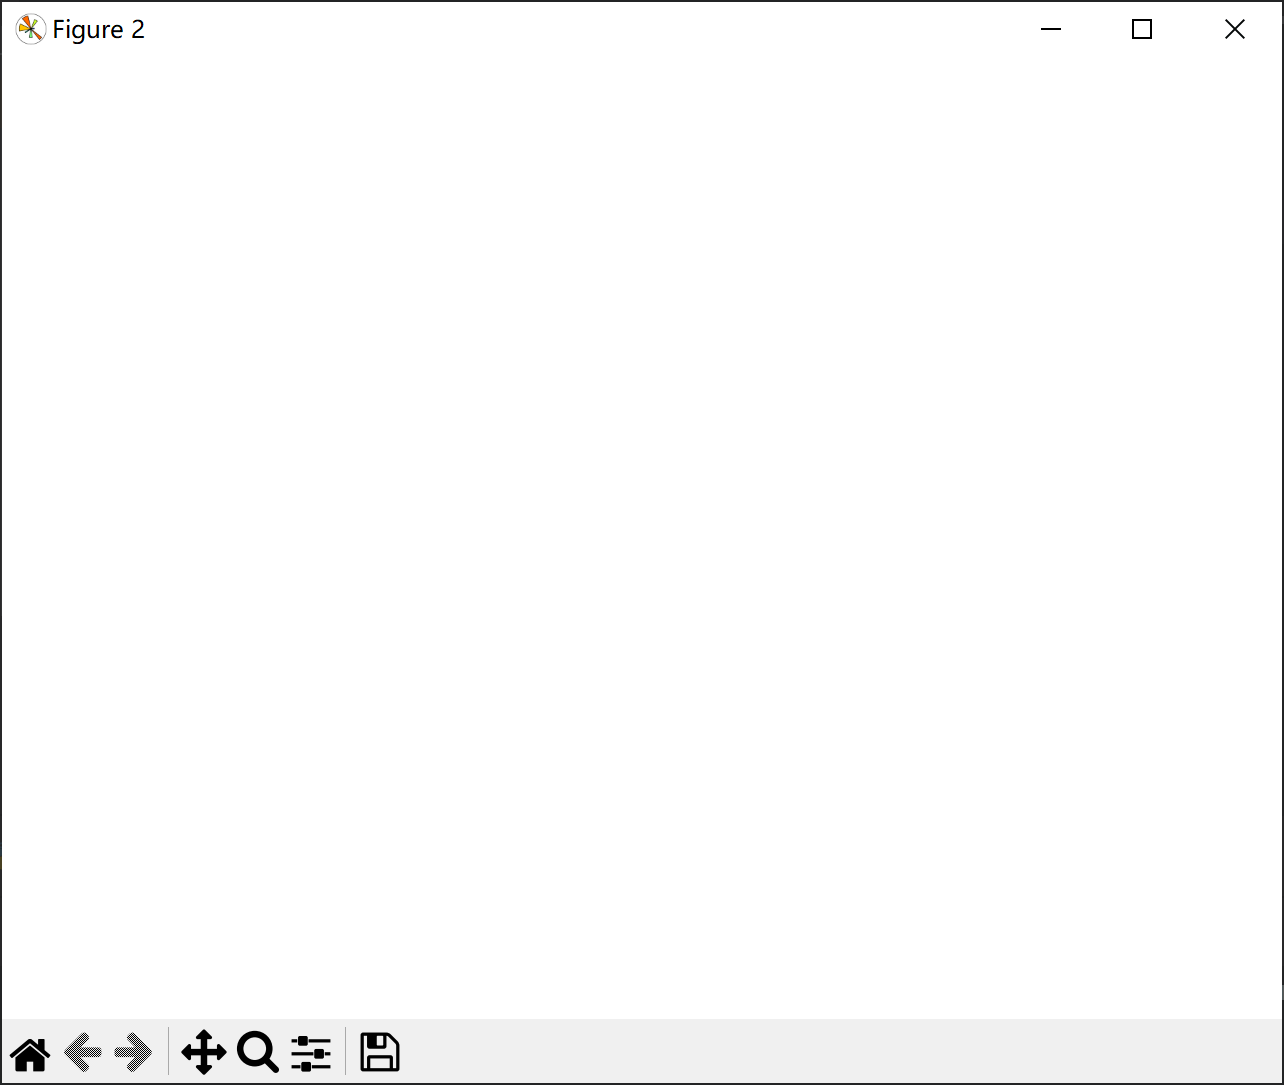
\includegraphics[width=0.5\linewidth]{图形对象样例.png}
    \caption{2.1.1}
    \label{fig:enter-label}
\end{figure}
而子图则是生成的坐标轴和绘制出的精美的图形,如下图:
\begin{figure}[H]
    \centering
    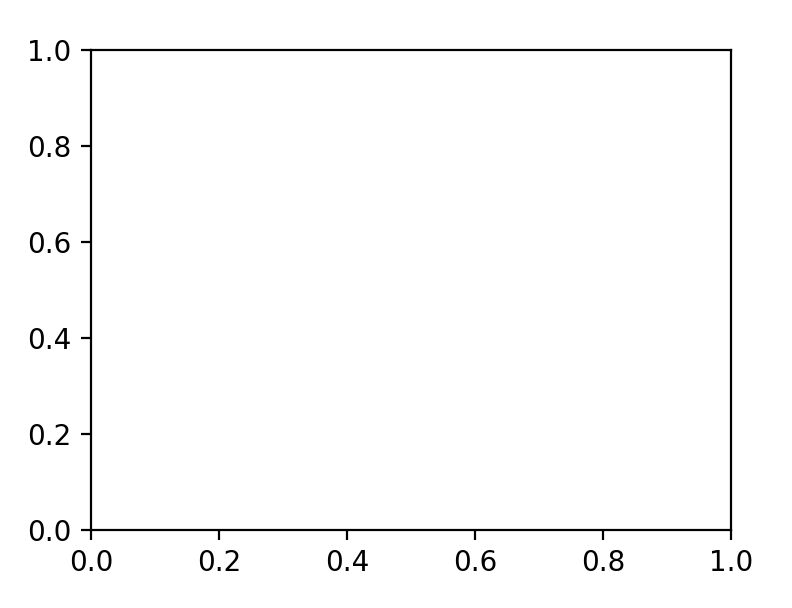
\includegraphics[width=0.5\linewidth]{子图样例.png}
    \caption{2.1.2}
    \label{fig:enter-label}
\end{figure}
其实,我们也可以把子图理解为坐标轴,而绘图的过程是对坐标轴实施的操作。

明晰了这两个概念后,我们就可以把Matplotlib绘图的过程视为创建图形对象——创建子图——对子图进行操作的过程。

如何创建图形对象和坐标轴呢?有以下方法:

1. fig = plt.figure()

这是通过plt.figure()创建了一个图形对象,并赋值给fig,从而后面我们可以通过“fig”来对这个图形对象进行操作。

2. 如果后面在绘图时使用plt.plot()命令,那么我们是不需要创建图形对象的,因为当你调用 plt.plot 时,如果当前没有活跃的坐标轴(连一个图形对象都没有,当然不会有活跃的坐标轴),matplotlib 会自动创建一个新的图形和一个默认的坐标轴。

上述两种方法分别对应了对Axes和pyplot这两个Matplotlib库中用于绘图的主要接口的使用。如果使用Axes绘图,我们需要提前创建一个图像对象,而使用pyplot则不需要,这使得其使用更加简便,易于上手。除此之外,Axes和pyplot的区别还有:

\noindent\textbf{Pyplot:}

1. pyplot允许链式调用,即在一行代码中连续调用多个方法,例如:
% \[plt.plot(x, y).title('My Plot').xlabel('X-axis').ylabel('Y-axis').show()
% \]
\begin{figure}[H]
    \centering
    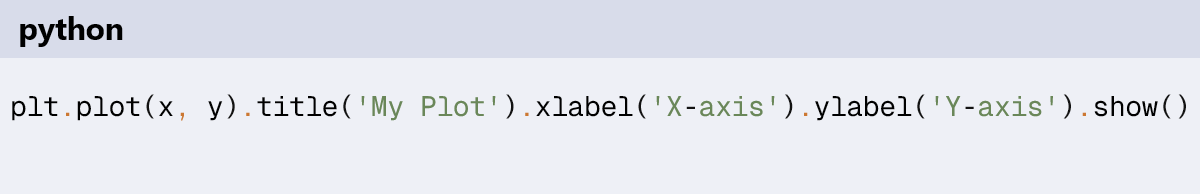
\includegraphics[width=1\linewidth]{1.png}
    \caption{2.2.1}
    \label{fig:enter-label}
\end{figure}
2. 还有就是我们刚才说的,使用pyplot不需要提前创建图形对象,这是因为pyplot具有自动管理功能,它能够自动为你管理图形和轴对象,你不需要显式地创建它们。当你调用   plot 、scatter等方法时,pyplot会在后台为你创建或更新当前的图形和轴。

\noindent\textbf{Axes:}

1. 更多的控制:  Axes   提供了更多的方法来自定义和控制图表的各个方面,比如设置轴的刻度、添加注解、调整轴的显示范围等。

2. 面向对象:使用   Axes   时,你可以直接与图表的轴对象交互,这使得你可以更精确地控制图表的布局和外观。

3. 多个子图:当你需要在一个图形窗口中创建多个子图时,  Axes   提供了更好的支持。你可以创建多个   Axes   实例,并将它们放置在不同的位置上。

4. 高级功能:  Axes   支持一些高级功能,比如共享轴、对数轴、极坐标轴等,这些在   pyplot   中可能不那么直观。

接下来我会分别介绍pyplot和Axes的一些基本用法。

\section{Pyplot的基本用法}
在matplotlib绘图程序的开头通常有一个导入:import matplotlib.pyplot as plt. 这里所做的就是导入了matplotlib库里的pyplot类,并将其简称为plt。后面程序中出现以plt.为前缀的命令就是在调用pyplot的方法。

\subsection{Pyplot绘图的基本方法}
% \noindent\textbf{\large 线图}
\subsubsection{线图}
线图,顾名思义,就是将所有离散的点连成线的图像。绘制线图有两种基本操作:

方法1: 指定x的取点范围和密度,然后指定x——>y的映射关系(写出函数表达式),最后plt.plot(x,y)。

方法2: 直接指定所有图像中确定经过的点的x,y坐标,放在plt.plot指令中即可实现。

注意plot作为线图绘制的方法函数,其本质是将所有离散的点以直线相连,这一点在运用方法2的时候尤为明显,而方法1由于可以指定取点密度,只要我们将点密度设得足够大,最后呈现的效果就是平滑的曲线(方法2你总不可能手动输入100个点的坐标吧)。

下面我们以一个简单的函数\(y=x^2\)为例,展示这两个方法如何运用。

\textbf{\large 方法1}:
\begin{figure}[H]
    \centering
    \begin{subfigure}[b]{0.45\textwidth}
        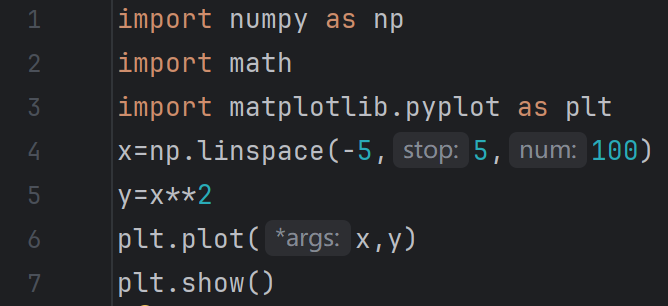
\includegraphics[width=1.2\textwidth,height=0.6\textwidth]{线图2.png}
        \caption{使用np.linspace}
        \label{fig:enter-label-1}
    % \centering
    
    \end{subfigure}
    \hfill        
    \begin{subfigure}[b]{0.45\textwidth}
        % \centering
        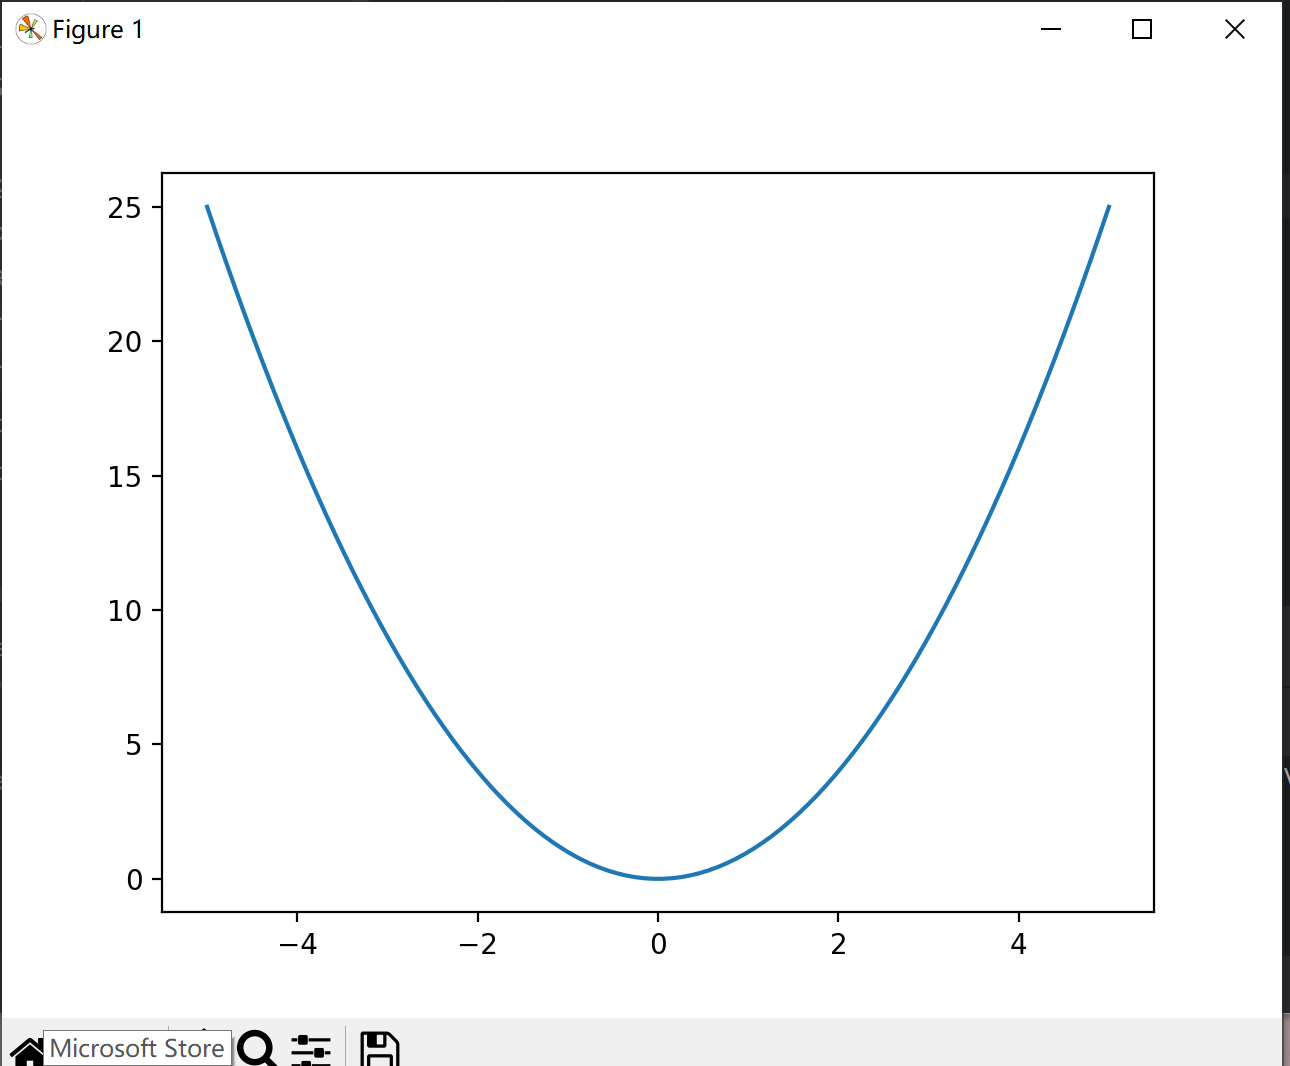
\includegraphics[width=0.8\textwidth]{线图 pic2.png}
        \caption{Gragh of \(y=x^2\)}
        \label{fig:enter-label-2}
    \end{subfigure}
\end{figure}

np.linspace(a,b,n)函数能够返回一个numpy数组,其中a和b分别是这个数组的起始点与终止点,n则是在这个区间内的取点数量,通常取点数减一与区间长度的商如果是有限小数的话,它的取点是等分的。(但我们大量取点拟合曲线的时候,这件事并不重要)

如果我们少取一些点,比如只取10个点,就可以明显看出plot实质上是以直线拟合曲线:

\begin{figure}[H]
    \centering
    \begin{subfigure}[b]{0.45\textwidth}
        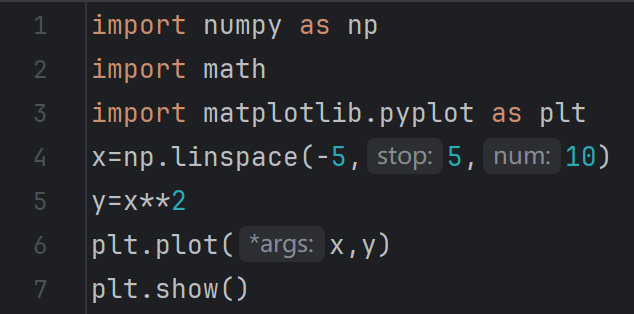
\includegraphics[width=1.2\textwidth,height=0.6\textwidth]{线图1.png} % 确保图片宽度不超过页面宽度
        \caption{使用np.linspace,但是只有10个点}
        \label{fig:line-graph2}
    \end{subfigure}
    \hfill
    \begin{subfigure}[b]{0.45\textwidth}
        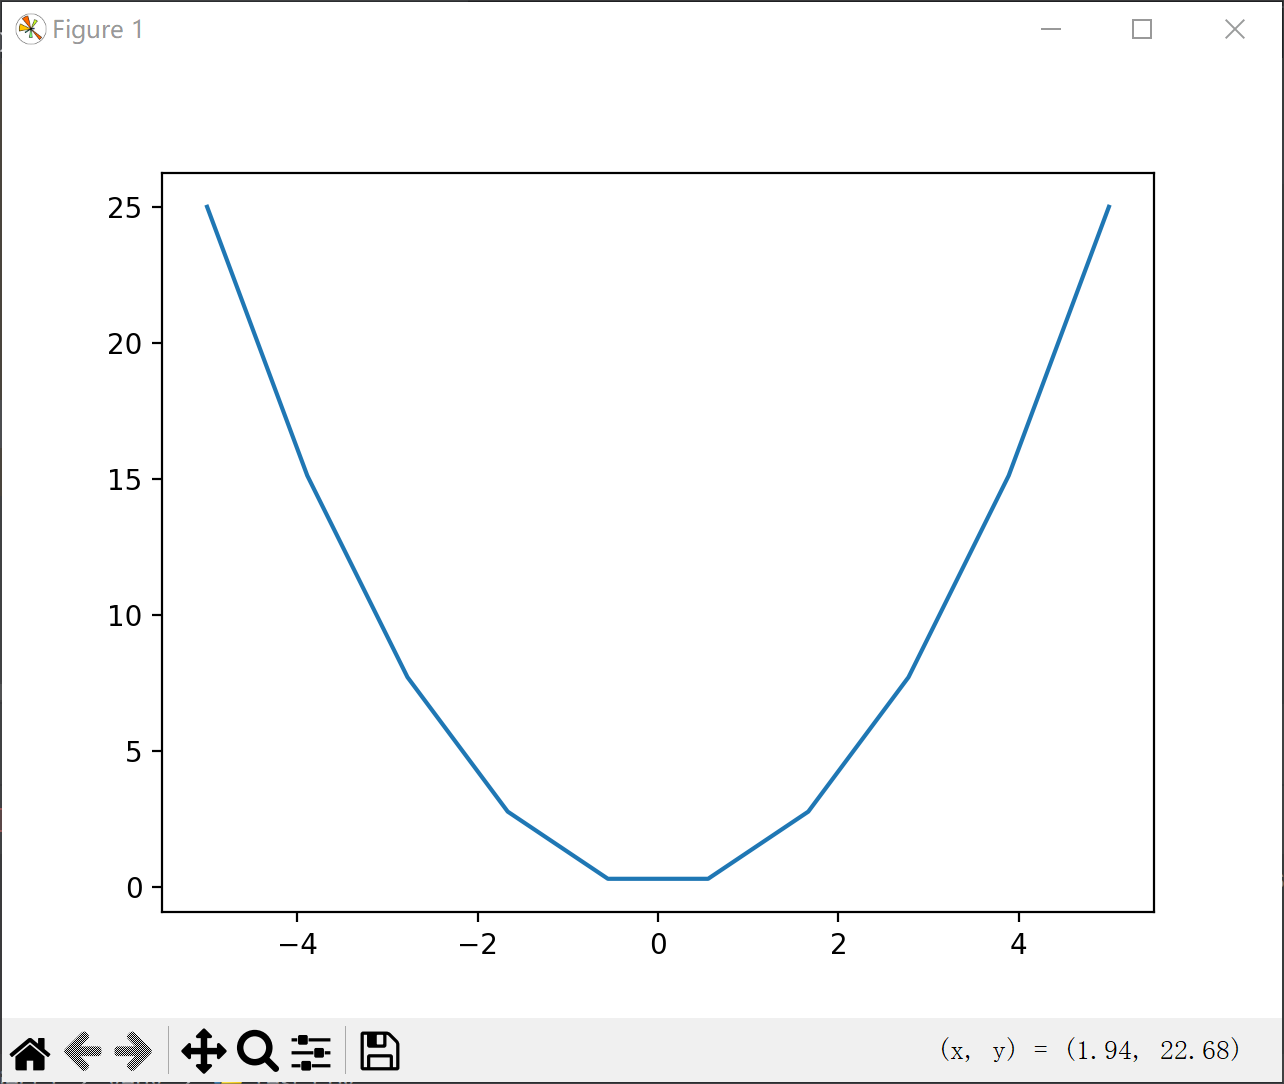
\includegraphics[width=\textwidth]{线图 pic1.png} % 确保图片宽度不超过页面宽度
        \caption{Graph}
        \label{fig:line-graph2-pic2}
    \end{subfigure}
\end{figure}

plot只能实现以直线连接各点,如果我们想要让各点以平滑曲线相连,而不采用暴力增加点数的方法呢?方法也是有的,那就是用多项式拟合,其中涉及到对scipy.fsolve等函数的使用,我们放在“详述"~\ref{如何利用Python解方程}中细说。

在这里要注意区分numpy数组和一般的Python列表,它们有许多区别和联系,对此的完整介绍我放在“详述”~\ref{numpy数组与列表,元组}部分,这里只说一点,就是numpy数组支持向量化计算,而列表不支持。向量化计算就是在背景知识——数学运算中提到的对一个数组进行单个数值形式的运算,输出一个由所有元素计算结果组成的新数组。简单来说,在Python中,array1+array2是合法的,但是list1+list2是不合法的,同样的规则适用于其它单个数值基本运算。如图3.1.5所示,这段代码会报错。因为我们最后是通过当数值的运算构建由x到y的映射关系的,所以如果x是一个列表(或者元组),我们就无法对它(整个x)直接进行运算操作,解决办法有两个,一是使用for循环把元素一一提取出来映射到y,如图3.1.6所示,plot函数似乎既可以接受array也可以接受list作为输入。
\begin{figure}[H]
    \centering
    \begin{subfigure}[b]{0.45\textwidth}
        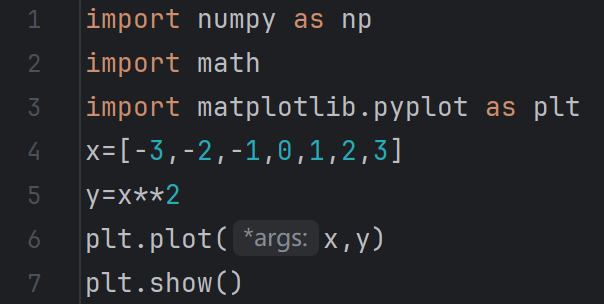
\includegraphics[width=1.2\textwidth,height=0.6\textwidth]{线图 错误示范1.png}
        \caption{3.1.5错误示范}
        \label{fig:enter-label-1}
    % \centering
    
    \end{subfigure}
    \hfill        
    \begin{subfigure}[b]{0.45\textwidth}
        % \centering
        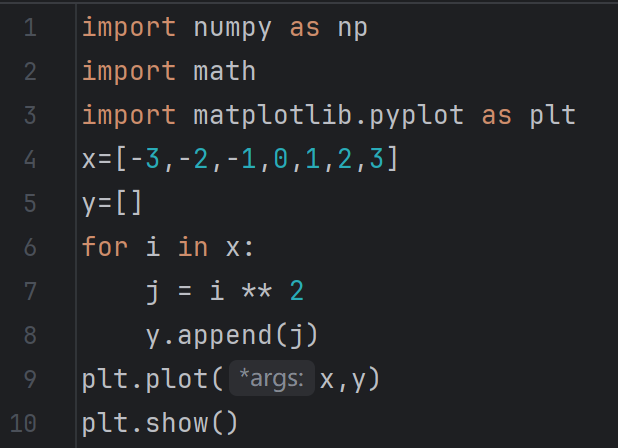
\includegraphics[width=\textwidth]{线图 正确示范1.png}
        \caption{3.1.6正确示范}
        \label{fig:enter-label-2}
    \end{subfigure}
\end{figure}
另一个办法是将列表转换为numpy数组形式,元组和列表均可以由以下方式转换:x=np.array([ ])或x=np.array(( ))。示例如下3.1.7:
\begin{figure}[H]
    \centering
    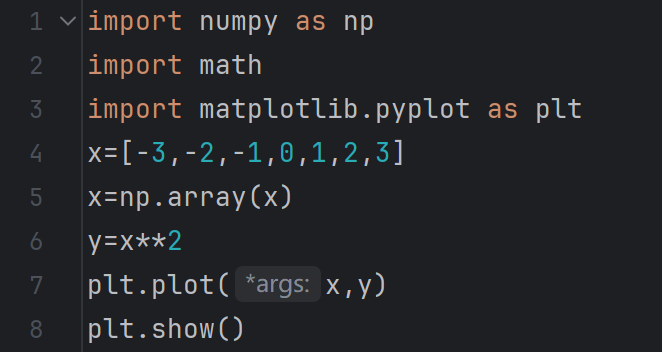
\includegraphics[width=0.6\linewidth]{转array示范.png}
    \caption{3.1.7}
    \label{fig:enter-label}
\end{figure}

\textbf{\large 方法2}

我们直接取几个整点,列出它们的x,y坐标,x,y各列成一个数组的形式,然后直接丢给plot函数,plot就可以把所以点以直线相连形成线图。如3.1.8和3.1.9所示:

\begin{figure}[H]
    \centering
    \begin{subfigure}[b]{0.45\textwidth}
        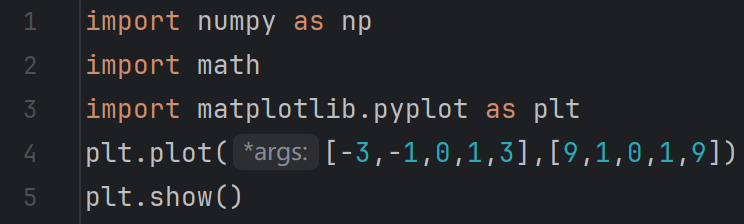
\includegraphics[width=1.2\textwidth,height=0.45\textwidth]{线图方法2 2.png}
        \caption{3.1.8}
        \label{fig:enter-label-1}
    % \centering    
    \end{subfigure}
    \hfill        
    \begin{subfigure}[b]{0.45\textwidth}
        % \centering
        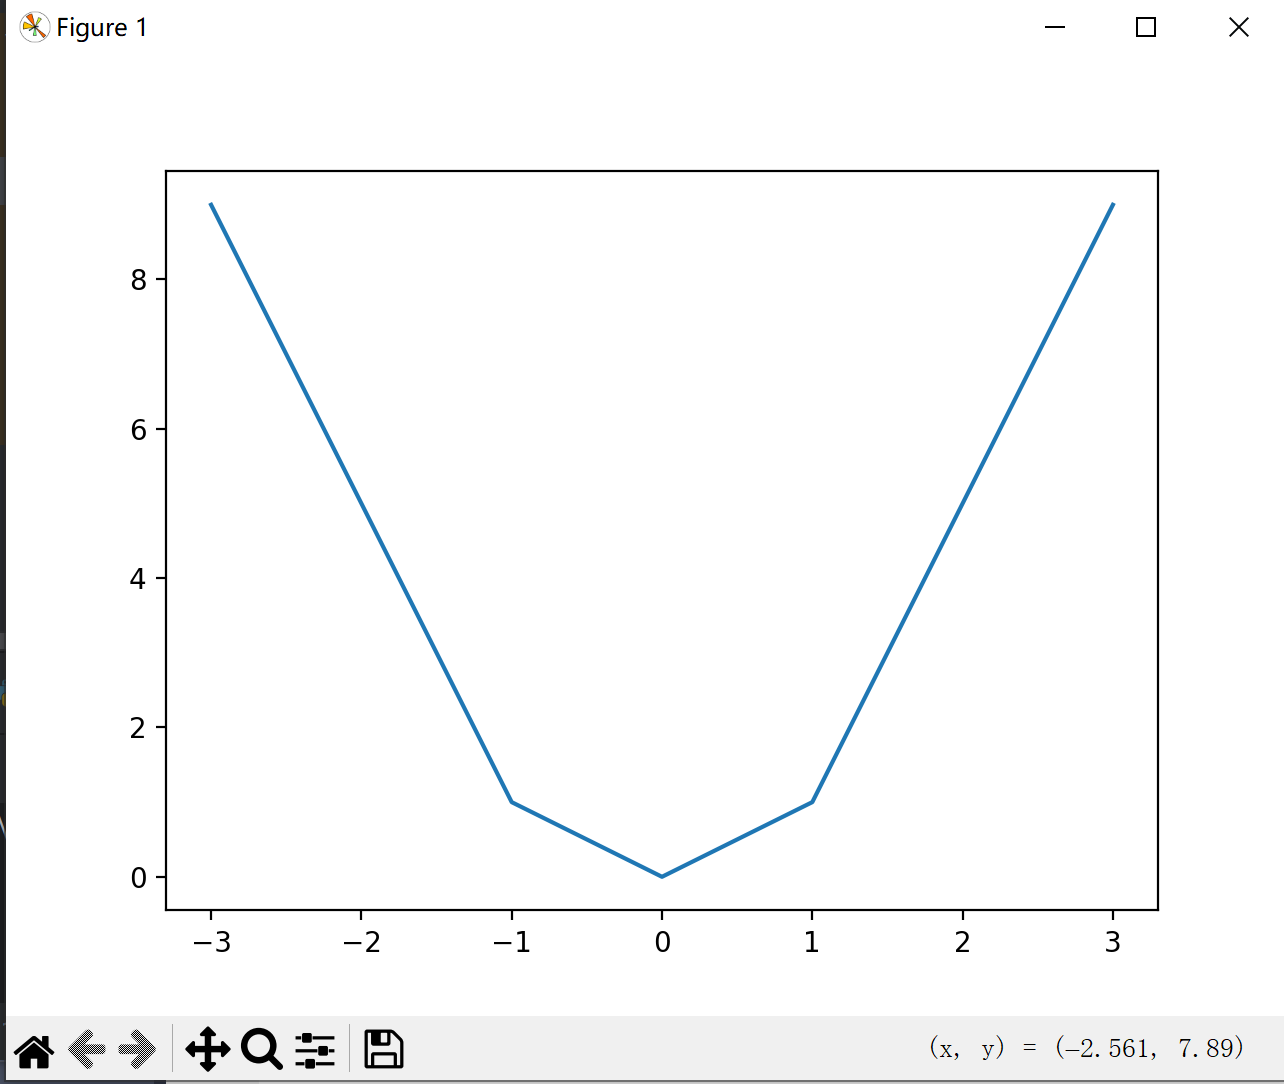
\includegraphics[width=\textwidth]{线图方法2 Pic.png}
        \caption{3.1.9}
        \label{fig:enter-label-2}
    \end{subfigure}
\end{figure}


除了接受点数据绘制折线图外,plot函数还支持对线图的许多属性进行设定,包括颜色,粗细,实虚样式以及图例等等。
\[plt.plot(x,\,y,\,color='\,',\,linewidth=\quad,\,linestyle='\,',\,label='\,')\]
举个例子,我如果希望把函数\(y=x^2\)的图像设置为红色,线宽为1.5,虚线,代码与效果如图所示:

\begin{figure}[H]
    \centering
    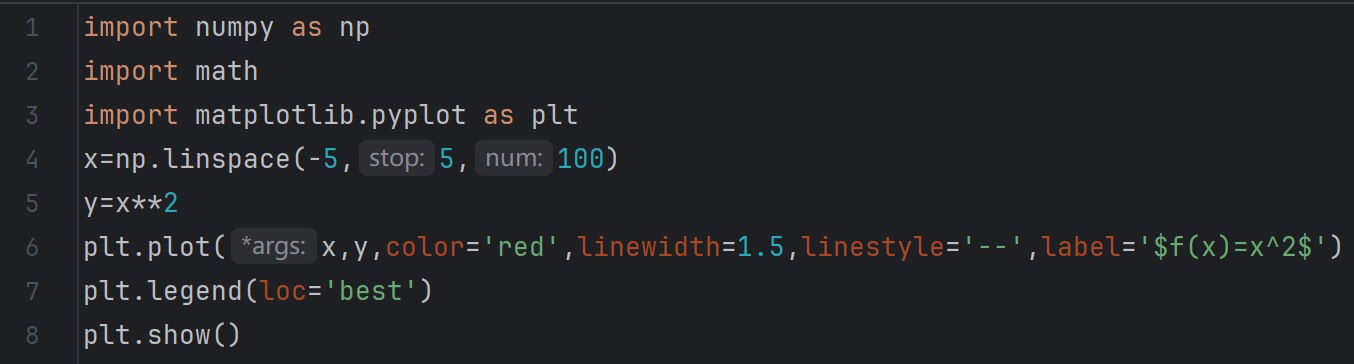
\includegraphics[width=1\linewidth]{plot函数的其他设定 program.png}
    \caption{3.1.10}
    \label{fig:enter-label}
\end{figure}
\begin{figure}[H]
    \centering
    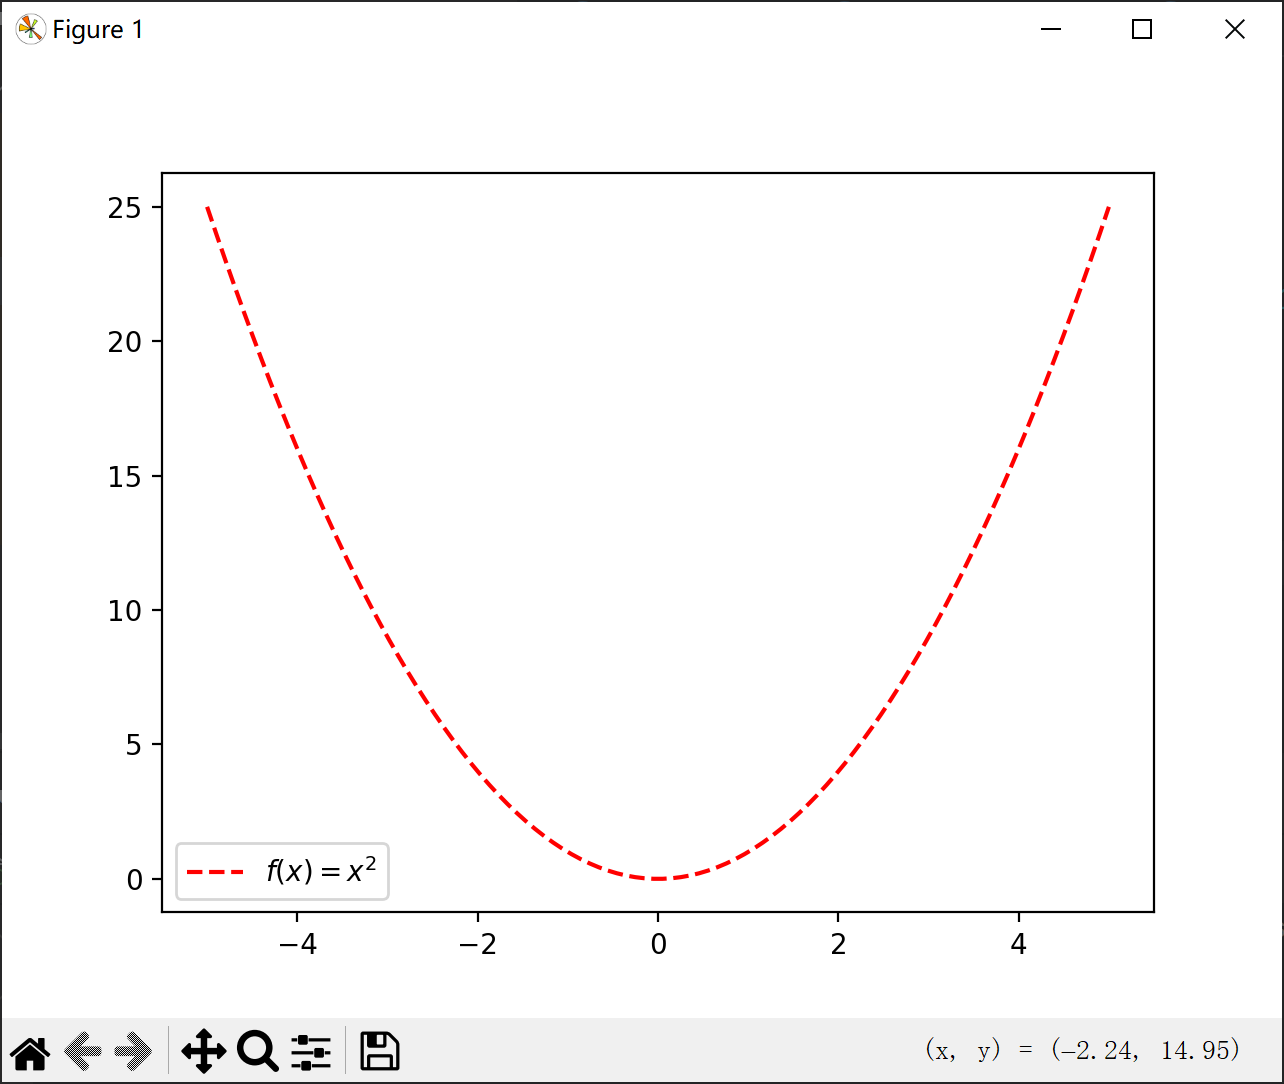
\includegraphics[width=0.75\linewidth]{plot函数的其他设定 picture.png}
    \caption{3.1.11}
    \label{fig:enter-label}
\end{figure}

\noindent 对于linestyle,尽管不同线形有相应的单词代称,比如实线是"solid",但是多数时候我们更习惯用标点来指代线形,如下表所示:
\begin{table}[H]
\centering
\begin{tabularx}{0.8\textwidth}{|c|>{\centering\arraybackslash}X|c|>{\centering\arraybackslash}X|X|}
实线         & 'solid'   & '-'  \\
虚线         & 'dashed'  & '--' \\
点线         & 'dotted'  & ':'  \\
点划线        & 'dashdot' & '-.' \\
无线条(仅显示标记) & 'None'    & ' ' 
\end{tabularx}
\end{table}
\noindent 对于图例,图例上显示的名字是在plot中的label设定的那个名字,然后调用图例函数plt.legend()即可生成图例,在图例函数中,可以通过loc=' '来指定图例在图中的摆放位置,比如loc='best'指将其摆放到系统认为最合适的位置,即图像最稀疏(对图像影响最小)的地方。legend还可以进行其它的设定,放在”详述“~\ref{图例的高级设置}里讲。

% \noindent\textbf{\large }
\subsubsection{点图}
点图就是离散的点组成的图像,使用scatter函数,把在线图举的例子中的plot函数换成scatter函数,就可以生成一张\(y=x^2\)点图。
\begin{figure}[H]
    \centering
    \begin{subfigure}[b]{0.45\textwidth}
        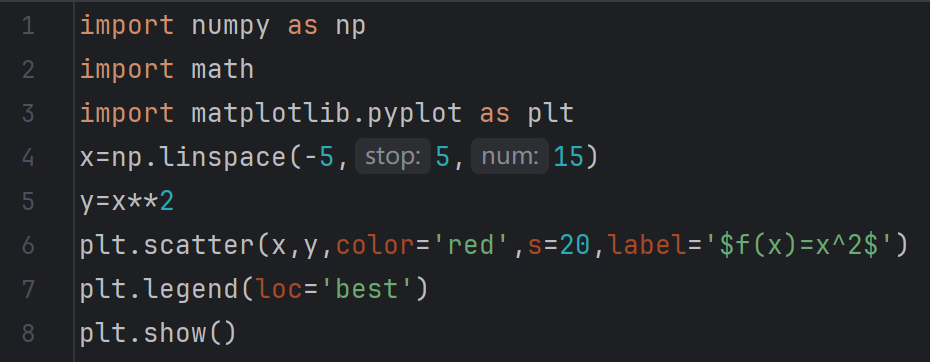
\includegraphics[width=1.3\textwidth,height=0.6\textwidth]{点图program1.png}
        \caption{3.2.1}
        \label{fig:enter-label-1}
    % \centering    
    \end{subfigure}
    \hfill        
    \begin{subfigure}[b]{0.4\textwidth}
        % \centering
        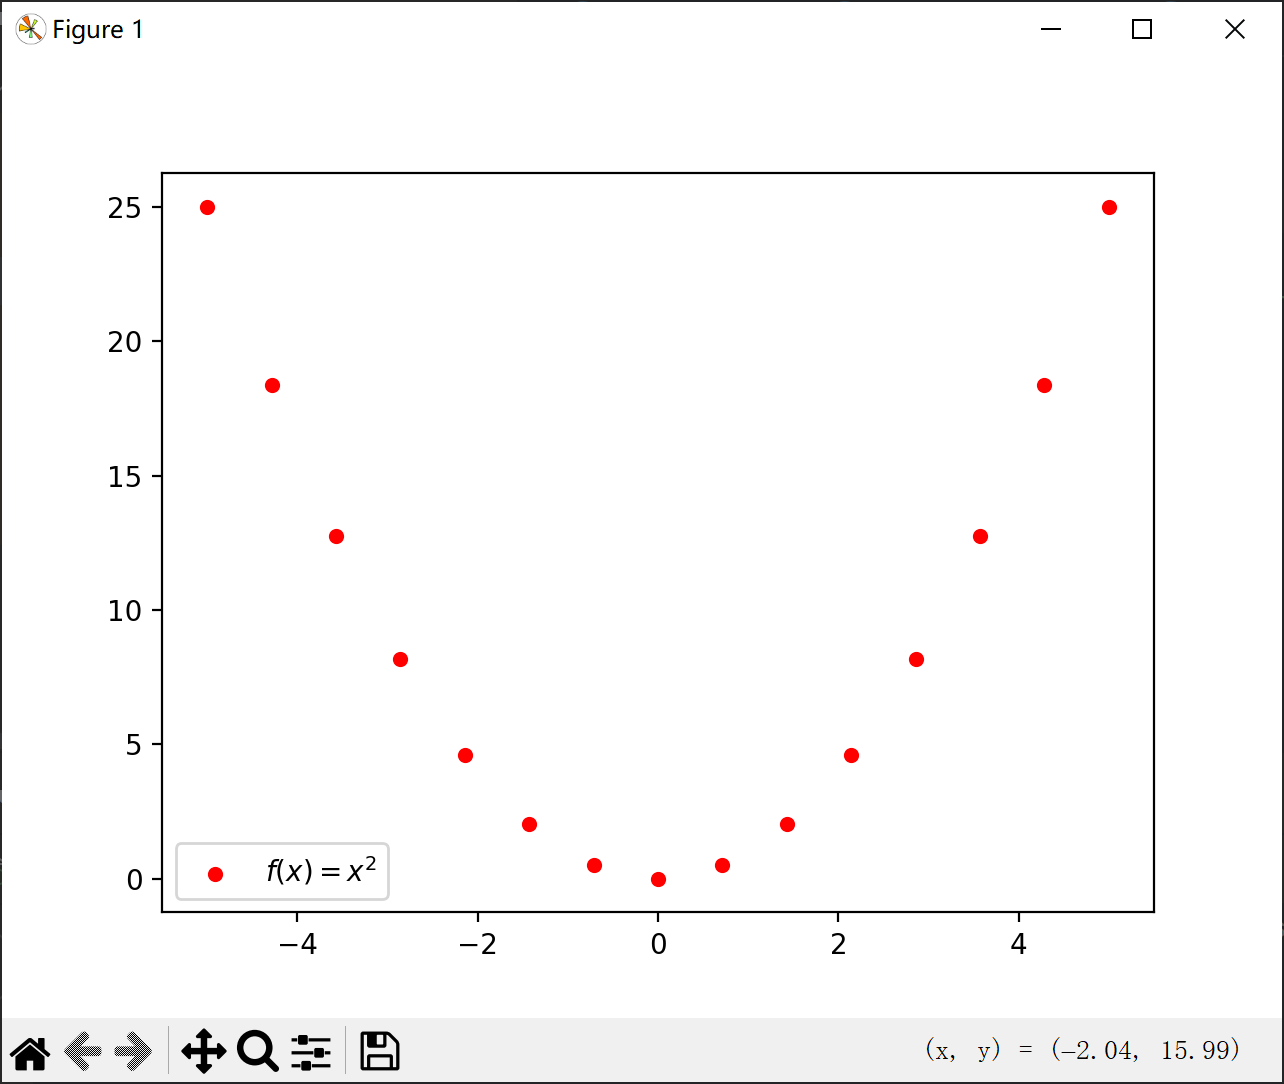
\includegraphics[width=\textwidth]{点图Pic1.png}
        \caption{3.2.2}
        \label{fig:enter-label-2}
    \end{subfigure}
\end{figure}

与plot相同的是,x,y处都可以接受数组,列表,都可以设置颜色。不同的是,scatter的x,y可以仅接受一个点坐标,而plot遇到这种情形则会报错。
还有一个与线图属性的设置不同的地方,是点图没有所谓的线宽参数linewidth,取而代之的是点宽参数s,上图代码中的\(s=20\)就是将点宽设成了20。(特别注意一点,这里的s不是size的简写!!!如果在这里写size反而会报错,关于简写使用的问题在详述中会详细讨论~\ref{简写问题}),s是一个数值时,这个数值指定了所有点的点宽;此外s还可以是一个数组或列表或元组,其中每个元素指定对应的点的大小,要注意的是它的元素数必须与x,y的元素数一样,否则会报错。


\begin{figure}[H]
    \centering
    \begin{subfigure}[b]{0.5\textwidth}
        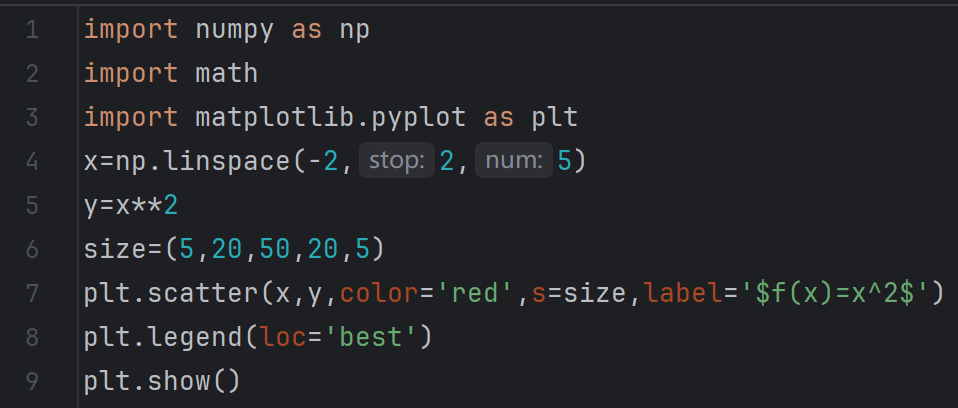
\includegraphics[width=\textwidth]{点图program2.png} % 确保图片宽度不超过页面宽度
        \caption{3.2.3}
        \label{fig:line-graph2}
    \end{subfigure}
    \hfill
    \begin{subfigure}[b]{0.45\textwidth}
        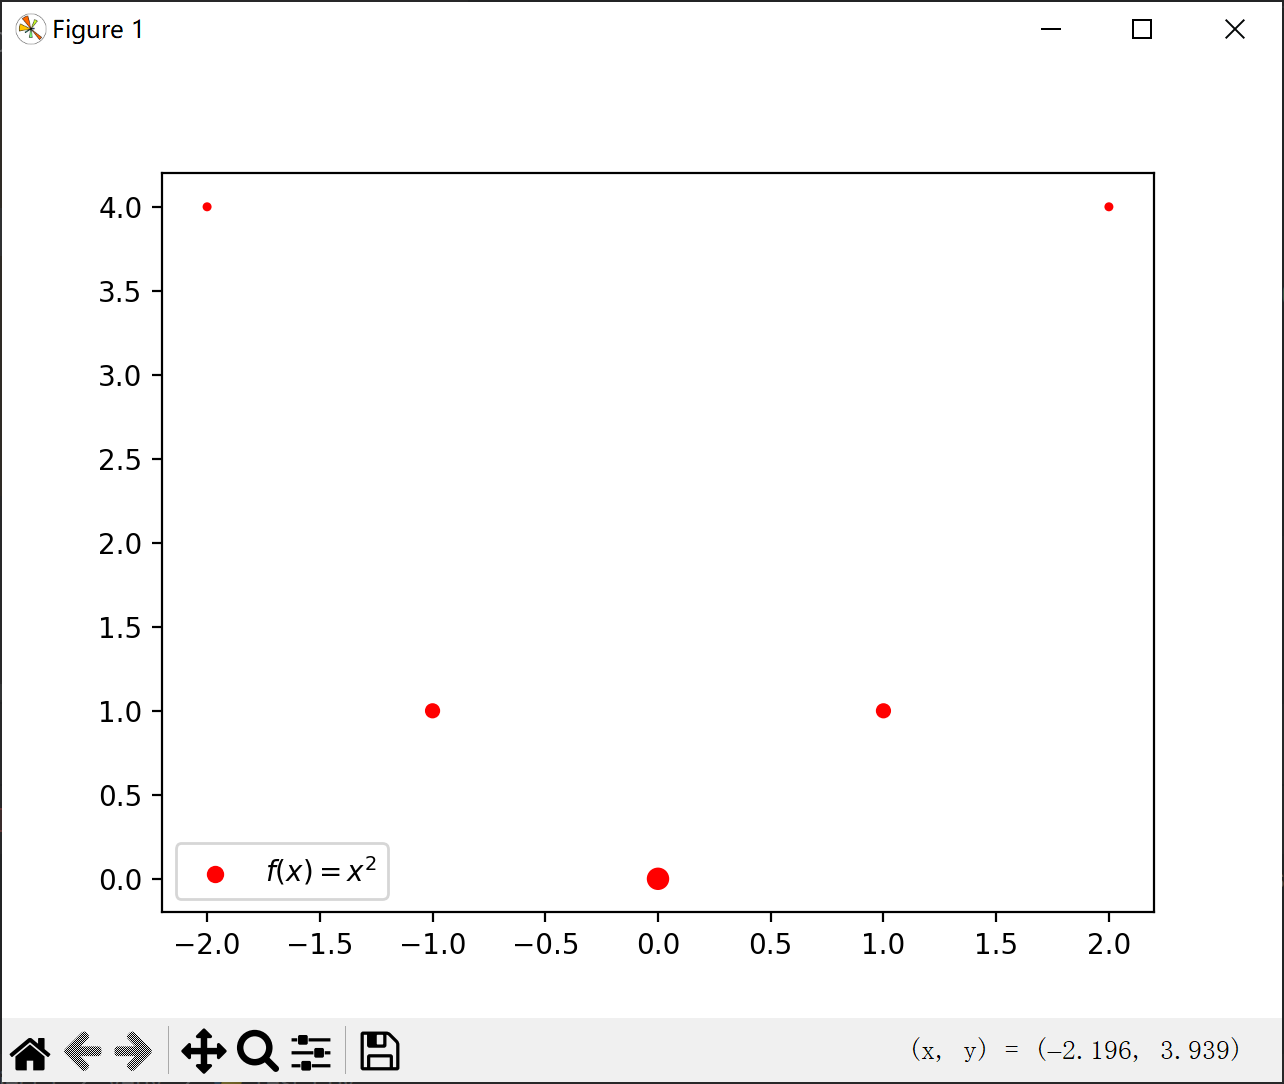
\includegraphics[width=\textwidth]{点图Pic2.png} % 确保图片宽度不超过页面宽度
        \caption{3.2.4}
        \label{fig:line-graph2-pic2}
    \end{subfigure}
\end{figure}
还有一个重要的不同,scatter函数支持颜色,宽度,透明度作为数组传递给相应的参数,但是plot函数不支持,像下面这么写,在scatter里面没问题,但是在plot里面就会报错。
\begin{figure}[H]
    \centering
    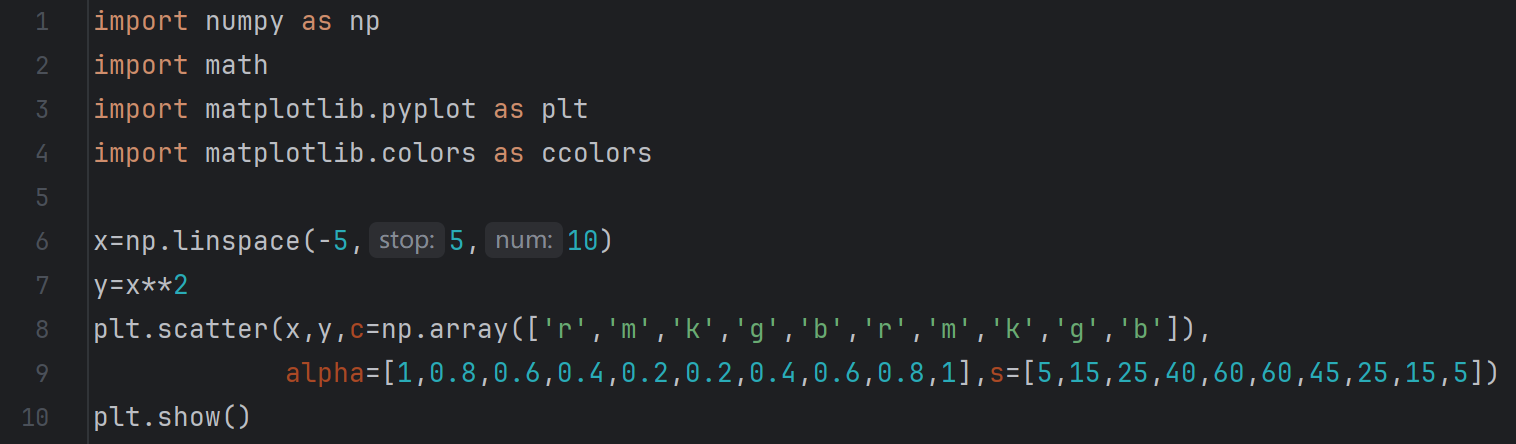
\includegraphics[width=1\linewidth]{点图program3.png}
    \caption{3.2.5}
    \label{fig:enter-label}
\end{figure}
\begin{figure}[H]
    \centering
    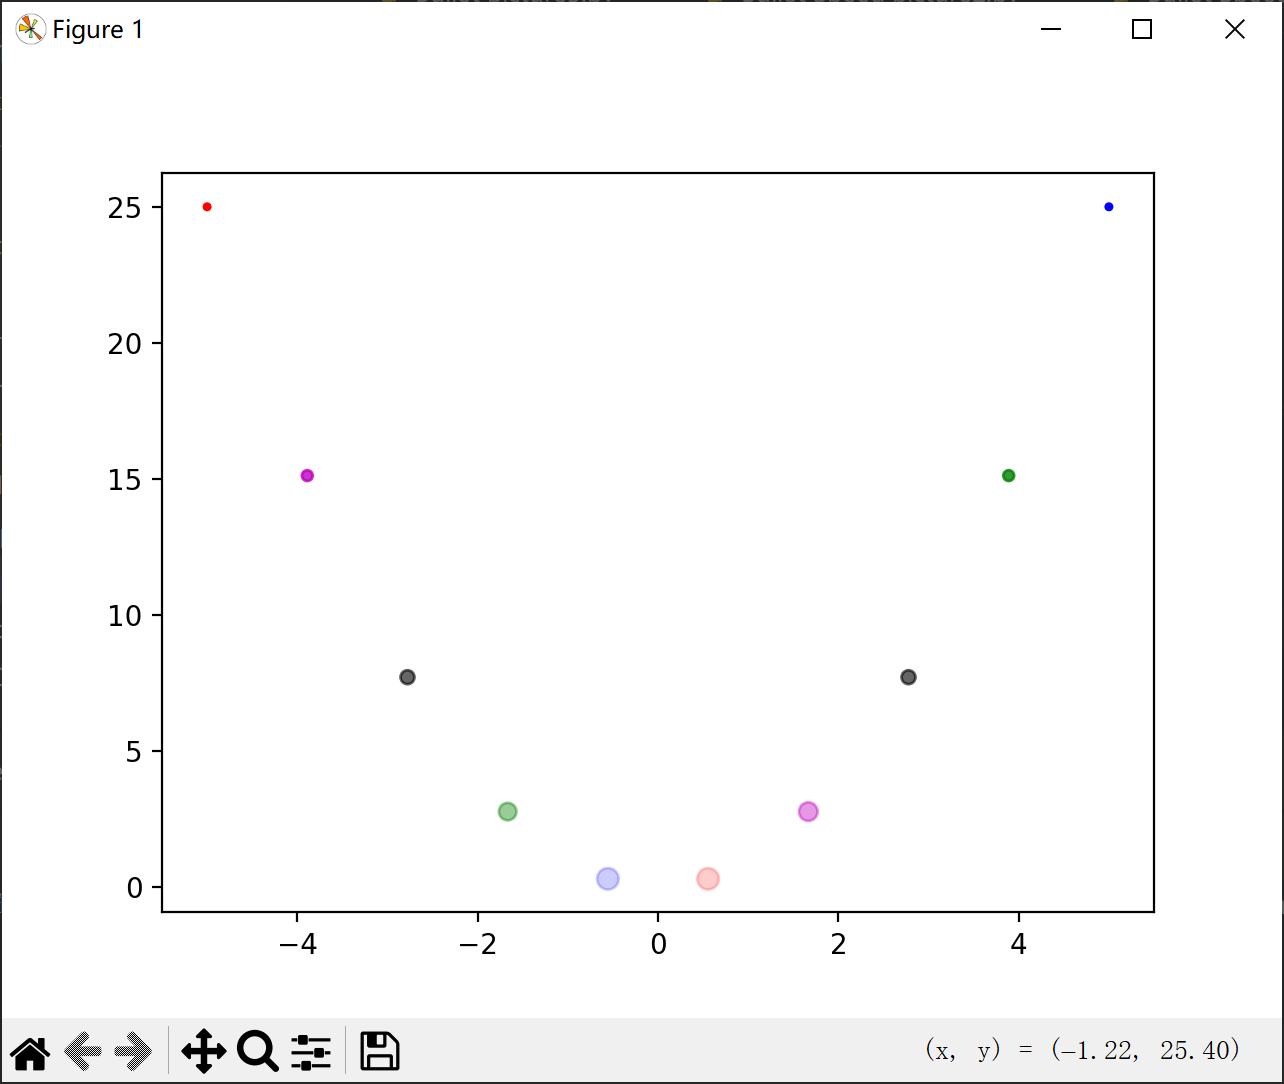
\includegraphics[width=0.75\linewidth]{点图Pic3.png}
    \caption{3.2.6}
    \label{fig:enter-label}
\end{figure}
(还要注意一件事,当我们向颜色传递数组类参数时,必须使用简写形式” c=' ' “,传递单个参数时则不需要,不要问我为什么。总而言之,color参数用于设置统一的颜色,而c参数既用于根据数值数组来映射颜色,也用于在设置统一的颜色时,作为color的简写。)

总之,scatter的常用设置包括颜色,点宽,图例,其他高级的设置我们放到”详述“~\ref{scatter函数的高级设置}。

\subsubsection{条形图}
条形图的核心由两要素组成,一是类别(x轴),二是数值(y轴),每个类别对应一个数值。因此绘制一张基本的条形图需要两个列表,分别存储类别和数值,然后类似plot函数的做法,将这两个列表传递给条形图函数bar()。以下是一个示例:
\begin{figure}[H]
    \centering
    \begin{subfigure}[b]{0.5\textwidth}
        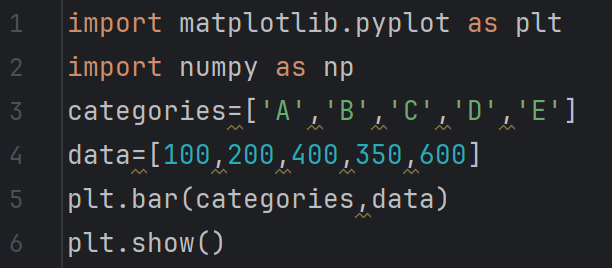
\includegraphics[width=\textwidth]{条形图 program1.png} % 确保图片宽度不超过页面宽度
        \caption{3.1.2.1}
        \label{fig:line-graph2}
    \end{subfigure}
    \hfill
    \begin{subfigure}[b]{0.45\textwidth}
        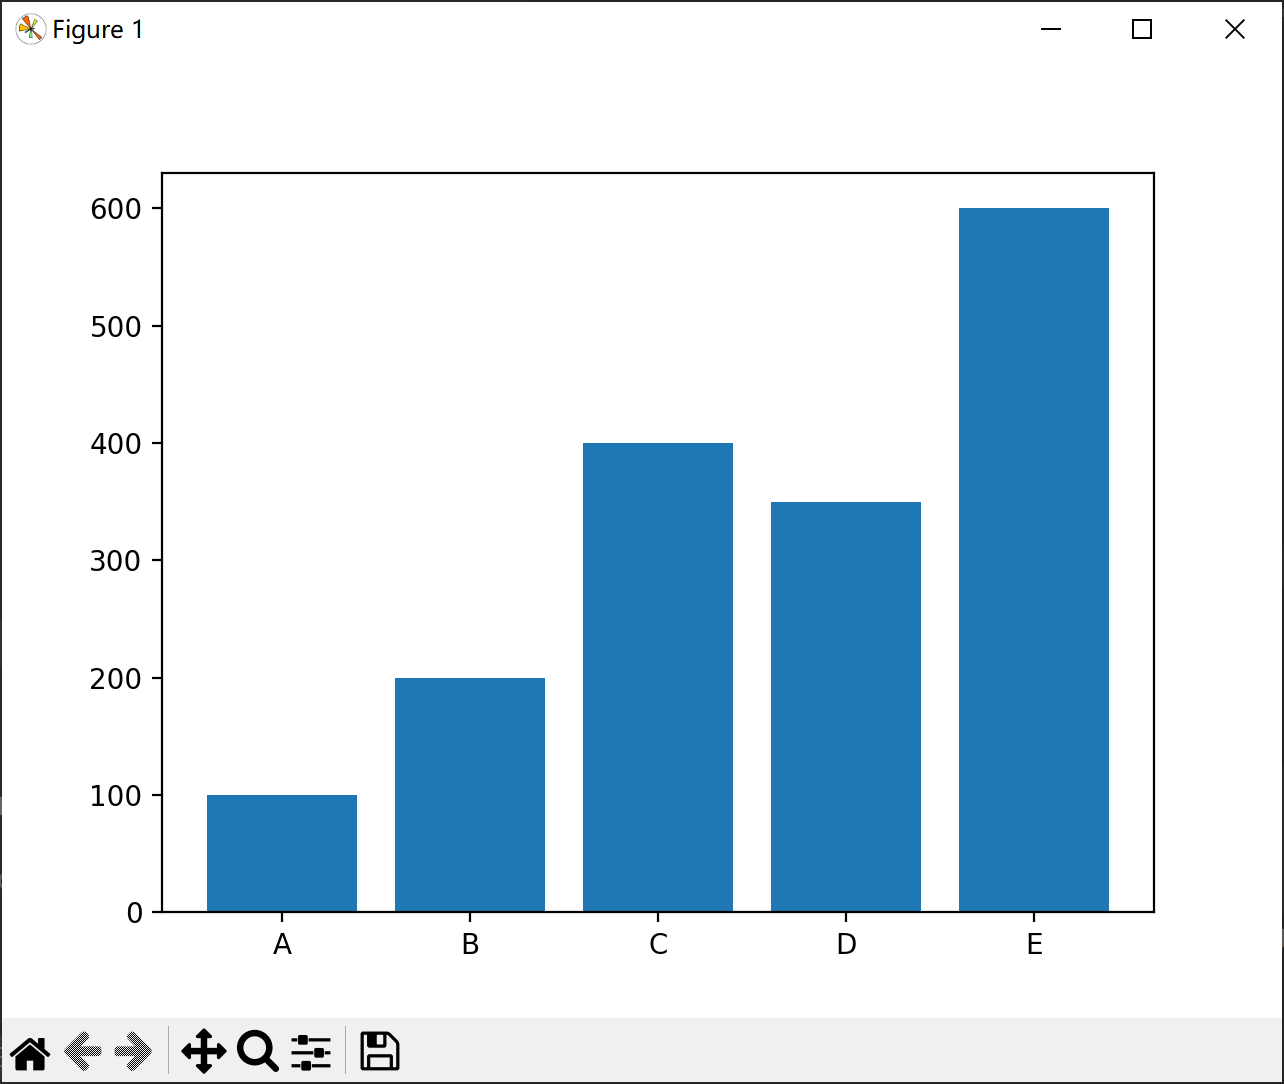
\includegraphics[width=\textwidth]{条形图 Pic1.png} % 确保图片宽度不超过页面宽度
        \caption{3.1.2.2}
        \label{fig:line-graph2-pic2}
    \end{subfigure}
\end{figure}
\noindent 注意一件事,x轴上的类别其实是有绝对宽度的,每两个类别的间距比如上图的A-B的间距是1,而每个类别的条宽默认是0.8,这个条宽是可以调整的,方法是width= ,数值应该在(0,1],width=1时所有条是紧挨的。

除了条宽,其它设置包括颜色、边缘颜色、透明度、图例、对齐方式、数值标签。颜色是color,边缘颜色是edgecolor,透明度是alpha,图例是label加legend函数,这些都跟plot和scatter一样,不再赘述。下面重点介绍对齐方式和数值标签。

\noindent\textbf{对齐方式}

对齐方式指的是每个条形与x轴上的类别的相对位置,方法是align= ,align='center'时是图3.1.2.2所示的中心对齐,因此这其实是默认的状态,我们还可以令align='edge',此时是边缘对齐,如图3.1.2.3所示:
\begin{figure}[H]
    \centering
    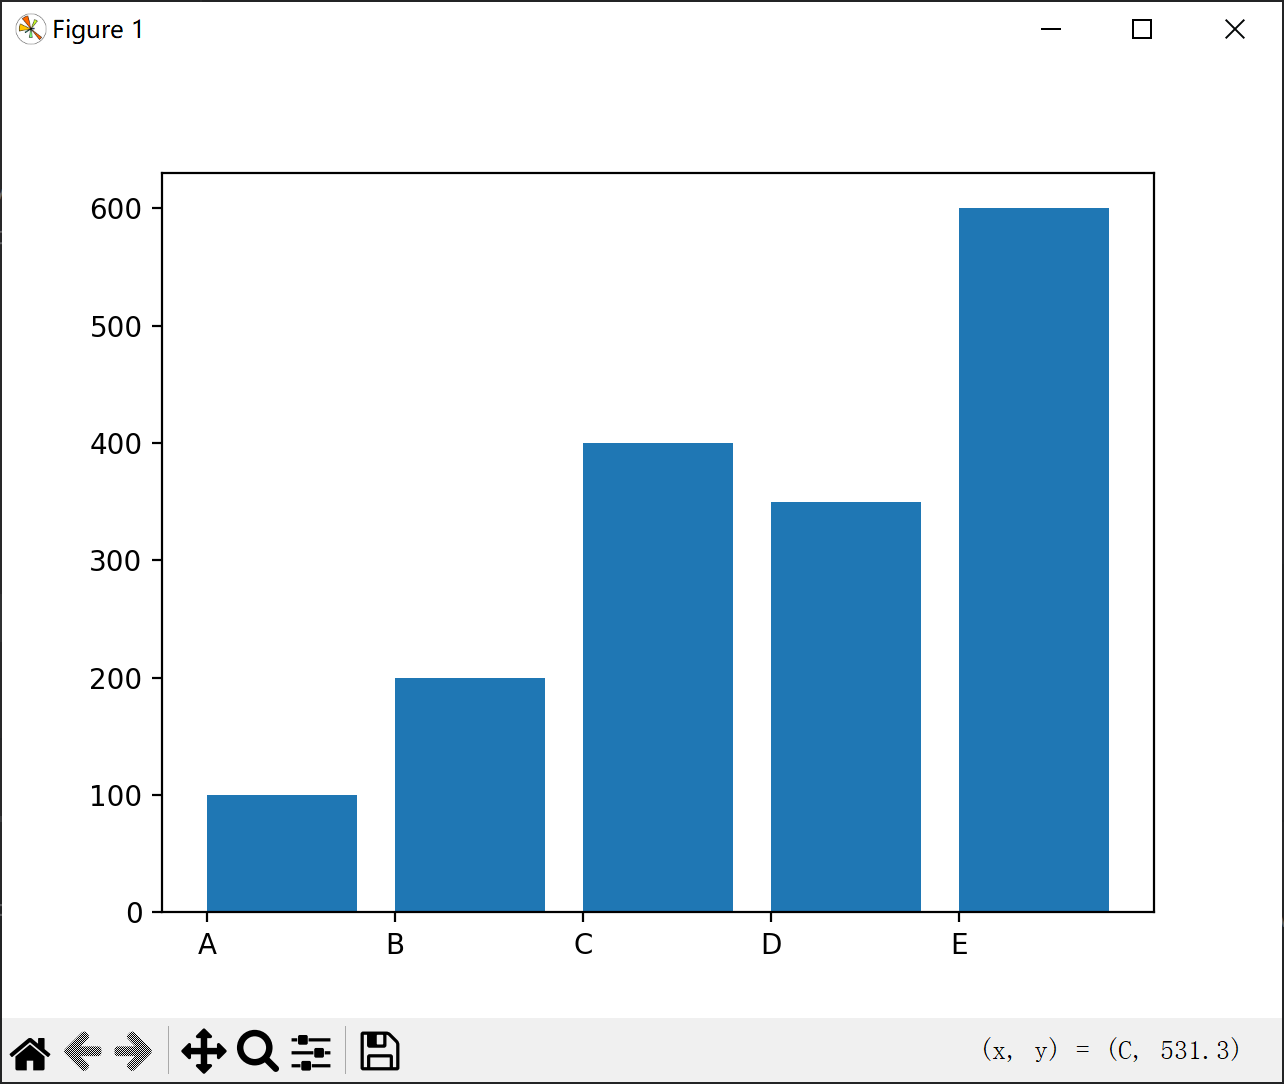
\includegraphics[width=0.4\linewidth]{条形图 Pic2.png}
    \caption{3.1.2.3}
    \label{fig:enter-label}
\end{figure}
(按理来说应该可以用left和right指定左右对齐的,但是不知道为什么在Pycharm里好像不行)

\noindent\textbf{数值标签添加}

有时我们需要把每一类的数值标在条形上方,这时我们需要enumerate,它是一个很有用的Python内置函数,能同时返回可迭代对象中元素的索引值和数据值。其基本语法为enumerate(可迭代对象, 起始索引),其中起始索引不指定的话默认是0,此时enumerate会从头开始遍历整个对象。enumerate 会返回一个枚举对象,这个对象可以被用来在循环中同时获取索引和值。这个对象是一个迭代器,可以被迭代。

下面是一个简单的示例,利用enumerate打印廿九高三五班前五位同学+一位班主任的学号和姓名字母:
\begin{figure}[H]
    \centering
    \begin{subfigure}[b]{0.6\textwidth}
        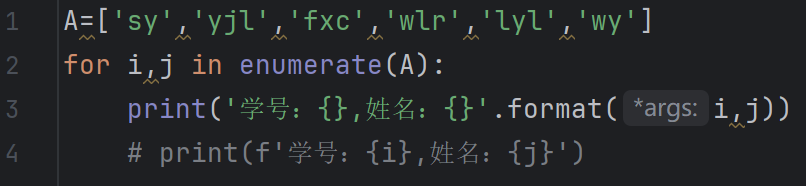
\includegraphics[width=\textwidth]{enumerate program1.png} % 确保图片宽度不超过页面宽度
        \caption{3.1.2.3}
        \label{fig:line-graph2}
    \end{subfigure}
    \hfill
    \begin{subfigure}[b]{0.35\textwidth}
        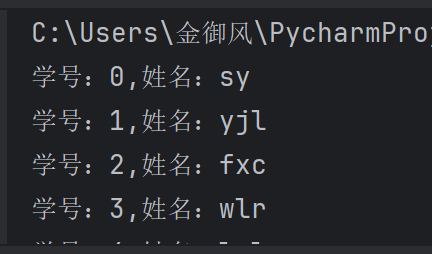
\includegraphics[width=\textwidth]{enumerate output1.png} % 确保图片宽度不超过页面宽度
        \caption{3.1.2.4}
        \label{fig:line-graph2-pic2}
    \end{subfigure}
\end{figure}
\noindent 注意注释掉的print也是对的,这是两种格式化字符串的方法,详见\ref{简写的使用规则}。第一个print中学号和姓名必须放在一个引号内,不能两个拼接,否则format只会对应后一个引号内的{},以及注意format()前是'.'不是','!

下面来看如何利用enumerate添加数值标签。
\begin{figure}[H]
    \centering
    \begin{subfigure}[b]{0.6\textwidth}
        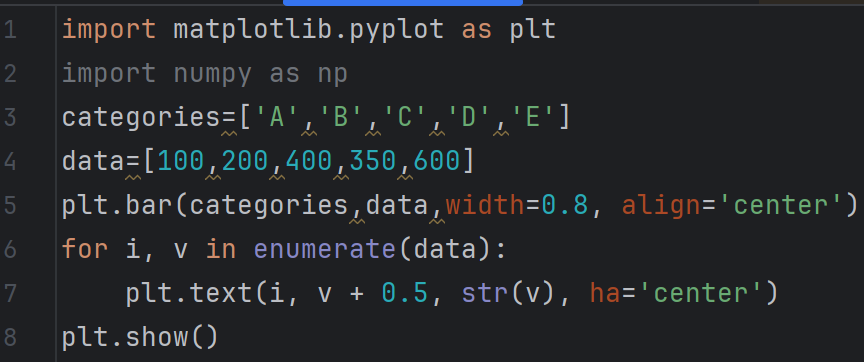
\includegraphics[width=\textwidth]{enumerate program2.png} % 确保图片宽度不超过页面宽度
        \caption{3.1.2.5}
        \label{fig:line-graph2}
    \end{subfigure}
    \hfill
    \begin{subfigure}[b]{0.38\textwidth}
        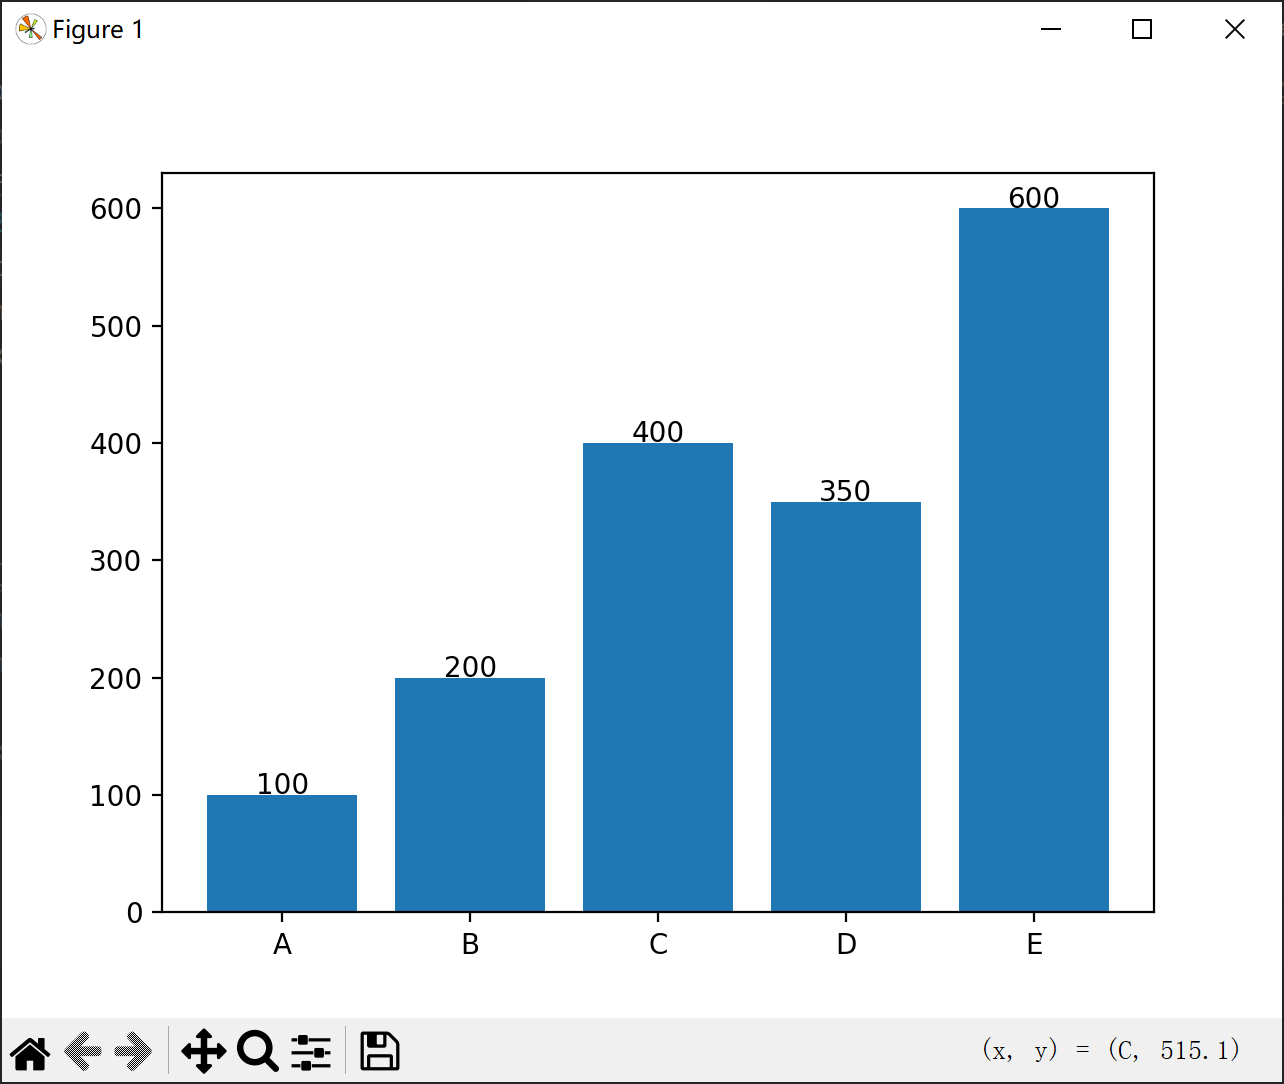
\includegraphics[width=\textwidth]{enumerate Pic2.png} % 确保图片宽度不超过页面宽度
        \caption{3.1.2.6}
        \label{fig:line-graph2-pic2}
    \end{subfigure}
\end{figure}
哎呀差点忘了说了,我们还要用到plt.text()函数,它的前两个参数是x,y坐标,我们令x=i是因为不同类间距恰好默认为1,而且第一类又是从x=0开始的(\textcolor{red}{这里要特别注意!!一般条形图原点是第一类标记处,不是图上看上去的横纵轴交点!}),这样每一类的标签正好可以落在类的正上方(以及条形的中央,因为align=’center‘),令v+0.5是为了让标签不与条形干涉,出现在稍靠上位置。第三个参数就是标签写些什么,这里是以数值本身作为标签,ha是horizontalalignment的简称,设定了标签文本在前面指定坐标的什么相对位置出现,可以是 'left'、'center'、'right'。

这个plt.text函数可以在图像的指定位置添加文本,是一个很有用的piplot函数,后面我们还要细讲它。\ref{text函数}

\noindent\textbf{水平条形图}

将bar()改为barh(),竖直条形图就变成了水平条形图,只需要做少许改动,首先是如果要设定宽度,参数是height而不是width,还要就是使用plt.text函数添加数值标签时x,y和竖直是反着的,别忘了交换。



\subsubsection{直方图}

直方图和条形图很像,区别是条形图是明确知道分为几类,每一类对应的数值是多少;而直方图则是已知一堆杂乱的数据,通过指定划分为多少类,分类范围,将这些数据按照数值大小分类,统计落在每一类的数据个数(或比例),比如下图3.1.4.1就是将60颗子弹的出膛速度绘制成了15类的直方图,其程序如图3.1.4.2。
\begin{figure}[H]
    \centering
    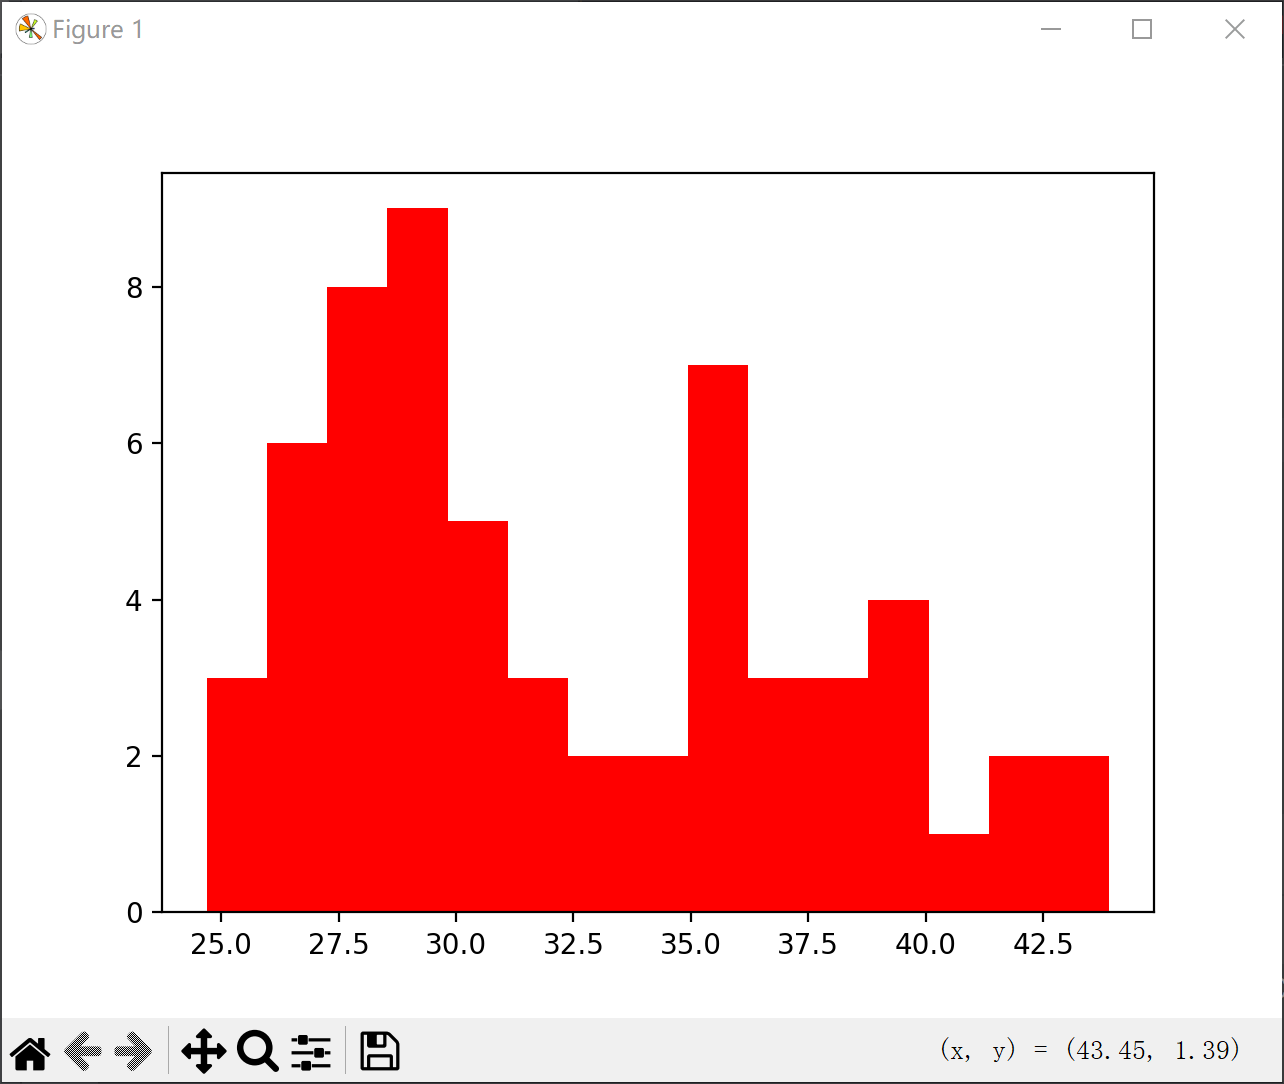
\includegraphics[width=0.8\linewidth]{直方图 Pic1.png}
    \caption{3.1.4.1}
    \label{fig:enter-label}
\end{figure}
\begin{figure}[H]
    \centering
    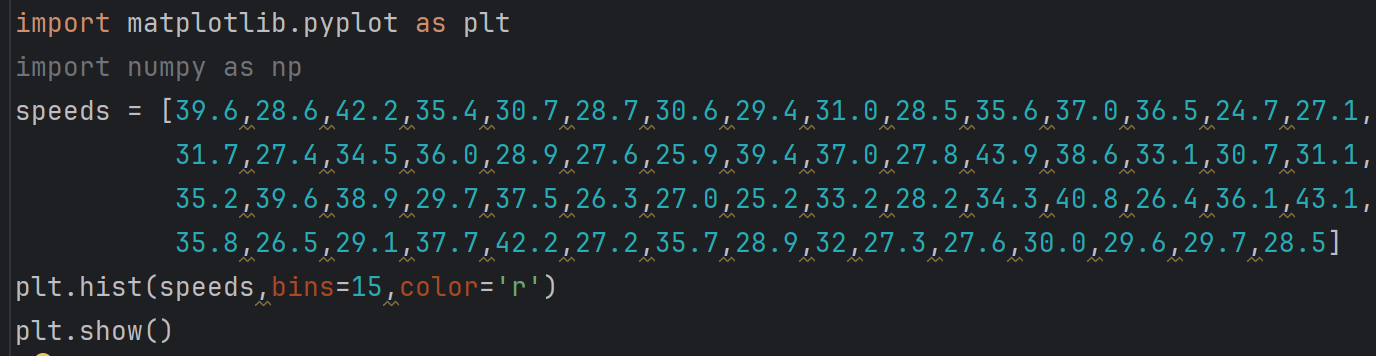
\includegraphics[width=0.75\linewidth]{直方图 program1.png}
    \caption{3.1.4.2}
    \label{fig:enter-label}
\end{figure}
plt.hist()函数接受的两个核心参数就是包含所有数据的列表(或一维numpy数组)和分的类数bins。此外就是我们熟悉的一下基本设置:color,edgecolor,alpha,不用多说了吧。

当然plt.hist()函数也有一些我们之前没提过的设置:

1. range:数据的最小值和最大值,决定了直方图的横轴范围。

2. density: 如果为True,则直方图的纵轴显示概率密度(就是频率啦)。如果为False,则显示频数。通常默认为False。

3. histtype: 直方图的类型,可以是 'bar'、'step'、'stepfilled' 等。个人感觉bar和stepfilled没什么区别,而bar又是默认的状态,因此这里就展示一下图3.1.4.1以step的形式呈现是什么样子。
\begin{figure}[H]
    \centering
    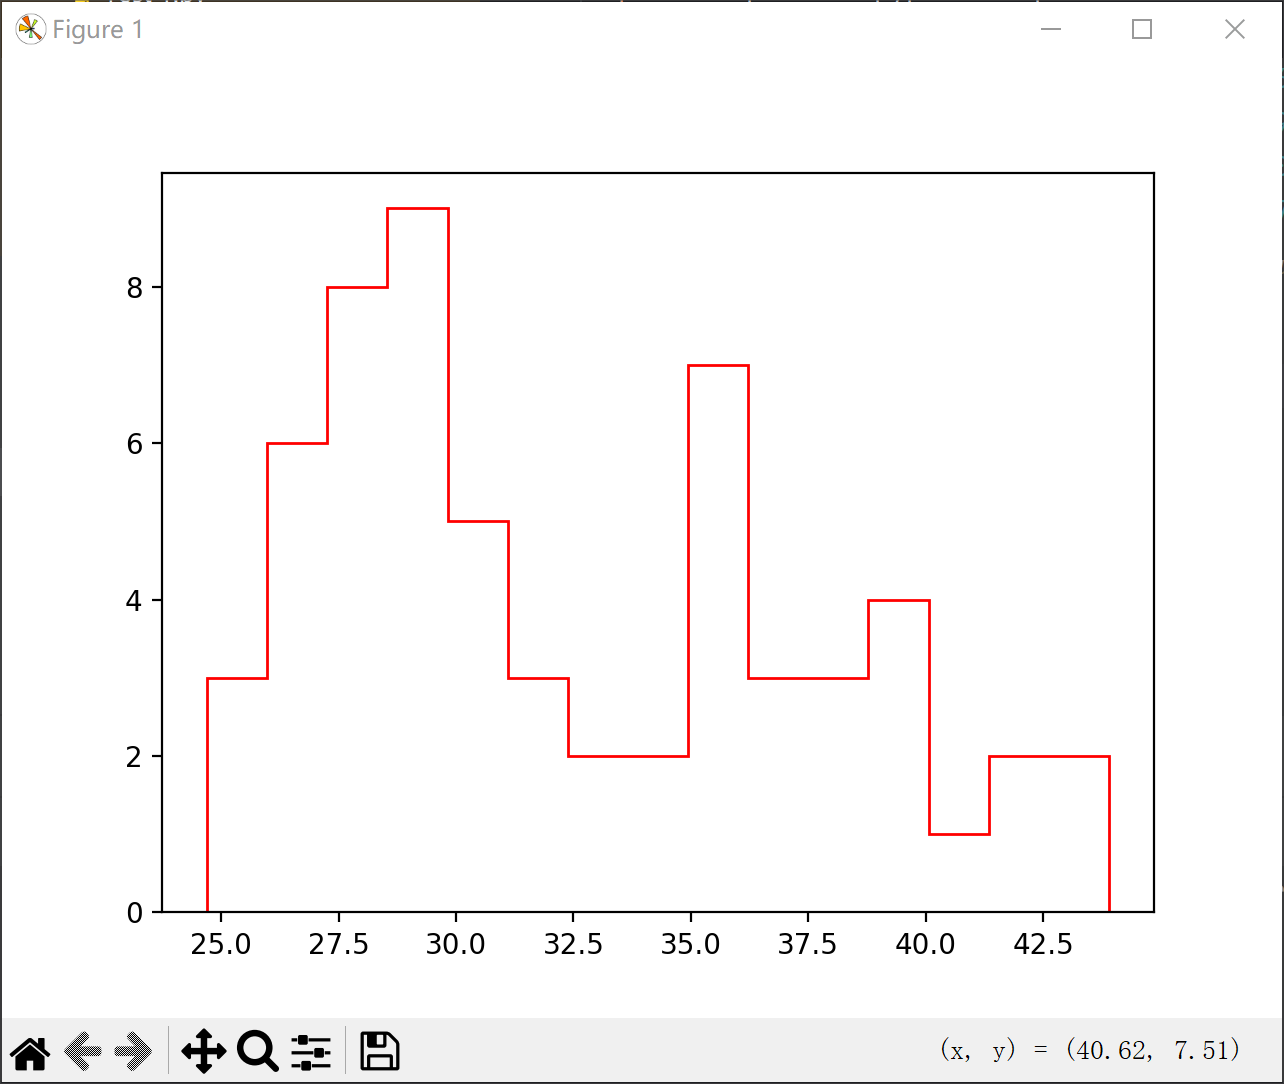
\includegraphics[width=0.5\linewidth]{直方图 Pic2.png}
    \caption{3.1.4.3}
    \label{fig:enter-label}
\end{figure}

4.cumulative: 为True时,显示的是每个 bin 加上所有之前 bin 的计数,相当于一个数据的逐渐累计,到最后一个bin,其计数应是数据总数。相应的,如果cumulative=True并且density=True,那么最后一个bin应该等于1。这种方法可以用来观察数据的累积分布情况。比如图3.1.4.1以cumulative=1的形式呈现如下:
\begin{figure}[H]
    \centering
    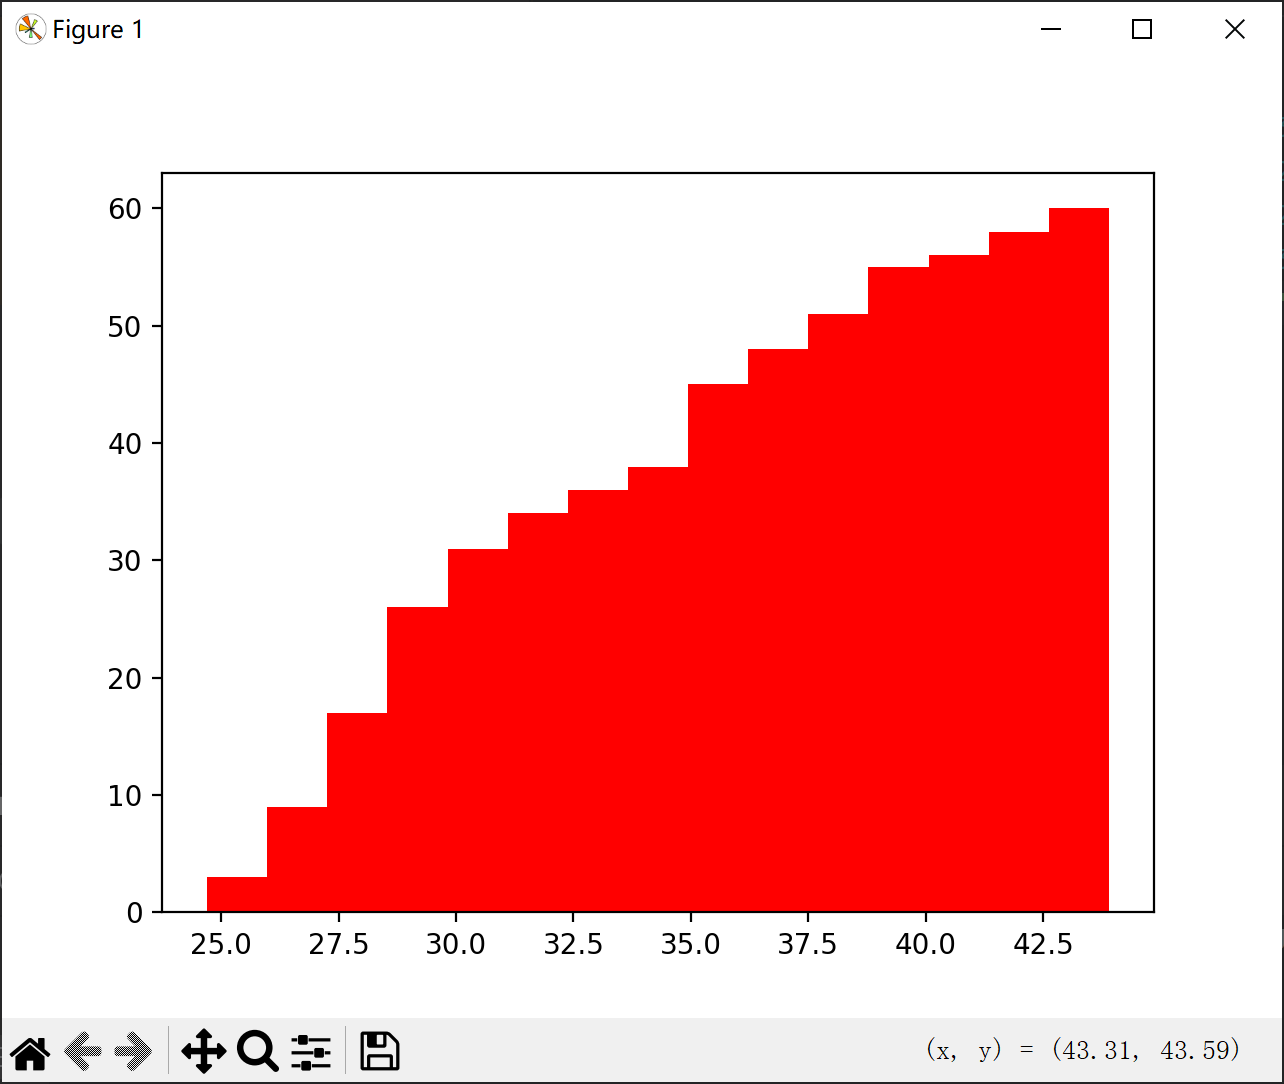
\includegraphics[width=0.5\linewidth]{直方图 Pic3.png}
    \caption{3.1.4.4}
    \label{fig:enter-label}
\end{figure}
除此之外,还有一些特殊的直方图,比如:
\begin{figure}[H]
    \centering
    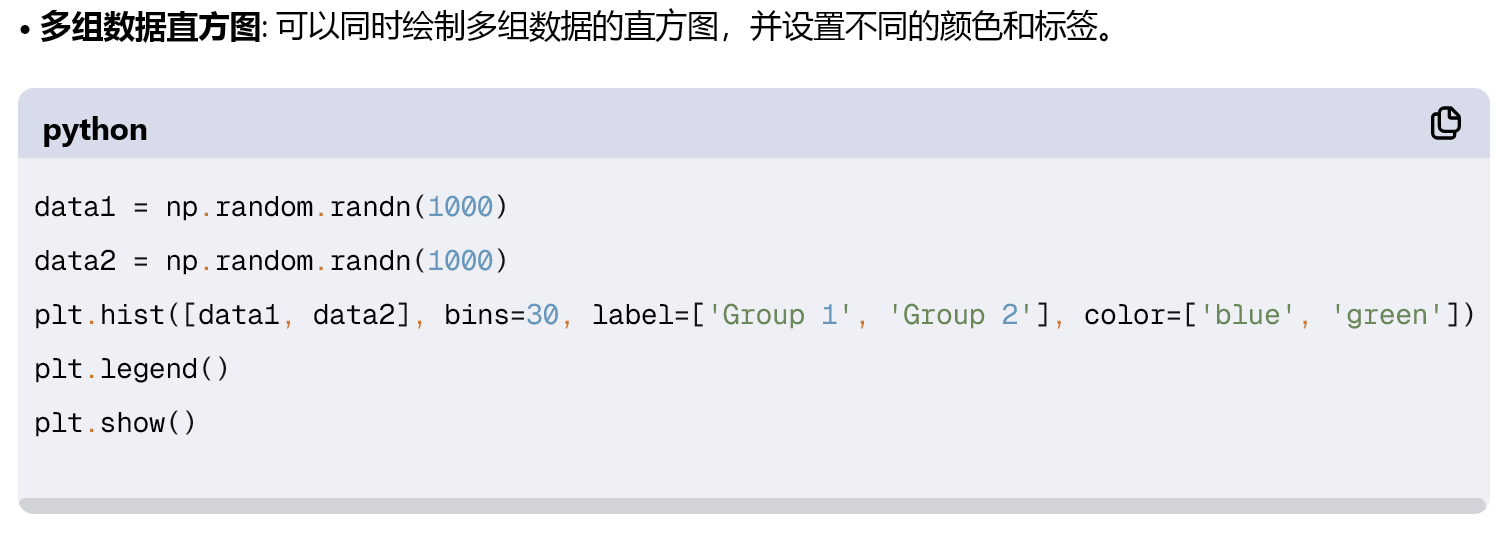
\includegraphics[width=1\linewidth]{直方图 program4.png}
    \caption{3.1.4.5}
    \label{fig:enter-label}
\end{figure}
\noindent 如果使用stacked=True参数还可以将多组数据的直方图堆叠在一起,就形成了堆叠直方图。总之,可以向hist()传递不止一个列表,让多组数据在一张图中呈现。

Pyplot绘图的基本方法到这里就结束了,其他特殊的Pyplot绘图方法放在\ref{Pyplot绘图的其他方法} 中简要介绍。
\subsection{Pyplot设置坐标轴的基本方法}
除了绘图,Pyplot还有一些设置坐标轴的方法,相比Axes设置坐标轴的方法,Pyplot的方法更简单,更基础,但是实现的功能也较为有限。
\subsubsection{xlim(),ylim()函数}
如果我们令plt.xlim((-1,2)),那么图像的定义域就会被限定在(-1,2)区间内,ylim同理,通常我们用元组形式表示这个限定区间(所以出现了双括号),但是其实plt.xlim(-1,2)也是可以的。
\subsubsection{xticks,yticks函数}
这是一个很有用的函数,能对坐标轴进行很多方面的设置。以xticks为例,其可接受的参数有:

\textit{\large plt.xticks(ticks,labels,minor,kwargs)}


其中ticks是对刻度的设置,注意它与xlim()的区别!ticks对坐标轴的限制仅是对有刻度区域的限制,以及对刻度形式的设置,其数据类型可以是numpy数组,列表及元组。比方说令ticks=[-2,-1,0,1,2],那么x轴虽然还是xlim()或者x=np.linspace规定的范围,但是只有-2,-1,0,1,2这五个地方会有刻度。(我们也有时用np.linspace生成ticks)labels应当是一个长度和ticks相同的列表或什么别的,它指定了那些标出来的刻度叫什么名字,因而需要与ticks中元素一一对应。

minor暂时没有发现有什么有用的功能,其作用似乎是:minor=True时,之前设置的ticks与label会被忽略,minor=False时则会正常显现设置效果。

这个kwargs其实是一些额外参数的统称,常用的包括color,fontsize(字体大小),rotation(字体旋转角度)等等。
 
\subsubsection{xlabel,ylabel函数}
用法就是plt.xlabel(' '),plt.ylabel(' '),用来指定x,y坐标轴的名字。

\subsubsection{grid函数}
用法是plt.grid(True)或者plt.grid(False),True的时候会根据刻度划分生成网格。

\subsubsection{title函数}\label{title函数}
这是用来设置图表标题的函数,其用法如下:

\textit{\large plt.title(label, fontdict, loc, pad)}

\noindent label用于指定图表的标题内容,是必须提供的参数。

\noindent fontdict用于设置标题的字体样式,如字体大小、字体颜色、字体类型等。它是一个字典,因此形如:fontdict={'fontsize': 14, 'color': 'red', 'fontweight': 'bold'}  可以设置标题的字体大小为14,颜色为红色,字体加粗。'red'这里可以简写,然后'fontweight'的可选值有:

1.   'light'  :较细的字体

2.   'normal'  :正常粗细的字体,也是默认值

3.   'medium'  :中等粗细的字体

4.   'semibold'  :半粗体

5.   'bold'  :粗体

6.   'heavy'  :较粗的字体

7.   'black'  :最粗的字体

\noindent loc 是标题的位置,可选值有 'center'  (居中,默认值)、  'left'  (左对齐)、  'right'  (右对齐),用于控制标题在图表顶部的水平位置。

\noindent pad是标题与图表顶部的间距,单位为点数(1点等于1/72英寸)。(个人觉得这个参数没什么用)

pyplot还有一个功能与之很相似的函数plt.subtitle(),它们的区别我们放在\ref{subtitle函数以及它和title的区别}里讲。
\subsubsection{axis函数}

plt.axis()虽然有很多参数,但是最好一个函数只接受一个参数,所以得分成多个plt.axis()来进行设置。其包含的参数有:

 \noindent 1. plt.axis([xmin, xmax, ymin, ymax])  :直接指定x轴和y轴的显示范围,其中  xmin  和  xmax  分别表示x轴的最小值和最大值,  ymin  和  ymax  分别表示y轴的最小值和最大值。

 \noindent 2. plt.axis('off')  :关闭坐标轴的显示,使图表中不显示坐标轴。其默认状态是on,一旦被设成‘off’,与坐标轴有关的其他设置也将不复存在。效果如下图:
 \begin{figure}[H]
     \centering
     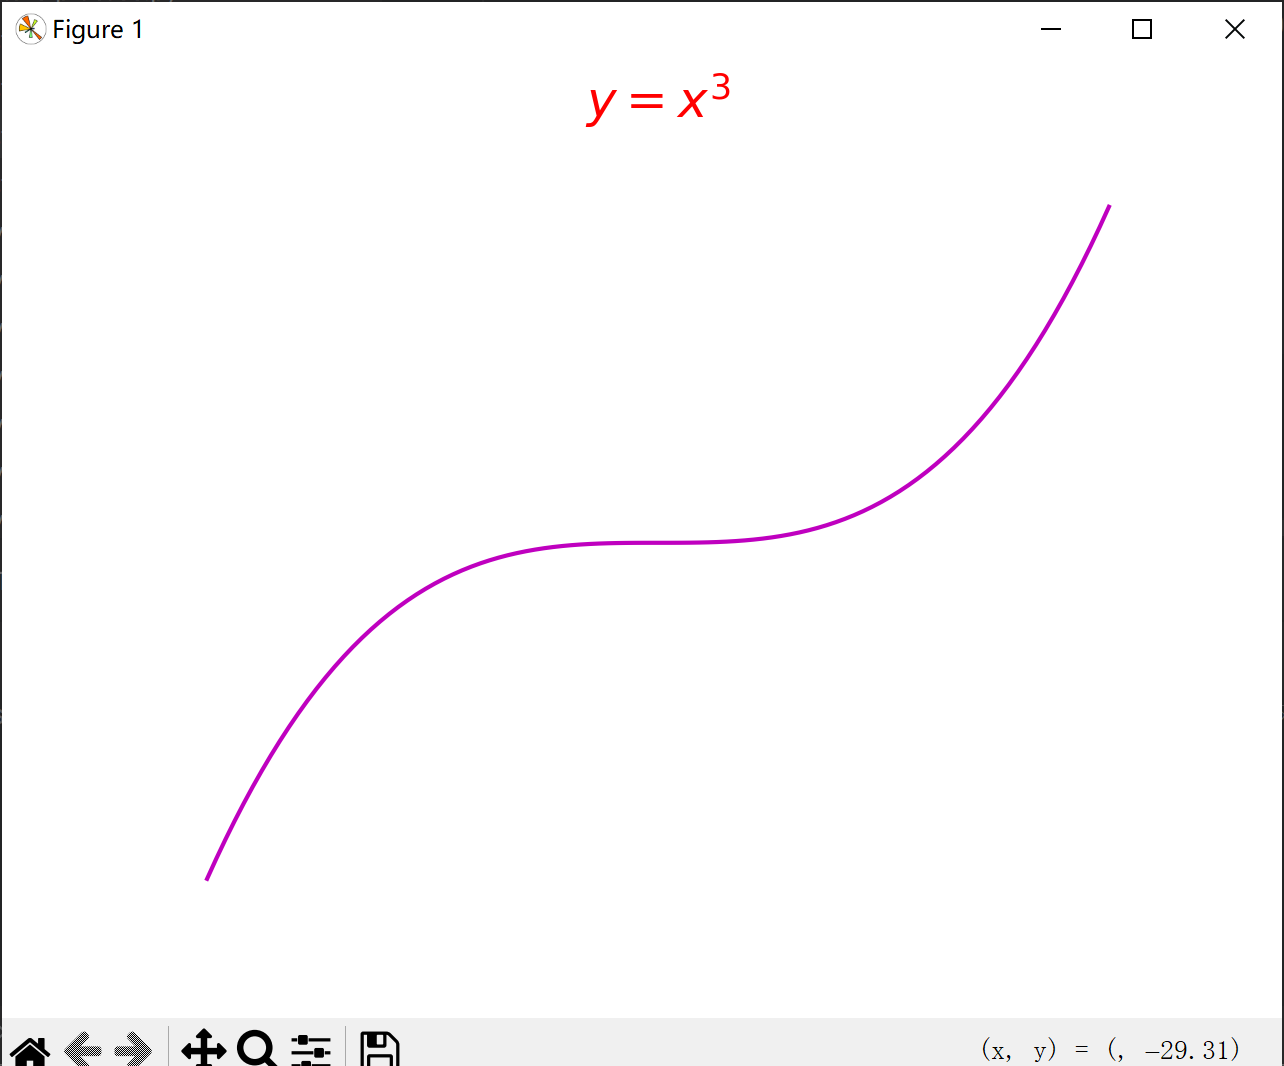
\includegraphics[width=0.45\linewidth]{pyplot坐标轴Pic2.png}
     \caption{3.2.6.1}
     \label{fig:enter-label}
 \end{figure}

 \noindent 3. plt.axis('equal')  :设置坐标轴的刻度间隔相等。  

\noindent 4. plt.axis('scaled')  :设置坐标轴的刻度间隔相等,并根据图表大小自动调整范围。

\noindent 5. plt.axis('tight')  :自动调整坐标轴范围,使数据紧密显示。





下面我们看一个融合了以上方法的示例:
 \begin{figure}[H]
     \centering
     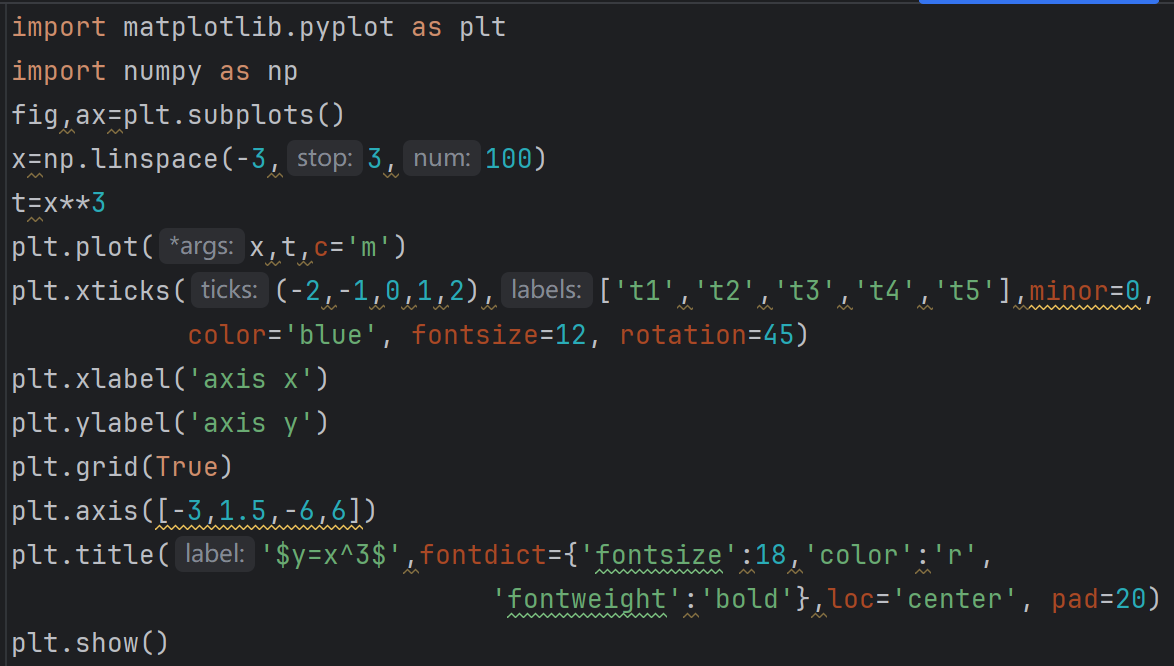
\includegraphics[width=0.9\linewidth]{pyplot坐标轴program1.png}
     \caption{3.2.2.1}
     \label{fig:enter-label}
 \end{figure}

\begin{figure}[H]
    \centering
    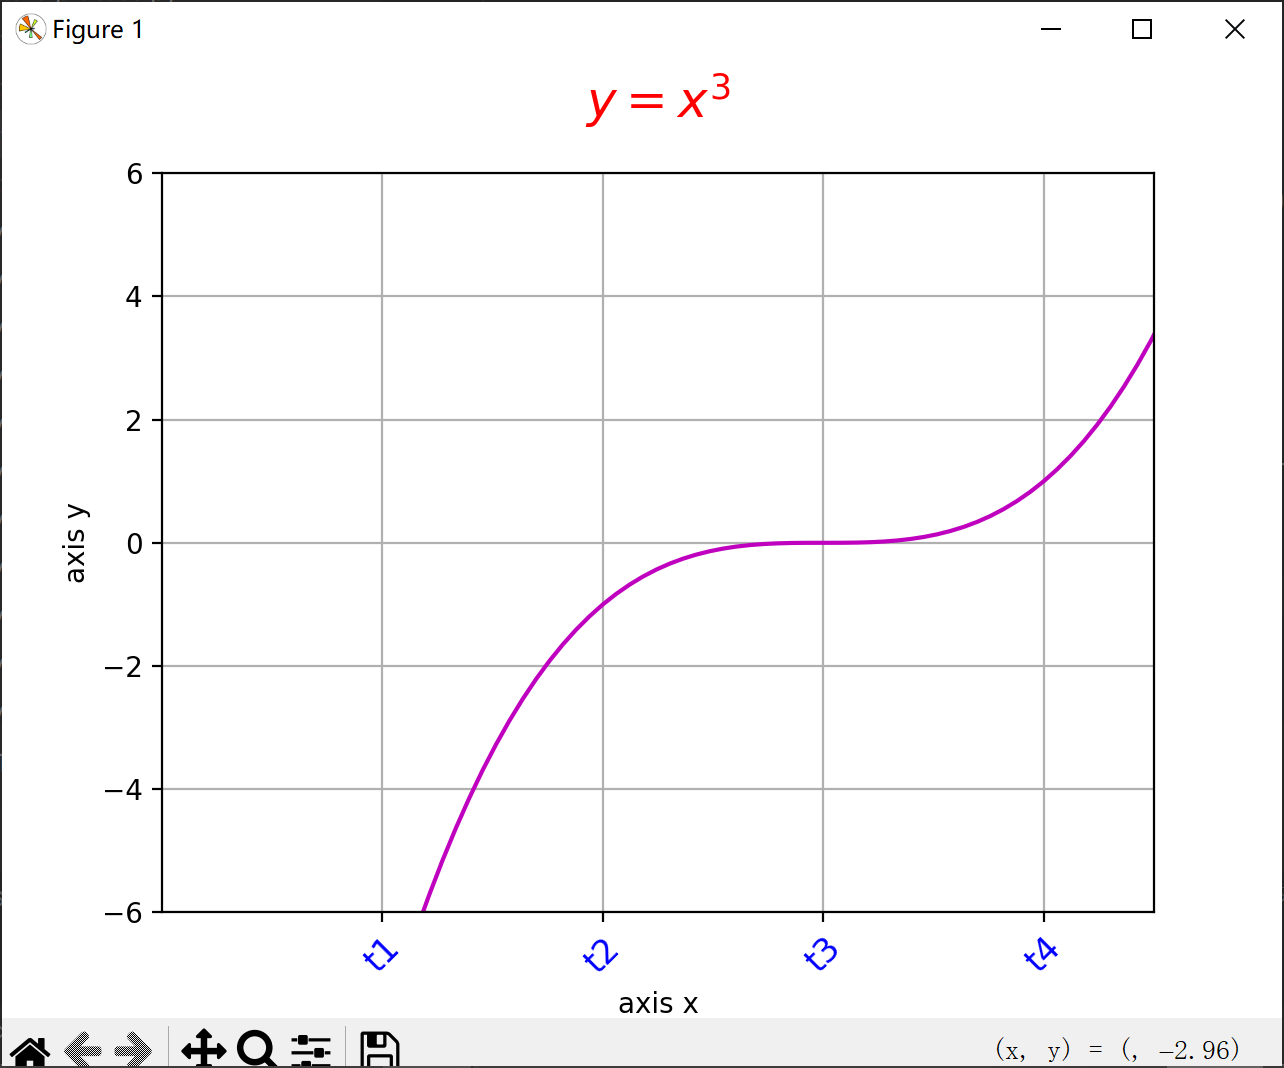
\includegraphics[width=0.65\linewidth]{pyplot坐标轴Pic1.png}
    \caption{3.2.2.2}
    \label{fig:enter-label}
\end{figure}

\subsection{在图中添加文本}
Pyplot中添加文本的函数主要有text,xlabel和ylabel,annotate,title和subtitle,其中title和xlabel、ylabel之前已经讲过,这里重点介绍另外几个。
\subsubsection{text函数}\label{text函数}
text的基本参数就是x,y坐标和内容,这我们之前就提到过,下面介绍其更复杂的设置。
\noindent\textbf{位置设置}

text函数设置文本位置的方法不止x,y坐标一种,我们来看一个不用坐标的例子:

\[plt.text(0.5, 0.5,\, 'Center\, of\, Axes',\, transform=ax.transAxes)\]
在这个例子中出现了一个新的参数transform,它用来指定设置位置所用的坐标系,或者说采用的参考方式,常用的坐标系有:

1.   ax.transData  :数据坐标系(默认值),就是在子图中的x,y坐标。

2.   ax.transAxes  :轴坐标系,范围是 0 到 1,其中 (0,0) 是轴的左下角,(1,1) 是轴的右上角,就是在子图中的相对位置,或者说分别相对于x,y坐标轴的位置。

3.   fig.transFigure  :图形坐标系,范围也是 0 到 1,是相对于整个图形窗口的位置。

因此,上述例子中是将文本放置在了两轴的中心位置。

(注意前面有ax.或fig.,所以别忘了提前创建坐标轴或图形对象)

\noindent\textbf{文本内容设置}

内容其实没什么好说的,就说两点:一是如果文本不止一行,可以使用使用换行符\textbackslash{}n ,例如plt.text(1, 2, 'Line 1\textbackslash{}nLine 2')   
还有一点就是text以及matplotlib其它添加文本的方式一般都是添加英文文本的,如果要添加中文的话,最简单的做法是在前面添上两行代码:
\[plt.rcParams['font.sans-serif'] = ['SimHei']\]
\[plt.rcParams['axes.unicode\_minus'] = False \]
(不用导入别的什么包,看来pyplot还是太全面了)

\noindent\textbf{字体和样式设置}

1. fontsize:设置文本的字体大小。可以是数值,也可以是预定义的大小名称,如   'small'  、  'medium'  、  'large'   等。


2. fontweight:设置字体的粗细。常见的值有   'normal'  、  'bold'  、  'light'   等。

3. 例如,  plt.text(1, 2, 'Bold Text', fontweight='bold')  。

4. fontstyle:设置字体的风格。常见的值有   'normal'  、  'italic'  、  'oblique'   等。

5. color:设置文本的颜色。可以是颜色名称(如   'red'  、  'blue'   等),也可以是十六进制颜色代码(如   '\#FF0000'  )。


6. family:设置字体家族。常见的值有   'serif'  、  'sans-serif'  、  'cursive'、   'fantasy'、  ‘monospace’ 等。

这个字体家族控制的是文本的总体风格,可能有些难以理解,下面用以下代码展示不同字体家族的效果:
\begin{figure}[H]
    \centering
    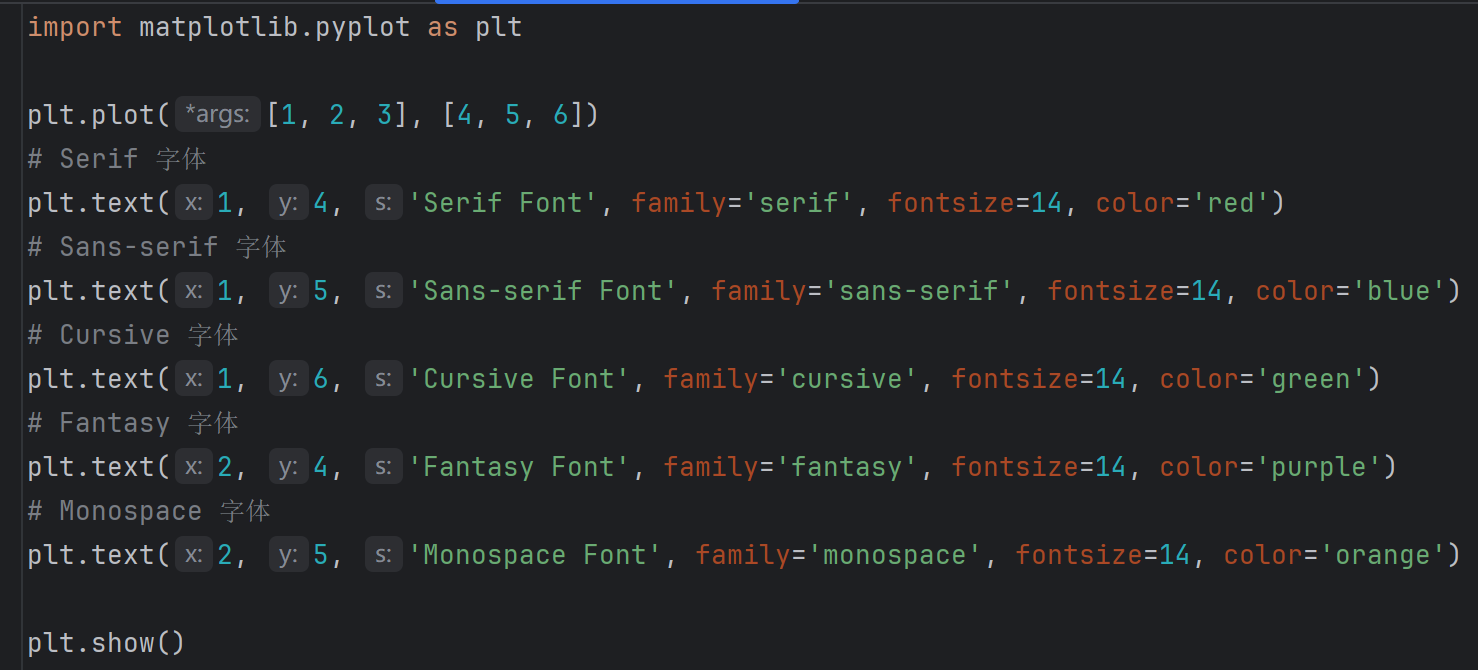
\includegraphics[width=0.75\linewidth]{字体家族 program.png}
    \caption{3.3.1.1}
    \label{fig:enter-label}
\end{figure}

\begin{figure}[H]
    \centering
    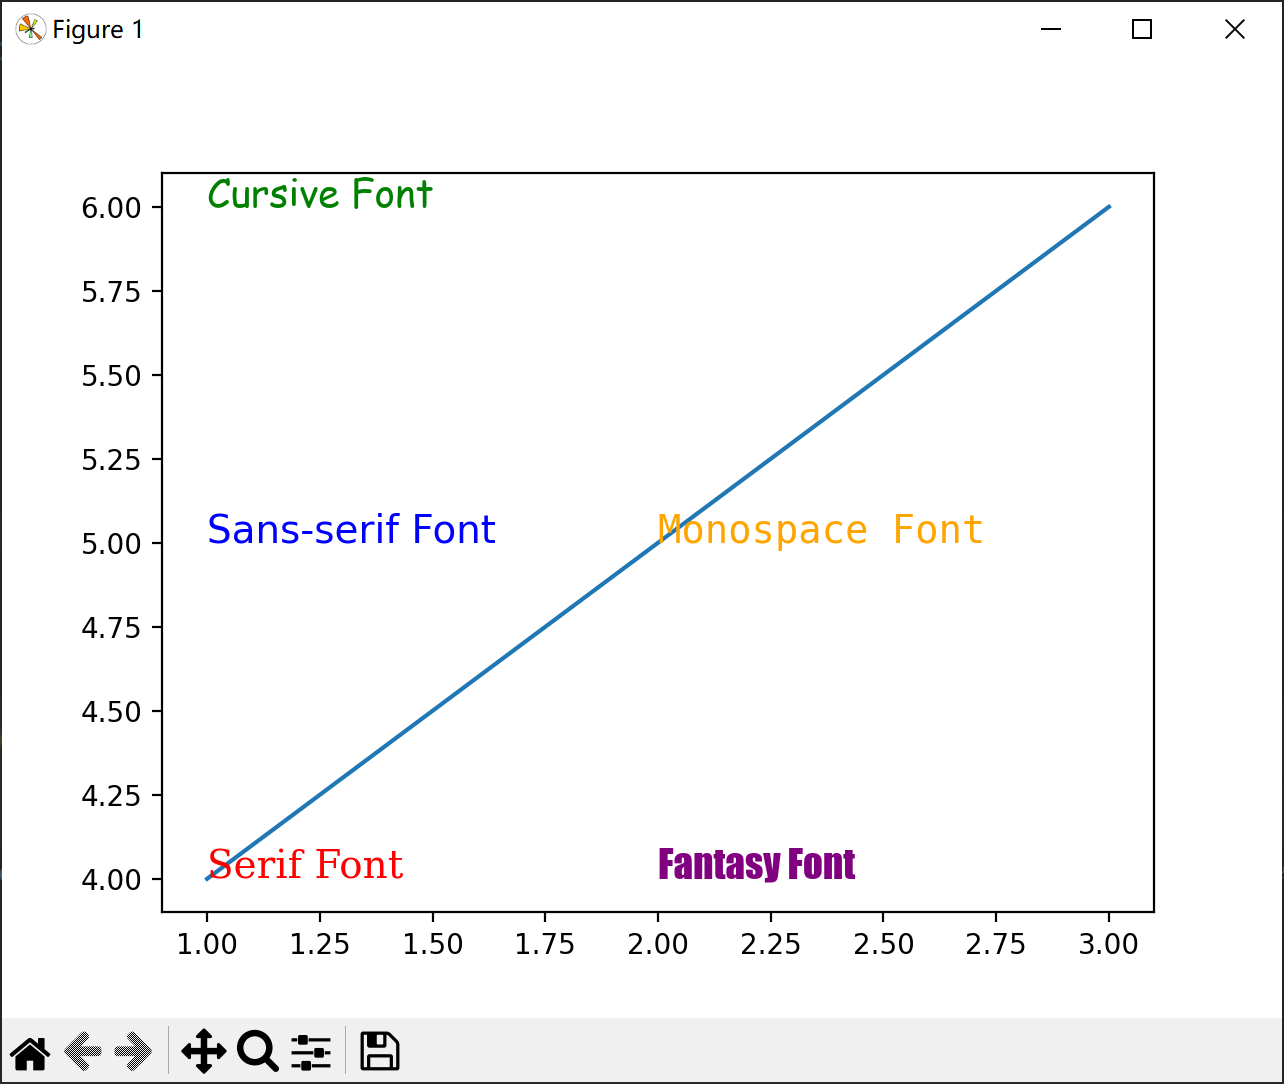
\includegraphics[width=0.65\linewidth]{字体家族 Pic.png}
    \caption{3.3.1.2}
    \label{fig:enter-label}
\end{figure}

\subsubsection{subtitle函数以及它和title的区别}\label{subtitle函数以及它和title的区别}
二者最本质的区别是title用于设置单个子图(axes)的标题,而subtitle用于设置整个图形对象(fig)的总标题。对于多子图的fig,title设置的标题仅对一个子图有效,不会影响其他子图;而无论图形中有多少个子图,  suptitle()   添加的标题都只有一行,它覆盖整个图形的顶部区域。

二者的设置参数都一样,参考\ref{title函数},只不过因为是总标题,subtitle字体的默认大小会大一些。

\subsubsection{annotate函数}
annotate函数的功能是在图中添加带箭头的注释文本,其用法和主要参数如下:
\[plt.annotate(\,'\;',\,xy=(\,),\,xytext=(\,),\,arrowprops=\{\,'arrowstyle'\,:\, '\;',\, 'color'\,:\, '\;',\,'lw':\;\;\})\]

第一个引号内容为注释文本,xy接受的是箭头指向的坐标元组,xytext接受的是注释文本所在位置的坐标(默认似乎是左对齐),arrowprops接受一个与箭头属性有关的字典,我们可以在这个字典中设置箭头的样式、颜色、宽度等。颜色和宽度就不用多说了,样式可以有一下选项:

1. '-'  :没有箭头,仅一条线。

2.   '->'  :简单的箭头,箭头指向右侧。

3.   '<-'  :简单的箭头,箭头指向左侧。

4.   '<->'  :双向箭头。

5.   '-['  :方括号箭头,箭头指向右侧。

6.   ']-'  :方括号箭头,箭头指向左侧。

7.   '-|>'  :带有垂直线的箭头,箭头指向右侧。

8.   '<|-|>'  :带有垂直线的双向箭头。

9.   'fancy'  :花哨的箭头,箭头指向右侧。

10   'simple'  :简单的箭头,箭头指向右侧。

11.   'wedge'  :楔形箭头,箭头指向右侧。

我们用如下程序展示这11种箭头:
\begin{figure}[H]
    \centering
    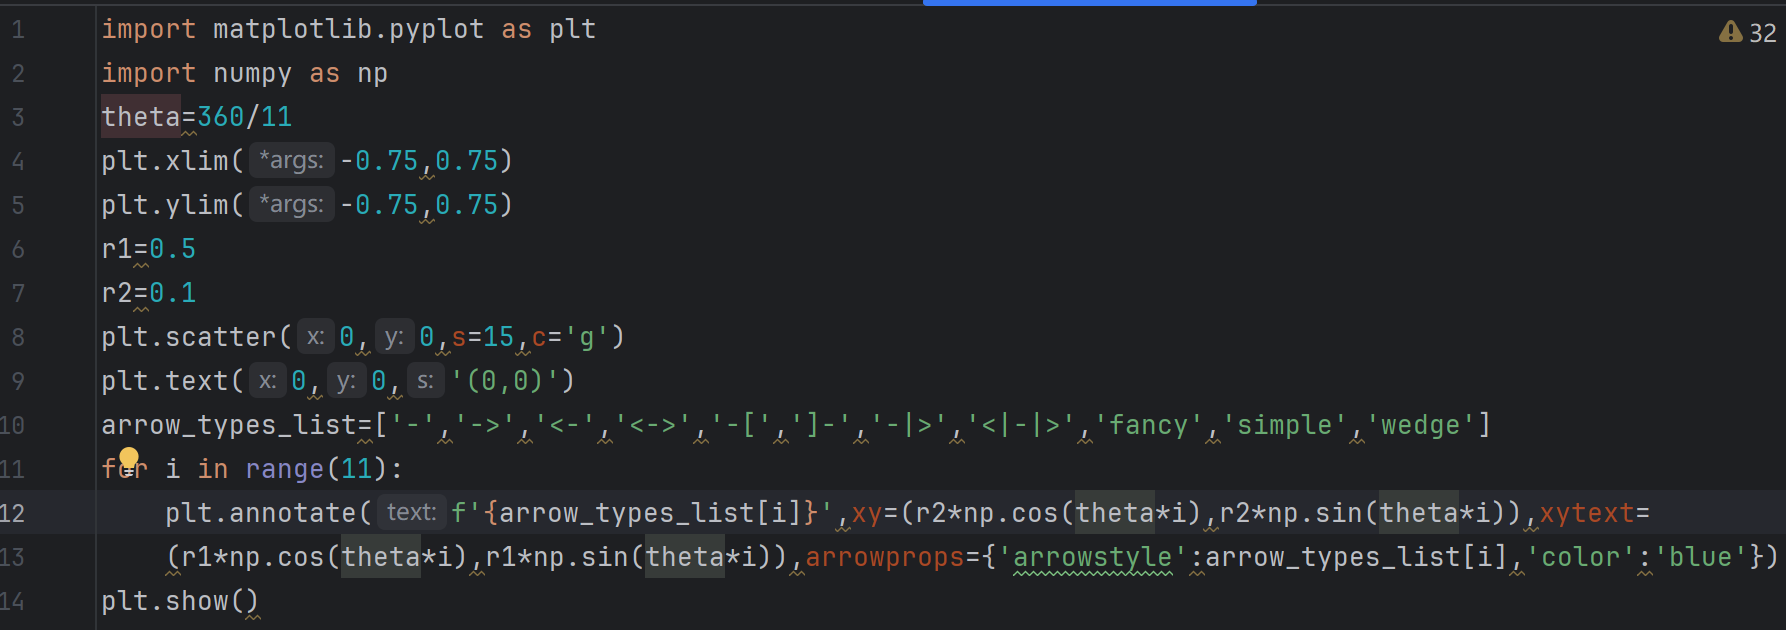
\includegraphics[width=1\linewidth]{annotate program1.png}
    \caption{3.3.3.1}
    \label{fig:enter-label}
\end{figure}

\begin{figure}[H]
    \centering
    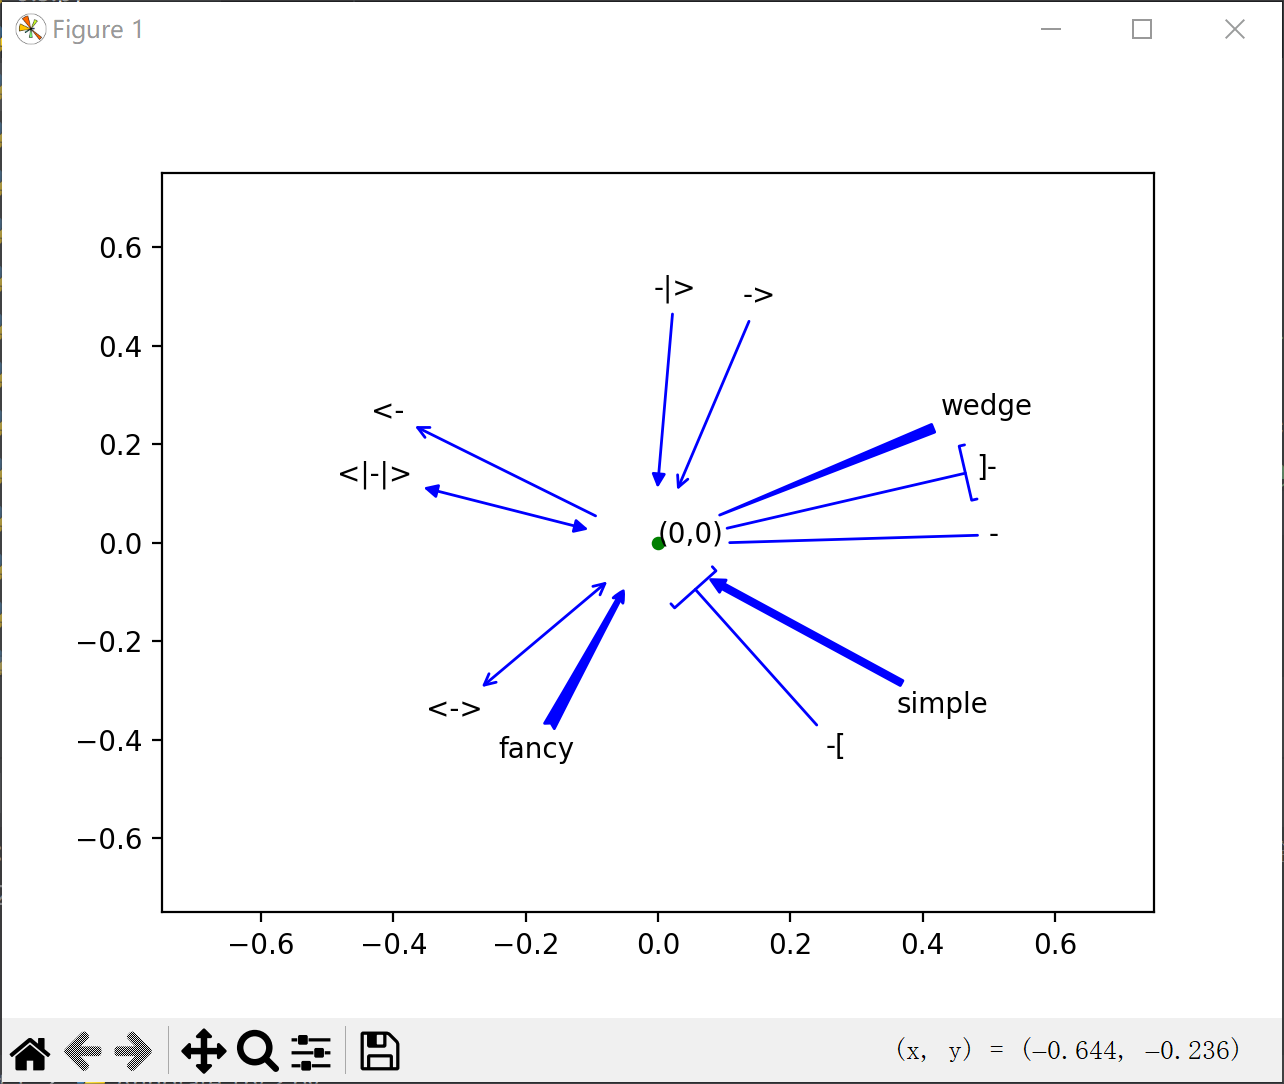
\includegraphics[width=0.6\linewidth]{annotate Pic1.png}
    \caption{3.3.3.2}
    \label{fig:enter-label}
\end{figure}




\section{Axes的基本用法}
\subsection{创建Axes对象}\label{创建Axes对象}
创建Axes对象(活跃坐标轴)的方法有一下几种,其中有一些还是pyplot的方法,我们会以在一个图形窗口绘制四张子图,分别是对数函数、指数函数、正弦函数,余弦函数为例,展示如何使用直线方法:
\begin{figure}[H]
    \centering
    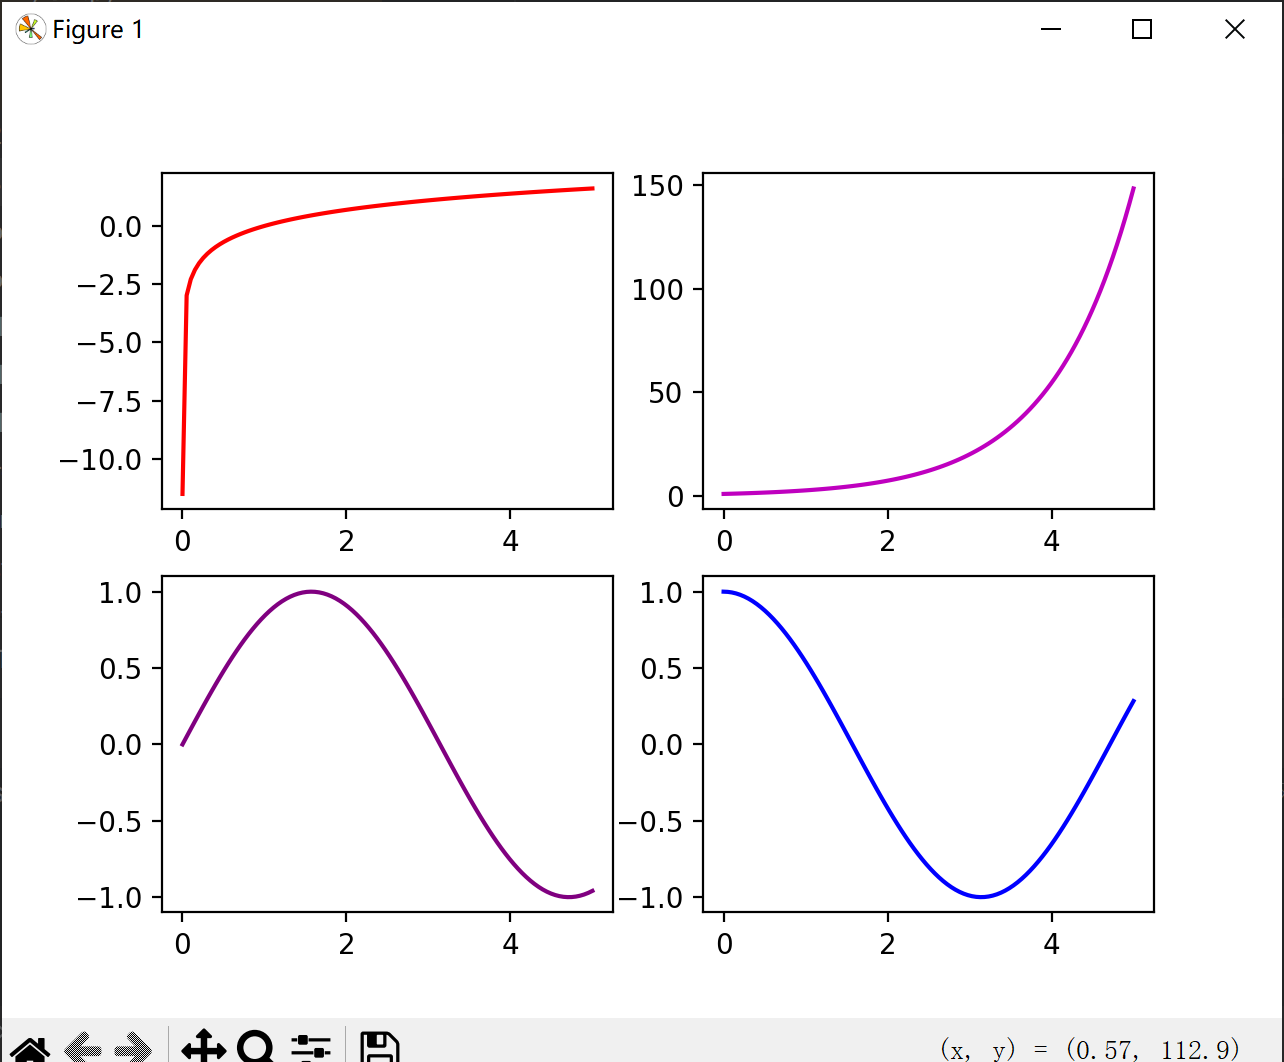
\includegraphics[width=0.5\linewidth]{创建子图 Pic1.png}
    \caption{4.1.1}
    \label{fig:enter-label}
\end{figure}

\noindent\textbf{\large 1. plt.subplot:}

\textit{plt.subplot(nrows, ncols, index)}

nrows, ncols是指这个方法将图形窗口分割成nrows行ncols列的网格,index则是对这个网格的索引,在index指定的位置创建一个子图。它的返回值是ax(一个子图)。

如果我们要在一个图形窗口绘制四张子图,分别是对数函数、指数函数、正弦函数,余弦函数,用plt.subplot方法是这样的:
\begin{figure}[H]
    \centering
    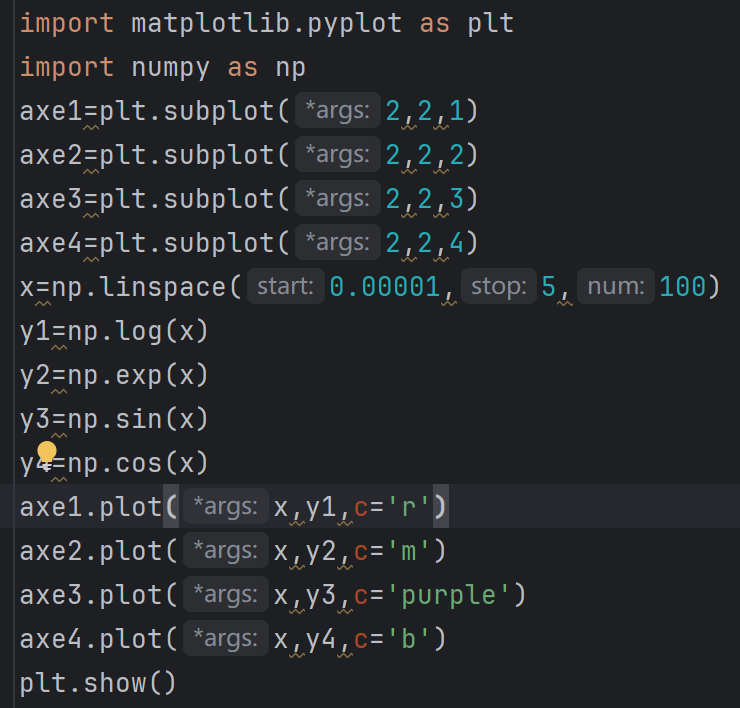
\includegraphics[width=0.65\linewidth]{创建子图 program1.png}
    \caption{4.1.2}
    \label{fig:enter-label}
\end{figure}
你也许会觉得这段代码很冗长,但是借助列表与遍历,我们可以对其进行简化:
\begin{figure}[H]
    \centering
    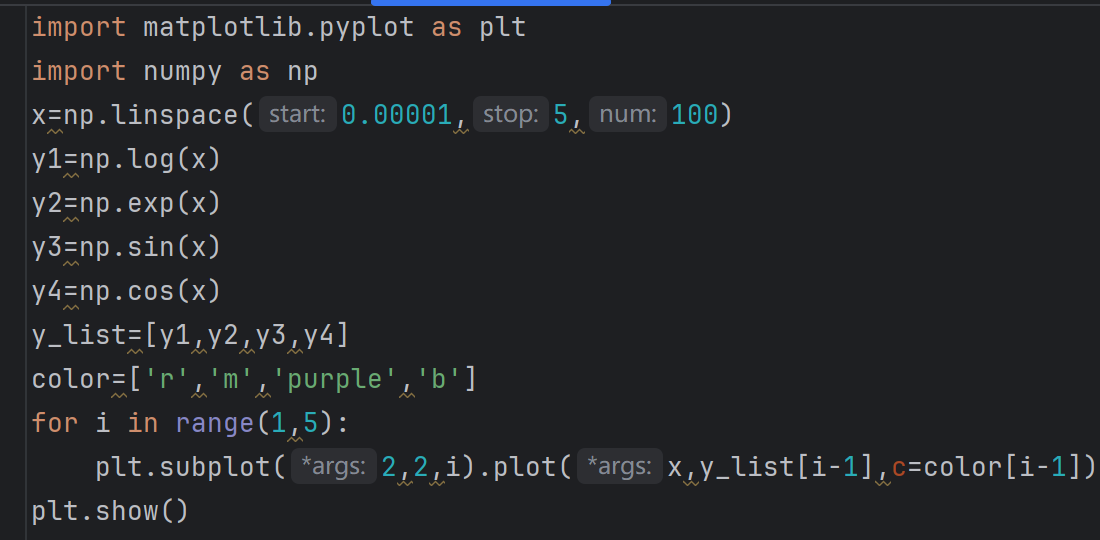
\includegraphics[width=0.75\linewidth]{创建子图 program1。2.png}
    \caption{4.1.3}
    \label{fig:enter-label}
\end{figure}
在\textit{plt.subplot(2,2,i).plot(x,y\_list[i-1],c=color[i-1])},我直接对刚刚创建出来的子图进行绘图操作,这种做法的可行,也佐证了我们之前提到的,pyplot方法支持链式调用。


\noindent\textbf{\large 2. plt.subplots:}

\textit{fig, ax = plt.subplots(nrows, ncols)}

和plt.subplot不同的是,(\textcolor{red}{注意!它们只有一个s之差!!})subplots不指定索引,因为它的返回值是图形对象fig和四个子图的集合,这个集合是一个二维数组(当nrows和ncols均大于一时),我们可以用[i,j]的形式来索引它,从而指定在不同位置的子图应该画什么图像。
如果我们只要画一幅子图,我们也可以直接令fig,ax = plt.subplots(),这样默认只创建应该子图,非常简便。

在这个示例(4.1.4)中,我作了两幅内容一样的图,区别是第二段代码明显更为简约,同时在第二段代码中我令sharex和sharey均等于True,指的是令x和y轴都共享,这样的效果如下图所示:
\begin{figure}[H]
    \centering
    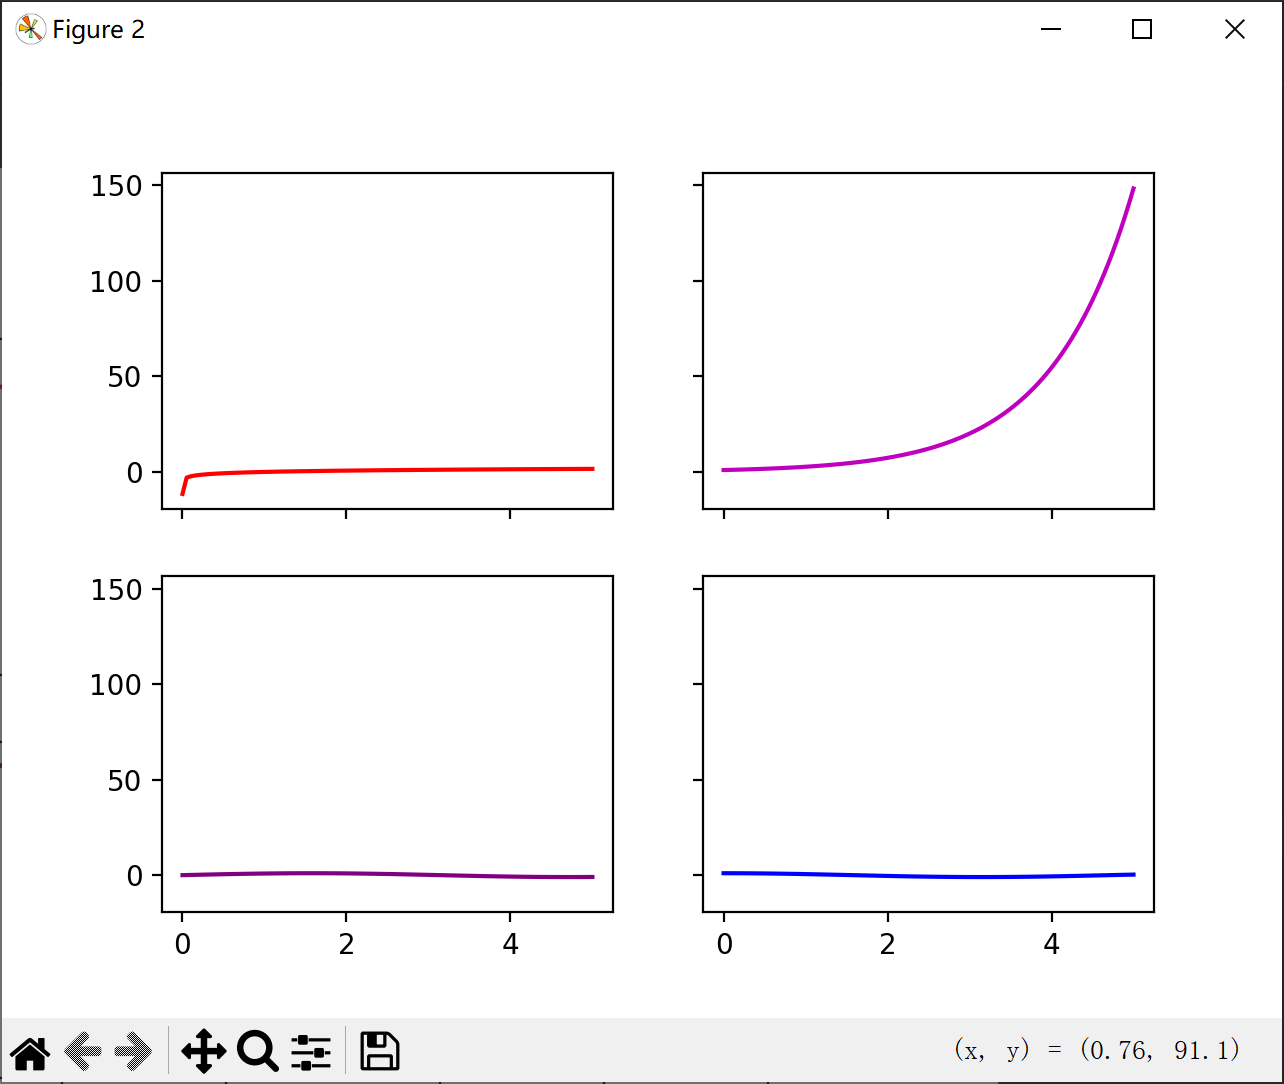
\includegraphics[width=0.45\linewidth]{创建子图 Pic2.png}
    \caption{4.1.5}
    \label{fig:enter-label}
\end{figure}
是不是感觉很难看?所以首先我们一般不会一下共享两个坐标轴,其次共享坐标轴是为了方便比较不同子图中数据的大小关系,一般不会用到它。
\begin{figure}[H]
    \centering
    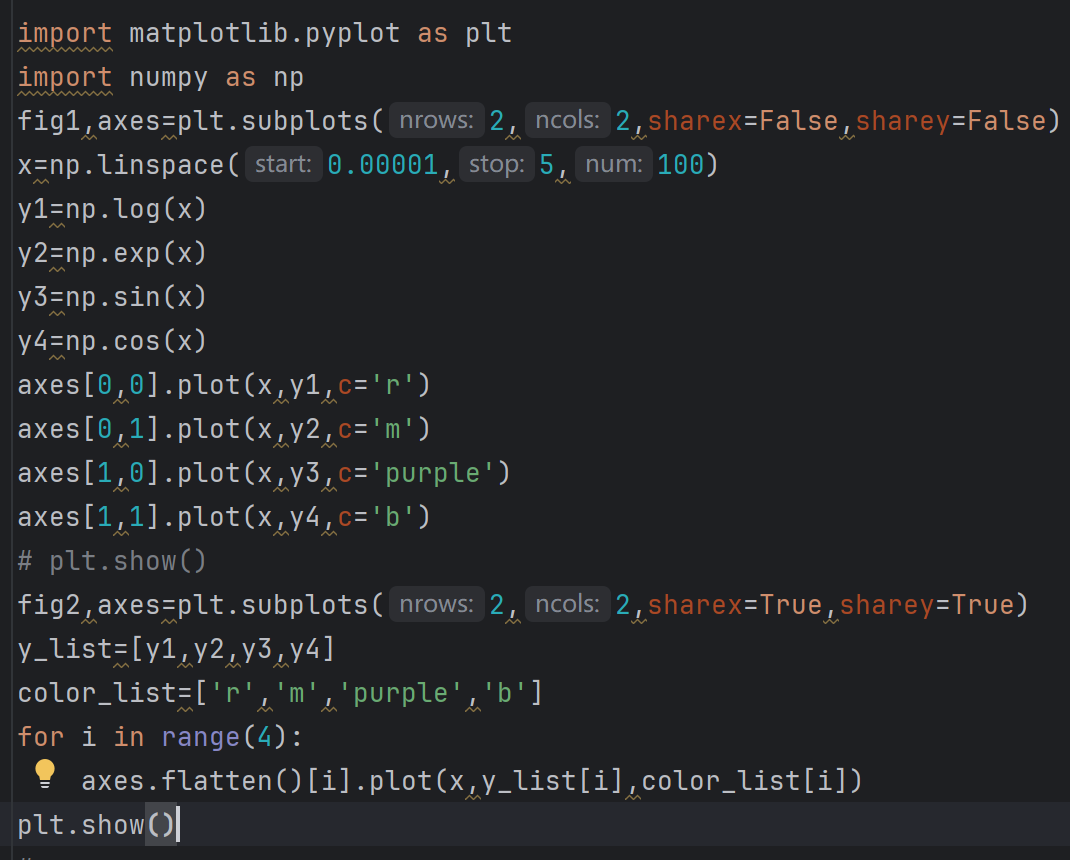
\includegraphics[width=0.75\linewidth]{创建子图 program2.png}
    \caption{4.1.4}
    \label{fig:enter-label}
\end{figure}
(还有一个很无聊的,你可注意可不注意的点,我在中间注释掉了一个plt.show(),这时两幅图是一起出现的,分别为Figure1和Figure2,但如果不注释掉,它会先出现Figure1,当你叉掉它后(专业一点说,终止掉Figure1的运行),Figure2才会出现(开始执行))


\noindent\textbf{\large 3. add\_subplot:}

\textit{fig.add\_subplot(nrows, ncols, index)}

这个方法是先创建图形对象fig,然后在这个图形对象基础上在index指定位置创建子图。要论它与方法1 plt.subplot()的区别,就是方法1更便捷快速,通常用于快速创建单个子图,而 fig.add\_subplot 允许你在已经创建的图形对象上添加子图。

\noindent\textbf{\large 4. add\_axes:}

\textit{fig.add\_axes([left, bottom, width, height])}

与add\_subplot相似的是,它也是先创建图形对象fig,然后在指定位置添加子图,不同的是,这个位置是通过left, bottom, width, height来指定的。
  add\_axes()   方法的参数是一个包含四个值的列表或元组,分别表示   Axes   对象的左下角的 x 坐标、y 坐标以及宽度和高度,这些值都是相对于图形窗口的大小的比例值(范围在 0 到 1 之间)。也就是说,它允许你指定   Axes   对象的确切位置和大小。

  \begin{figure}[H]
      \centering
      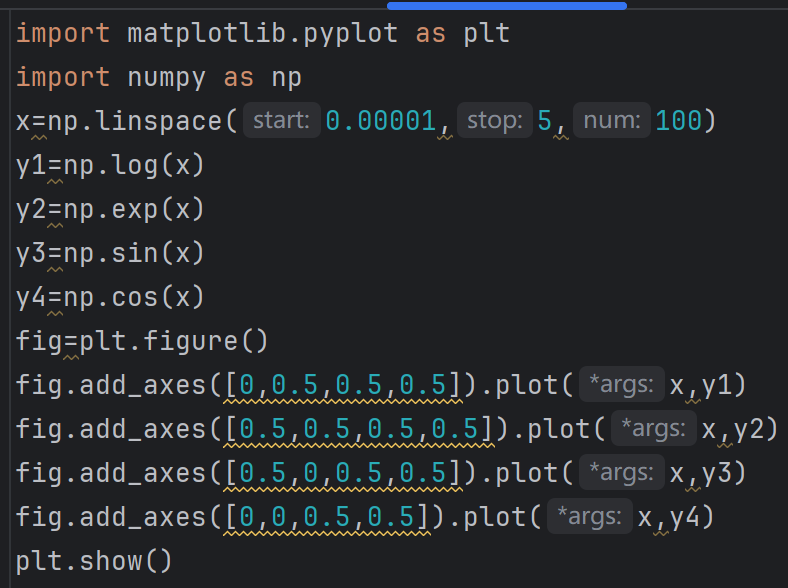
\includegraphics[width=0.75\linewidth]{创建子图 program3.png}
      \caption{4.1.5}
      \label{fig:enter-label}
  \end{figure}
我们之前说过,创建图形对象最简单的方式是plt.figure(),但是使用axes方法基本上都是ax.+函数的模式,就是说,你得先有函数可以作用的ax,也就是子图(坐标轴),这就需要用到上面介绍的四种创建子图的方法。比较这四种方法,我们发现:方法3和方法4都需要提前创建图形对象fig,而方法1和方法2都不需要,其中方法2是将图形对象fig和子图ax一起创建了,而方法1是完全不需要创建图形对象(毕竟人家是plt的方法嘛,在无图形对象的情况下创建子图,系统会自动生成一个图形对象)。总之我想说的是,如果需要用到axes的方法,我们需要结合实际需要,选择合适的创建子图的方法。

下面谈谈我自己的一些思考:我认为方法3是可以首先舍弃的,因为其功能和方法1其实完全一致,而没有方法1简便,因为它有依赖于图形对象的局限性。你也许想问,这个图形对象重要吗,一定要创建它吗;well,可以说在大多数时候,它是没什么用的,整段代码根本不需要它的存在;但是在少数时候它是必要的,比如说需要调整图形对象的长宽(就是生成出来的图像的大小),还有后面会将的事件处理与交互。所以,如果用不着创建图形对象,我们可以放心大胆地用方法1,如果子图又只有一张,那甚至可以效仿方法2的做法,直接简写为 ax=plt.subplot(),很简单吧。如果需要图形对象的话,我们通常可以采用方法2,将图形对象fig和子图ax一起创建了,即 fig,ax=plt.subplots()。方法4较为复杂,而且同样需要先创建figure,我认为其唯一用武之地就是需要专门设置不同子图在一张figure中的位置和大小的情况,这一点其他3个方法都代替不了。  

差点忘了说了,跳过figure直接创建ax其实还有一种方法,ax=plt.gca()。(怎么样够简单吧)
\newpage
\subsection{简述Pyplot和Axes的区别}

Pyplot和Axes的方法有许多是重合的,其唯一区别就是把plt换成了ax(或者别的名字,看你怎么定义的),如下表所示:

% Please add the following required packages to your document preamble:
% \usepackage{multirow}
\begin{table}[H]
\centering
\begin{tabular}{|c|c|c|c|}
\hline
类型                     & Pyplot                        & Axes                          & 功能           \\ \hline
\multirow{11}{*}{常规绘图} & plot(x, y, ...)               & plot(x, y, ...)               & 线图           \\ \cline{2-4} 
                       & scatter(x, y, ...)            & scatter(x, y, ...)            & 点图           \\ \cline{2-4} 
                       & bar(x, height, ...)           & bar(x, height, ...)           & 垂直条形图        \\ \cline{2-4} 
                       & barh(y, width, ...)           & barh(y, width, ...)           & 水平条形图        \\ \cline{2-4} 
                       & hist(x, bins, ...)            & hist(x, bins, ...)            & 直方图          \\ \cline{2-4} 
                       & boxplot(x, ...)               & boxplot(x, ...)               & 箱型图          \\ \cline{2-4} 
                       & fill\_between(x, y1, y2, ...) & fill\_between(x, y1, y2, ...) & 两曲线间填充颜色  \\ \cline{2-4} 
                       & step(x, y, ...)               & step(x, y, ...)               & 阶梯图          \\ \cline{2-4} 
                       & stem(x, y, ...)               & stem(x, y, ...)               & 茎叶图          \\ \cline{2-4} 
                       & pie(x, ...)                   & pie(x, ...)                   & 饼图           \\ \cline{2-4} 
                       & stackplot(x, y, ...)          & stackplot(x, y, ...)          & 堆积面积图        \\ \hline
\multirow{2}{*}{文本和注解} & text(x, y, s, ...)            & text(x, y, s, ...)            & 在图表中添加文本     \\ \cline{2-4} 
                       & annotate(xy, xytext, ...)     & annotate(xy, xytext, ...)     & 添加注解         \\ \hline
轴比例和旋转                 & tick\_params(axis, ...)       & tick\_params(axis, ...)       & 刻度参数,如旋转角度 \\ \hline
\multirow{2}{*}{图例和框架} & legend()                      & legend()                      & 添加图例         \\ \cline{2-4} 
                       & grid()                        & grid()                        & 添加网格线        \\ \hline
\end{tabular}
\end{table}


其不同之处可参考下表:
% Please add the following required packages to your document preamble:
% \usepackage{multirow}
\begin{table}[H]
\begin{tabular}{cccc}
\hline
\multicolumn{1}{|c|}{类型}                      & \multicolumn{1}{c|}{Pyplot}                              & \multicolumn{1}{c|}{Axes}                     & \multicolumn{1}{c|}{功能}          \\ \hline
\multicolumn{1}{|c|}{\multirow{6}{*}{轴和刻度}}   & \multicolumn{1}{c|}{xlim(left, right)}                   & \multicolumn{1}{c|}{set\_xlim(left, right)}   & \multicolumn{1}{c|}{设置 x 轴的范围}   \\ \cline{2-4} 
\multicolumn{1}{|c|}{}                        & \multicolumn{1}{c|}{ylim(bottom, top)}                   & \multicolumn{1}{c|}{set\_ylim(bottom, top)}   & \multicolumn{1}{c|}{设置 y 轴的范围}   \\ \cline{2-4} 
\multicolumn{1}{|c|}{}                        & \multicolumn{1}{c|}{\multirow{2}{*}{xticks(ticks, ...)}} & \multicolumn{1}{c|}{set\_xticks(ticks)}       & \multicolumn{1}{c|}{设置 x 轴的刻度位置} \\ \cline{3-4} 
\multicolumn{1}{|c|}{}                        & \multicolumn{1}{c|}{}                                    & \multicolumn{1}{c|}{set\_xticklabels(labels)} & \multicolumn{1}{c|}{设置 x 轴的刻度标签} \\ \cline{2-4} 
\multicolumn{1}{|c|}{}                        & \multicolumn{1}{c|}{\multirow{2}{*}{yticks(ticks, ...)}} & \multicolumn{1}{c|}{set\_yticks(ticks)}       & \multicolumn{1}{c|}{设置 y 轴的刻度位置} \\ \cline{3-4} 
\multicolumn{1}{|c|}{}                        & \multicolumn{1}{c|}{}                                    & \multicolumn{1}{c|}{set\_yticklabels(labels)} & \multicolumn{1}{c|}{设置 y 轴的刻度标签} \\ \hline
\multicolumn{1}{|c|}{\multirow{3}{*}{轴标签和标题}} & \multicolumn{1}{c|}{xlabel(label)}                       & \multicolumn{1}{c|}{set\_xlabel(label)}       & \multicolumn{1}{c|}{设置 x 轴的标签}   \\ \cline{2-4} 
\multicolumn{1}{|c|}{}                        & \multicolumn{1}{c|}{ylabel(label)}                       & \multicolumn{1}{c|}{set\_ylabel(label)}       & \multicolumn{1}{c|}{设置 y 轴的标签}   \\ \cline{2-4} 
\multicolumn{1}{|c|}{}                        & \multicolumn{1}{c|}{title(label)}                        & \multicolumn{1}{c|}{set\_title(label)}        & \multicolumn{1}{c|}{设置图表的标题}     \\ \hline
\multicolumn{1}{|c|}{\multirow{2}{*}{轴比例和旋转}} & \multicolumn{1}{c|}{axis('equal'/'scaled')}              & \multicolumn{1}{c|}{set\_aspect(aspect)}      & \multicolumn{1}{c|}{设置坐标轴的纵横比}   \\ \cline{2-4} 
\multicolumn{1}{|c|}{}                        & \multicolumn{1}{c|}{\textbackslash{}}                    & \multicolumn{1}{c|}{axis('on'/'off')}         & \multicolumn{1}{c|}{显示或隐藏轴}      \\ \hline         
\end{tabular}
\end{table}
除了以上这些,就是 pyplot 主要用于静态绘图,不支持复杂的事件处理。而 axes 可以通过连接事件来实现交互式绘图。


\subsection{用Axes进行坐标轴的设置}
有一些功能与Pyplot重合的方法我就不再细说了,这里主要介绍一些Axes能做,而Pyplot做不了的精细设置。
\subsubsection{反转坐标轴方向}

ax.invert\_xaxis()  :反转x轴的方向。例如,x轴原本是从左到右递增,调用此方法后变为从左到右递减。
同样,ax.invert\_yaxis()可以反转y轴的方向。

\subsubsection{控制刻度显示}

通过ax.minorticks\_on()命令可以在轴上显示较小的刻度,效果如下图,默认较小刻度是不显示的,即minorticks\_off()状态。
\begin{figure}[H]
    \centering
    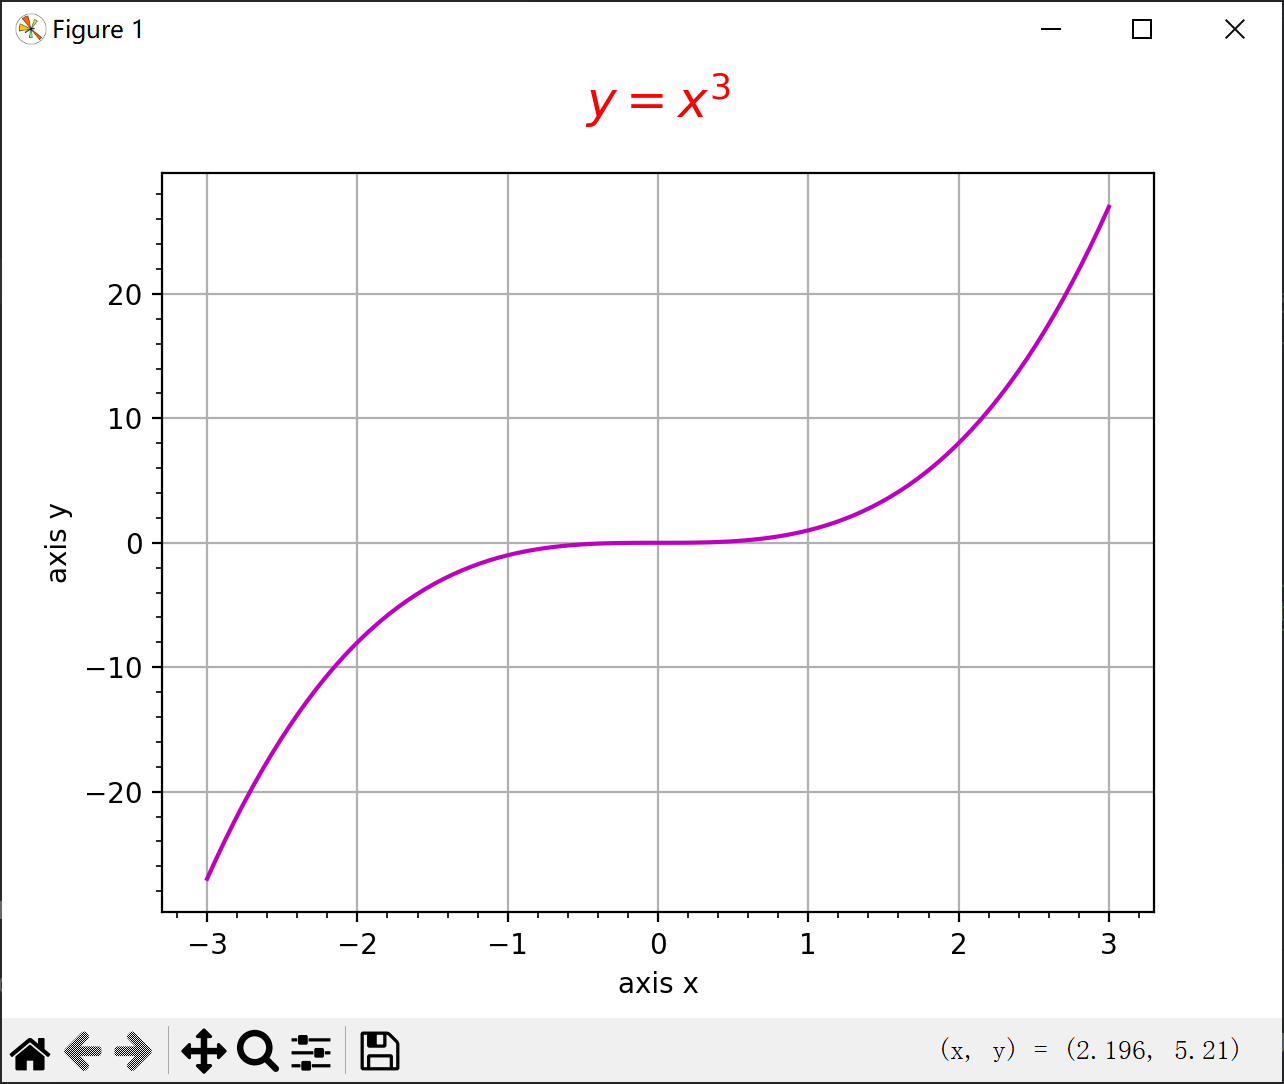
\includegraphics[width=0.5\linewidth]{Axes控制坐标轴 Pic1.png}
    \caption{4.3.2.1}
    \label{fig:enter-label}
\end{figure}

\subsubsection{再谈网格线grid}
我们知道,网格线是基于坐标轴上的刻度的,那么如何让添加的较小刻度也形成网格线呢?这就涉及到之前没有说的grid函数的更多设置。其主要设置如下:

\textit{\large grid(True, which=' ', axis=' ')}

其中which的可选值有major,minor和both,major代表仅主要刻度形成网格线,minor表示仅添加的较小刻度形成网格线,both表示所有刻度均形成网格线。

axis的可选值包括x,y和both。x表示仅x轴刻度形成网格线,即栅栏形(?),y同理,而both就是默认的状态,x,y均形成网格线。
举个例子,grid(True, which='both', axis='x')的效果如下图:
\begin{figure}[H]
    \centering
    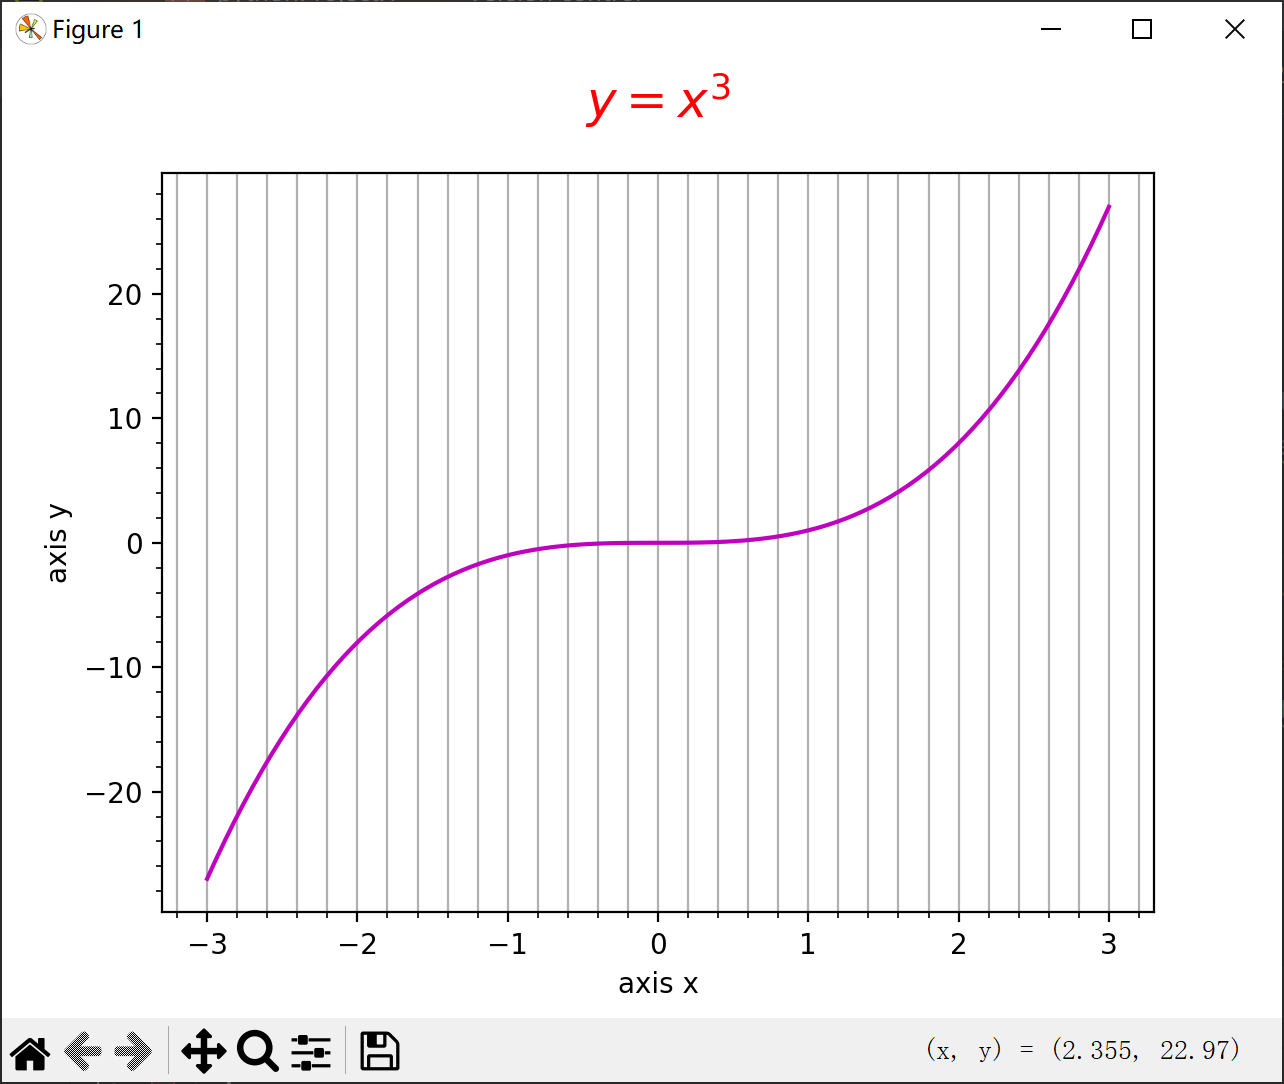
\includegraphics[width=0.5\linewidth]{grid Pic1.png}
    \caption{4.3.3.1}
    \label{fig:enter-label}
\end{figure}
\subsubsection{操控四条边框}
当我们已经把四条边框赋值给ax,(比如通过ax = plt.gca())我们就可以通过ax.spines['top'/'bottom'/'right'/'left']指定其中的任何一条边框进行操作。'top', 'bottom', 'right', 'left' 分别指上下左右四条边框。

我们可以以此设定边框的颜色,通过set\_color,比如ax.spines['right'].set\_color('red')就是把右边框设为红色。还可以设置x,y轴相交的位置,通过set\_position, 比如ax.spines['bottom'].set\_position(('data',a))即可将交界点设为在y=a的位置,x轴同理。最后我们甚至还可以设置边框宽度,通过set\_linewidth()。(要注意的是Axes方法不能链式调用,就是说ax.spines[ ]后面只能跟一个命令,别的命令就得另起一段了)

(顺带一提:如果set\_color('None'),那么颜色就是透明,也就是让边框不显示。)

如果我们要一次改变四条边框的某个参数比如宽度,一一指定未免太过麻烦,我们可以使用这样一个循环:

\[for\; spine\; in\; ax\,.\,spines\,.\,values(\,):\]
\[spine\,.\,set\_linewidth(2)\]
ax.spines是一个字典,包含四条边框,而ax.spines.values()是一个能返回使用边框的函数,因此我们可以用它来遍历所有边框。

在默认情况下,下边框和左边框分别是x,y轴,如果我们要设置其他边框为坐标轴,比如令上边框为x轴,右边框为y轴,可以使用如下命令:
\[ax.xaxis.set\_ticks\_position('top')\]
\[ax.yaxis.set\_ticks\_position('right')\]
此外,x,y轴的交界处也是可以设置的,如果要让x轴位于y=a位置,也就是交界点为(0,a),可以使用如下命令:
\[ax.spines['bottom'].set\_position(('data',a))\]
看到这行命令的你可能会有诸多疑问,比如这个双括号是什么,'data'又是什么。首先,set\_position()函数接受一个元组作为输入,因此出现了这样的“双括号”;这个元组的第一个元素'data'是一个字符串参数,它指定了接下来以什么形式指定坐标轴的位置,这个位置可以接受的字符串参数有:(以下统一称边框为“脊柱”)

1.   'outward'  :将脊柱向外移动一定的距离。默认情况下,距离为0,即脊柱紧贴坐标轴。 例如ax.spines['right'].set\_position(('outward', 10)) 表示将右侧脊柱向外移动10个单位。可以通过设置   set\_smart\_bounds   方法来调整距离。

2.   'axes'  :将脊柱的位置设置为坐标轴的相对位置,取值范围为0到1。例如,  ('axes', 0.5)   表示脊柱位于坐标轴的中间。

3.   'data'  :将脊柱的位置设置为数据坐标系中的某个位置。例如,  ('data', 3)   表示脊柱位于数据坐标系中的 x=3 或 y=3 处,如果指定的脊柱是左脊柱或右脊柱,则是x=3,反之则是y=3。

个人认为在大多数时候,‘data’法是最好用的,因此接下来重点介绍它。

讲到这里,必须要澄清一个很容易误会的点,Python在将子图绘制出来的时候,代表x,y的两脊柱相交在(0,0)处,但我们并不能说默认两脊柱相交在原点处,事实上,在你人为设定交点前,不存在任何脊柱的交点,如果你点击下方十字箭头标志,然后拖动图像,你会发现交界点固定在原地,不会随原点移动,但是如果我们增加这样一个交界点的设置,情况就正好相反,我们用如下程序进行演示:
\begin{figure}[H]
    \centering
    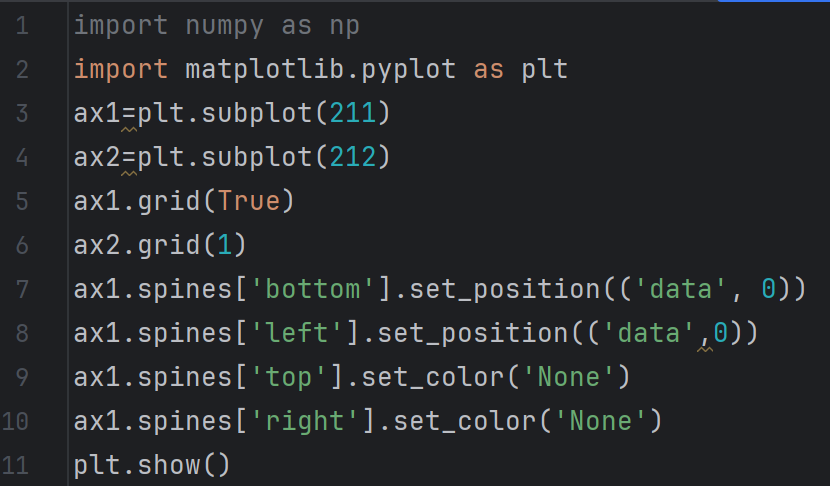
\includegraphics[width=0.6\linewidth]{脊柱设置 program1.png}
    \caption{4.3.4.1}
    \label{fig:enter-label}
\end{figure}

\begin{figure}[H]
    \centering
    \begin{subfigure}[b]{0.45\textwidth}
        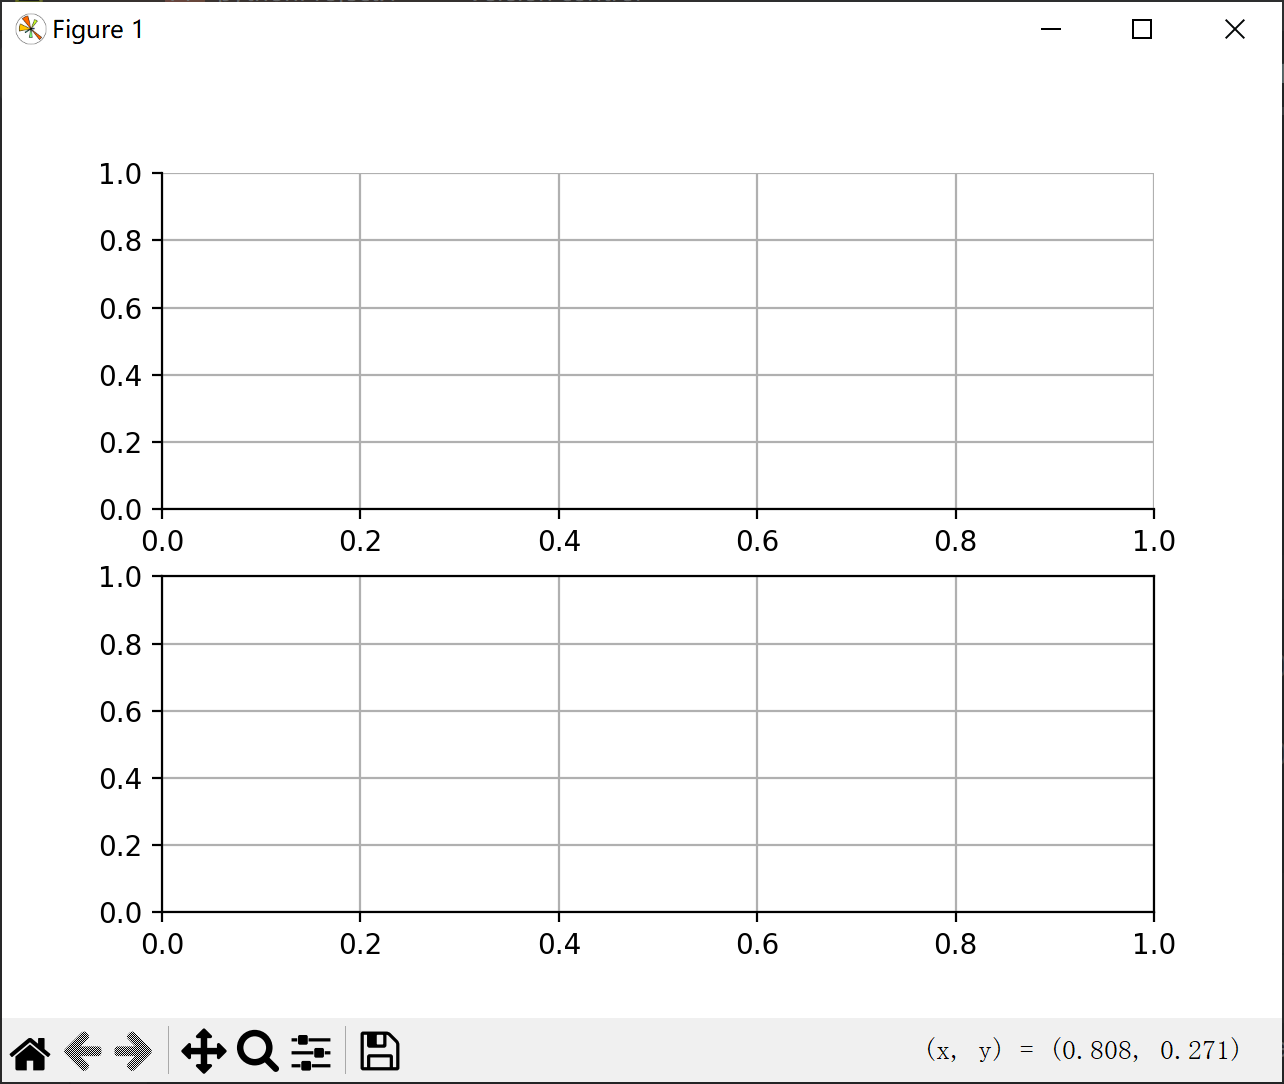
\includegraphics[width=\textwidth]{脊柱设置 Pic1.png} % 确保图片宽度不超过页面宽度
        \caption{4.3.4.2 拖动前}
        \label{fig:line-graph2}
    \end{subfigure}
    \hfill
    \begin{subfigure}[b]{0.45\textwidth}
        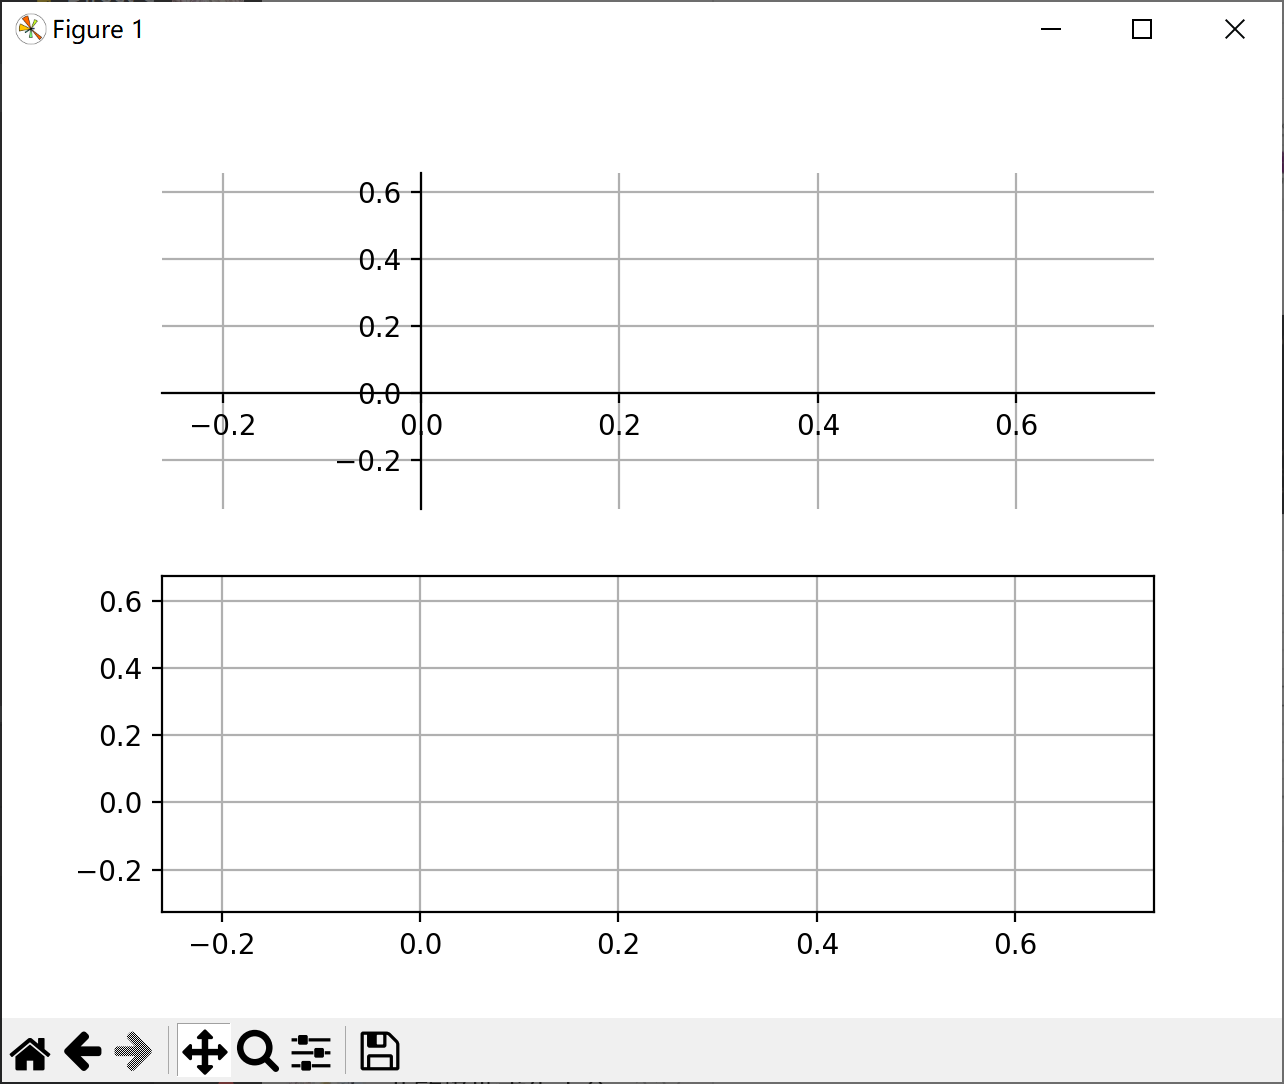
\includegraphics[width=\textwidth]{脊柱设置 Pic2.png} % 确保图片宽度不超过页面宽度
        \caption{4.3.4.3 拖动后}
        \label{fig:line-graph2-pic2}
    \end{subfigure}
\end{figure}


\subsubsection{其他}
还有一些零碎的,没那么重要的设置,这里简单提一下:

\noindent \textbf{\large 设置轴矩形补丁:}

set\_frame\_on(True/False)设置是否绘制轴矩形补丁,默认是True。这个轴矩形补丁其实就是边框,如果为False,四条边框就会被隐藏。

\noindent \textbf{\large 设置轴刻度线和网格线位置:}

set\_axisbelow(True/False) 设置轴刻度线和网格线是在图上方还是下方,True 则将刻度线和网格线设置在图下方,反之则在上方。
\newpage
\section{极坐标系}
\subsection{极坐标系简介}
\begin{figure}[H]
    \centering
    \includegraphics[width=0.75\linewidth]{极坐标 program1.png}
    \caption{5.1.1.1}
    \label{fig:enter-label}
\end{figure}
极坐标系的函数是plt.polar(),与plot函数相似,polar先接受两个确定二维平面内点位置的数据,然后接受其他参数的设置,我们知道,在极坐标系中,确定位置的两个量是角度和距离,我们通常设定为theta和r。然后,类似在直角坐标系中的做法,我们利用np.linspace对自变量theta进行指定区间内的大量取点,在示例中就是取满0~360度,然后列出r关于theta的关系式就可以了,是不是跟直角坐标系中的plot函数非常相似呢?\textcolor{red}{(要注意的是传递给polar函数时是角度在前,距离在后,这也不难理解,因为角度是自变量嘛)}

上面这段代码绘制出的,就是著名的“笛卡尔心形线”了,效果如下:
\begin{figure}[H]
    \centering
    \includegraphics[width=0.5\linewidth]{极坐标 Pic1.png}
    \caption{5.1.1.2}
    \label{fig:enter-label}
\end{figure}
就这张图,讲讲极坐标系图的几个基本概念。周围一圈角度值叫角度刻度,内部一环环上标的数值叫半径刻度(我有时候喜欢称之为“圆周刻度”),你会发现,极坐标系的角度和半径可以分别对应直角坐标系的x和y轴,事实上,matplotlib也是这样设定的,后面会讲到的用于设置极坐标系刻度的函数分别是set\_xticklabels(),set\_yticklabels(),这就是把xticklabels视为角度刻度,把yticklabels视为半径刻度。
\subsection{极坐标系的复杂设置}
\noindent 下面介绍polar函数一些更复杂的设置:

\noindent \textbf{标记点样式相关参数:}

1. marker:标记点样式,如   'o'   表示圆形标记点,  '*'   表示星号标记点等。

2. markersize(ms):标记点的大小,数值越大,标记点越大。

3. markerfacecolor(mfc):标记点的填充颜色,可以是颜色名称字符串(如   'red'  )、十六进制颜色代码(如   '\#FF0000'  )等。

4.markeredgecolor(mec):标记点的边界颜色,设置方法与   markerfacecolor   类似。

\noindent \textbf{线条样式相关参数:}

老生常谈的color,linestyle,linewidth(lw),label和alpha。

\noindent \textbf{坐标轴相关:}

极坐标系的坐标轴方法有一些和直角坐标系是相同的,比如创建子图的方法;还有plt.grid()(或者ax.grid())可以用Ture,False控制网格的有无,唯一的区别是在极坐标系中,网格是默认为“有”的;最后plt.title()依然可以添加标题或其他文字。

其他的方法则稍有区别,比如在直角坐标系中设置坐标轴刻度范围和位置的函数是xticks和yticks,在极坐标系中则是set\_thetagrids()设置角度,set\_rgrids()设置半径(注意这俩是Axes方法啊!不是plt),通常做法是向它们传递一个确定始末点和步长的numpy数组,然后再传递一个长度相同的列表labels=[ ]确定这些刻度的名称。

如果要改变所有刻度的某个参数或依次指定,该怎么办呢?以角度刻度和颜色参数为例,我们可以用get\_xticklabels函数获取所有的角度标签(刻度),赋值给一个变量:
\[labels\; =\; ax1.get\_xticklabels(\,)\]

然后利用zip,在一个循环中改变所有的角度刻度:
\[for\; label\,,\, color\; in\; zip(labels,\, colors):\]
    \[label.set_color(color)\qquad\]
colors是一个颜色列表,其长度一个等于labels长度,通过这两个列表元素的一一对应,我们实现了对每个刻度颜色的指定,当然如果我希望所有刻度但是一个颜色,我们可以无视对colors的遍历,直接指定set\_color中的color是什么颜色。如果color被指定为‘None’,那么所有刻度就被抹除了。

但是要注意的是虽然我无视了这个颜色列表,这个列表依然必须存在。如果希望彻底摆脱它,我们可以省去colors和zip函数,直接对labels遍历。

结合这些方法和我们前面所学的方法,我们可以在“笛卡尔心形线”基础上整出非常多的活:
\begin{figure}[H]
    \centering
    \includegraphics[width=0.65\linewidth]{极坐标 Pic2.png}
    \caption{5.2.1.1}
    \label{fig:enter-label}
\end{figure}
\begin{figure}[H]
    \centering
    \includegraphics[width=0.65\linewidth]{极坐标 Pic3.png}
    \caption{5.2.1.2}
    \label{fig:enter-label}
\end{figure}
\noindent 请读者思考一下如何实现这些效果。
\newpage
图5.2.1.1代码:
\begin{figure}[H]
    \centering
    \includegraphics[width=1\linewidth]{极坐标 program2.png}
    \caption{5.2.1.3}
    \label{fig:enter-label}
\end{figure}
这里需要解释一个之前没有提到的点,如果我们需要创建多子图,就必须要使用Axes方法进行绘图,因为我们需要指定各个ax绘制不同的图像。但是Axes方法并没有极坐标系函数,就是说没有ax.polar()这个东西。那么我们就需要用另一种方法建立极坐标系,在plt.subplot()中指定projection='polar'。这个projection参数我们在3D图绘制还会遇到它,有关它的详细介绍我们放在详述\ref{projection参数:投影类型的指定}。
\newpage
图5.2.1.2代码:
\begin{figure}[H]
    \centering
    \includegraphics[width=1\linewidth]{极坐标 program3 1.png}
    \caption{5.2.1.4}
    \label{fig:enter-label}
\end{figure}
\begin{figure}[H]
    \centering
    \includegraphics[width=1\linewidth]{极坐标 program3 2.png}
    \caption{5.2.1.4续}
    \label{fig:enter-label}
\end{figure}
(顺带一提,图5.2.1.2所示代码中的颜色元组是下一个section要说的RGB模式自定义颜色,其数值是本人试验了一个晚上,与各高校校徽颜色反复比对出来的最佳配比,只有HIT是依据个人喜好设定的。手动[doge])


\newpage
\section{3D图像}
\subsection{3D图总览}
3D图像,本质上就是比平面图多了一个变量,多了一个维度,根据matplotlib所能呈现出的效果,我们可以大致将3D图像分为3D 线图、3D 散点图、3D 曲面图、3D 线框图、3D 等高线图这几类。下面我们分别展示这几类图是什么效果:

\textbf{\Large 3D 线图}

\begin{figure}[H]
    \centering
    \begin{subfigure}[b]{0.48\textwidth}
        \includegraphics[width=\textwidth]{3D exap Pic1.png} % 确保图片宽度不超过页面宽度
        \caption{6.1.1.1}
        \label{fig:line-graph2}
    \end{subfigure}
    \hfill
    \begin{subfigure}[b]{0.48\textwidth}
        \includegraphics[width=\textwidth]{3D exap program1.png} % 确保图片宽度不超过页面宽度
        \caption{6.1.1.2}
        \label{fig:line-graph2-pic2}
    \end{subfigure}
\end{figure}

\textbf{\Large 3D 散点图}

\begin{figure}[H]
    \centering
    \begin{subfigure}[b]{0.48\textwidth}
        \includegraphics[width=\textwidth]{3D exap Pic2.png} % 确保图片宽度不超过页面宽度
        \caption{6.1.1.3}
        \label{fig:line-graph2}
    \end{subfigure}
    \hfill
    \begin{subfigure}[b]{0.48\textwidth}
        \includegraphics[width=\textwidth]{3D exap program2.png} % 确保图片宽度不超过页面宽度
        \caption{6.1.1.4}
        \label{fig:line-graph2-pic2}
    \end{subfigure}
\end{figure}
\newpage
\textbf{\Large 3D 曲面图}

\begin{figure}[H]
    \centering
    \begin{subfigure}[b]{0.48\textwidth}
        \includegraphics[width=\textwidth]{3D exap Pic3.png} % 确保图片宽度不超过页面宽度
        \caption{6.1.1.5}
        \label{fig:line-graph2}
    \end{subfigure}
    \hfill
    \begin{subfigure}[b]{0.48\textwidth}
        \includegraphics[width=\textwidth]{3D exap program3.png} % 确保图片宽度不超过页面宽度
        \caption{6.1.1.6}
        \label{fig:line-graph2-pic2}
    \end{subfigure}
\end{figure}

\textbf{\Large 3D 线框图}

\begin{figure}[H]
    \centering
    \begin{subfigure}[b]{0.48\textwidth}
        \includegraphics[width=\textwidth]{3D exap Pic4.png} % 确保图片宽度不超过页面宽度
        \caption{6.1.1.7}
        \label{fig:line-graph2}
    \end{subfigure}
    \hfill
    \begin{subfigure}[b]{0.48\textwidth}
        \includegraphics[width=\textwidth]{3D exap program4.png} % 确保图片宽度不超过页面宽度
        \caption{6.1.1.8}
        \label{fig:line-graph2-pic2}
    \end{subfigure}
\end{figure}
\newpage
\textbf{\Large 3D 等高线图}

\begin{figure}[H]
    \centering
    \begin{subfigure}[b]{0.48\textwidth}
        \includegraphics[width=\textwidth]{3D exap Pic5.png} % 确保图片宽度不超过页面宽度
        \caption{6.1.1.9}
        \label{fig:line-graph2}
    \end{subfigure}
    \hfill
    \begin{subfigure}[b]{0.48\textwidth}
        \includegraphics[width=\textwidth]{3D exap program5.png} % 确保图片宽度不超过页面宽度
        \caption{6.1.1.10}
        \label{fig:line-graph2-pic2}
    \end{subfigure}
\end{figure}

\subsection{浅析3D图}

\subsubsection{3D空间的创建}
要绘制 3D 图像,首先需要创建一个 3D 绘图区域,即   Axes3D   对象,同创建极坐标系的方法一样,在plt.subplot或fig.add\_subplot函数中令projection=‘3d’,有三件事要注意:一是有些版本的matplotlib支持在gca函数中令projection=‘3d’,有些则不支持,个人建议是尽量别用这个方法了;二是我们令projection=‘3d’时其实是在使用   Axes3D   类,在比较高版本Matplotlib里,  Axes3D   已经被集成到 Matplotlib 的核心模块中,因此不需要显式导入它,否则需要在开头进行导入:
\[from\;\; mpl\_toolkits\,.\,mplot3d\;\; import\;\; Axes3D\] 
三是注意projection=‘3d’中,‘d’是小写!!

与极坐标系图不同,3D图像不存在可以代替设置projection的pyplot方法,对于那些专门绘制特殊3D图像如曲面图、等高线图的方法,它们只能在projection=‘3d’的情况下被使用,否则会直接报错。

\subsubsection{3D图像再划分——何时要meshgrid}
我们先简单回忆一下平面图像是如何作出来的,首先通过x=np.linspace(),x大量取点,一一映射到y,从而确定平面上每一个点的坐标,现在对于三维坐标系,自变量可以是一个,也可以是两个,这两种情况实际上很大程度上决定了后面可以用哪些3D方法以及要不要使用meshgrid。

变量只有一个的比较简单,比如z是自变量,x和y都是它的因变量,这相当于将平面直角坐标系的因变量轴拆出了两个轴,但是它们依然都是受z控制的。下面是一个单变量的例子:
\begin{figure}[H]
    \centering
    \includegraphics[width=0.5\linewidth]{3D mesh program1.png}
    \caption{6.2.2.1}
    \label{fig:enter-label}
\end{figure}
因为我们分别用z计算(定义)了x和y,z的定义是一个一维numpy数组,因此x和y也是一维数组,类型相同,我们就可以把它们一起丢进plot进行作图了。最终效果如下,可见垂直z轴任何一个平面截图像,永远只能截出一个点。
\begin{figure}[H]
    \centering
    \includegraphics[width=0.5\linewidth]{3D mesh Pic1.png}
    \caption{6.2.2.2}
    \label{fig:enter-label}
\end{figure}
如果变量有两个,比如令x=np.linspace(a,b,n),y=np.linspace(c,d,m),z=f(x,y),此时我们就不能贸然直接计算z了。因为我们说x,y两个变量时,我们希望的是x,y这个平面作为自变量,平面上的每个点对应一个z值,但是两个数组直接运算时,如果它们长度不同,即m!=n,那么程序会直接报错,因为长度不同的两个数组是不能直接运算的;如果它们长度相同,即m=n,那么元素会一一对应进行运算,最后生成一个由每一对元素计算结果组成的,长度一样的新一维数组,这显然不是我们想要的,呃,或者说大多数时候不会是我们想要的。

下面这个例子可以很好地展现长度相同的x,y直接运算得到z会发生什么:
\begin{figure}[H]
    \centering
    \includegraphics[width=0.65\linewidth]{3D mesh program2.png}
    \caption{6.2.2.3}
    \label{fig:enter-label}
\end{figure}
\begin{figure}[H]
    \centering
    \begin{subfigure}[b]{0.4\textwidth}
        \includegraphics[width=\textwidth]{3D mesh Pic2.1.png} % 确保图片宽度不超过页面宽度
        \caption{6.2.2.4 未正对状态}
        \label{fig:line-graph2}
    \end{subfigure}
    \hfill
    \begin{subfigure}[b]{0.4\textwidth}
        \includegraphics[width=\textwidth]{3D mesh Pic2.2.png} % 确保图片宽度不超过页面宽度
        \caption{6.2.2.5 z轴正对状态}
        \label{fig:line-graph2-pic2}
    \end{subfigure}
\end{figure}
但是如果我们在z1=x**2-y**2前加上x, y = np.meshgrid(x, y),图像就会变成如下这样:
\begin{figure}[H]
    \centering
    \includegraphics[width=0.5\linewidth]{3D mesh Pic2.3.png}
    \caption{6.2.2.5}
    \label{fig:enter-label}
\end{figure}
可以看到已经很接近我们心目中3D图的样子了对吧,meshgrid的作用就是生成二维网格,或者更确切的说,x, y = np.meshgrid(x, y)是将x, y这两个\textcolor{red}{长度可以不同}的一维数组变成两个可以运算的二维数组(两个可以运算的矩阵)具体做法是在另一个方向上复制自己至对方的长度(???)没关系,我们来看一个例子:
\begin{figure}[H]
    \centering
    \includegraphics[width=1\linewidth]{3D mesh Pic3.png}
    \caption{6.2.2.6}
    \label{fig:enter-label}
\end{figure}
它的代码放在后面,在左边我分别令x, y是0~5六个整数组成的列表,然后对它们用meshgrid,最后分别打印出x, y,可以看到它们分别在对方的方向上把自己(0,1,2,3,4,5)复制了6次,如此一来二者就可以形成一张二维网格,可以进行运算。对照右边的网格图,我专门调整了x,y轴位置和刻度位置,可以很清楚的看出x打印出来就是所有横坐标的矩阵,y打印出来就是所有纵坐标的矩阵。至于为什么meshgrid被设计的将x,y在不同的方向复制,这是否与矩阵的运算有关,请读者自行思考。

总之,如果我们希望两个自变量组成的平面能够作为自变量,即形成网格,就需要在运算前对它们使用meshgrid,将它们转换为可以运算的二维数组,这样因变量的也会成为一个二维数组,它们就可以用来生成图像了。

一个小提醒,在两个自变量取点数一样多的情况下,线图(plot)和点图(scatter)都是不会报错的,但是曲面图,网格图,等高线图仍然会报错,它们的绘制必须提前使用meshgrid方法。
\begin{figure}[H]
    \centering
    \includegraphics[width=0.75\linewidth]{3D mesh program3.png}
    \caption{6.2.2.7}
    \label{fig:enter-label}
\end{figure}

\subsection{各类3D图的方法}
\subsubsection{线图与点图}

这一节我们开始详细介绍各种3D图绘制的方法。首先是线图和点图,3D图的线图,点图与平面图其实差异不大,平面图中的那些设置在3D图中基本一样适用。最本质的区别还是多了一个维度,要向plot或scatter传递的参数多了一个。至于x,y,z是否需要在建立关系的时候使用meshgrid构建网格,完全依照实际需求。很有意思的是,如果我们让x,y=np.meshgrid(x,y),x,y变成了两个二维数组,而z还是一维数组,这时把它们丢进scatter或plot并不会出现报错,这时因为numpy数组自带一套广播机制,维度小的数组会通过在一个方向上复制自身来匹配其它数组的维度,具体请参考这里\ref{广播机制}。

\subsubsection{曲面图}
曲面图基本语法如下:
\[ax\,.\,plot\_surface(x,y,z,**kwargs)\]
其中x,y,z,都是二维数组,通常是x,y由meshgrid   函数生成,z由x,y计算得到。**kwargs指其它设置的参数,其中包括我们早就熟悉的透明度alpha,颜色映射cmap,还有线宽linewidth/lw,透明度和颜色映射都没什么好说的,忘了颜色映射的话click here:\ref{颜色映射}。线宽在这里出现可能会让你觉得很奇怪,这里线宽其实是曲面表面网格线的宽度,如果令其为0,则不显示网格线。(但是在我这个版本的matplotlib中3D曲面图网格线被整得很奇怪,它的出现与否并不受lw是否为0控制,而是受另一个参数抗锯齿antialiased是否=True控制,antialiased=True则由网格线,反之没有,而默认情况下就是antialiased=True,所以如果这两个参数你都不动,是会有网格线的;同时我们也知道了如果想要去掉网格线,只需要令antialiased=False就行了。

曲面上的网格线长这样:
\begin{figure}[H]
    \centering
    \includegraphics[width=0.75\linewidth]{3D 曲面图 网格线 Pic1.png}
    \caption{6.3.2.1}
    \label{fig:enter-label}
\end{figure}

其它一些参数包括抗锯齿antialiased,行和列的采样点数rcount  和  ccount 和阴影shade。

1. antialiased:我真的不想讲这个参数,在我目前看来它除了刚刚说的控制网格线的生成,没有任何用处,理论上它=True时能够使图形边缘更加平滑,反之图形边缘可能显得锯齿状,但可以提高渲染速度,适合需要快速绘制的场景,但我个人觉得效果很不明显。 它默认下是True。

2. rcount 和 ccount: rcount用于指定沿行方向的采样点数。ccount则用于指定沿列方向的采样点数,你可能会说,采点数难道不是我们在用np.linspace方法调用x,y时就确定了的吗,这其实是一个挺复杂的问题。\textcolor{red}{我们在一开始用np.linspace方法
去的点是原始数据,而最后真正的绘制(专业一点叫渲染)是从原始数据中抽取一部分来进行绘制}。比如说,我对x,y的定义是np.linspace(-5, 5, 100),那么它们在meshgrid 后会形成一个100*100的网格,共10000个数据点,但是如果令rcount=50,ccount=50,意味着最后是从100行中抽取50行,100列中抽取50列参与渲染,也就是只有2500个点。\textcolor{red}{总之,rcount 和 ccount的取值一定是小于linspace中的设定的,它们的作用是限制原始数据量,减少渲染时的计算量,避免因为数据量过大而导致绘图缓慢或内存不足,但同时图像精度也会降低。}因此,为了在高精度和渲染速度之间找到平衡,建议的做法是增大linspace的取点数,即抬高精度上限,然后调整rcount 和 ccount值找到最优位置。(旧版本的matplotlib有两个参数rstride和cstride,控制网格线的密度,但在新版本中已被基本废弃,被rcount 和 ccount取代。)

默认情况下rcount=50,ccount=50.

3. shade: 说来它的功能有点好笑,它用于控制是否为表面添加阴影效果,取值为布尔值。因为阴影效果可以使表面的立体感更强(?maybe)。shade=True时有阴影,反之没有。默认情况是True。

有意思的是,曲面为单一颜色时阴影有无很明显,但是采用颜色映射cmap时则几乎没有区别。
\begin{figure}[H]
    \centering
    \begin{subfigure}[b]{0.4\textwidth}
        \includegraphics[width=\textwidth]{3D 曲面图 shade Pic1.png} % 确保图片宽度不超过页面宽度
        \caption{6.3.2.2 shade=True}
        \label{fig:line-graph2}
    \end{subfigure}
    \hfill
    \begin{subfigure}[b]{0.4\textwidth}
        \includegraphics[width=\textwidth]{3D 曲面图 shade Pic2.png} % 确保图片宽度不超过页面宽度
        \caption{6.3.2.3 shade=False}
        \label{fig:line-graph2-pic2}
    \end{subfigure}
\end{figure}
\newpage
\subsubsection{线框图}
线框图的函数是plot\_wireframe,方法如下,其实跟曲面图一模一样,就是设置上略有不同:
\[ax\,.\,plot\_wireframe(x,y,z,**kwargs)\]
线框图函数的设置也有经典的颜色、透明度、线宽,不过这里的线宽就是线框的线宽,既然其主体是线条,自然少不了线框的样式linestyle,跟之前说过的一模一样,  '-'  (实线)、  '--'  (虚线)、  ':'  (点线)等。还有线框图也有 rcount 和 ccount,跟曲面图是一样的。

因为与曲面图相似度很高,到这里我们已经将线框图介绍完了,下面展示一个简单的线框图代码示例:
\begin{figure}[H]
    \centering
    \includegraphics[width=0.75\linewidth]{3D 线框图 program1.png}
    \caption{6.3.3.1}
    \label{fig:enter-label}
\end{figure}
\begin{figure}[H]
    \centering
    \includegraphics[width=0.5\linewidth]{3D 线框图 Pic1.png}
    \caption{6.3.3.2}
    \label{fig:enter-label}
\end{figure}
\newpage
\subsubsection{等高线图}
等高线图其实是一种平面图,我们一般并不会像第一部分所举的例子那样吧等高线图画仅空间坐标系的一个平面里,之所以把它放在这里说,是因为首先等高线图反映的其实是3D图,它相当于是将一幅3D图拍扁了,用二向箔降维打击了(?),其次它的方法与3D图非常相似,它的绘制也需要传递x,y,z三个参数,所以我们可以将其视为一种特殊的3D图。

我们首先看一个例子,上图:

\begin{figure}[H]
    \centering
    \includegraphics[width=1\linewidth]{3D 等高线图 Pic1.png}
    \caption{6.3.4.1}
    \label{fig:enter-label}
\end{figure}
\begin{figure}[H]
    \centering
    \includegraphics[width=0.8\linewidth]{3D 等高线图 program1.png}
    \caption{6.3.4.2}
    \label{fig:enter-label}
\end{figure}
% (且不说这种数据呈现方式有什么用,就说帅不帅?! 手动[doge])
\newpage
为了展示等高线图与它的祖宗3D曲面图的紧密关联,我在上面这个例子中将其相应的3D图一并绘制出来以作对照。整段代码中真正有关等高线图方法的只有下面这两行:
\[contours = ax1\,.\,contour(X,\,Y,\, Z,\;  levels=10,\, cmap=cmap,\, linewidths=1.5,\, linestyles='solid\,'\;)\]
\[ax1\,.\,clabel(contours,\, inline=True,\, fmt='\%1.1f\,',\, fontsize=10\;)\]
\noindent\textbf{X,Y,Z: }在等高线图中,原本的z轴值成为高度数据,以标签的形式显示出来,其传递方式还是和3D图的那些方法一样,x,y,z占据前三个参数。

\noindent\textbf{ levels:}指定等高线的数量或具体值。如果是整数   n  ,则会自动生成   n+1   个等高线级别,这些级别是等距的;如果是数组,则直接使用数组中的值作为等高线级别。

\noindent\textbf{linestyles和linewidths: }可以接受单个浮点数或字符串,也可以接受一个数组或列表,从而为每一条等高线设置不同的线形和线宽。

\noindent\textbf{fontsize: }就是高度标签的字体大小。

\noindent\textbf{inline:}布尔值,True的时候标签被嵌入等高线中,就是等高线会在标签处中断,反之等高线直接穿过标签(我想没人会喜欢这样吧)。默认是True,所以我觉得这个参数基本是不用动的。

\noindent\textbf{fmt:}格式化字符串,用于指定标签的格式,比如保留几位小数。详见\ref{格式化字符串表示保留小数位}

还有一些更复杂的设置,包括抗锯齿antialiased,locator,origin,extent等但是很多时候效果并不显著,而且比较繁复这里就不再介绍。
\newpage
\section{事件处理与交互}
在之前的章节中,我们都是写好一段代码,然后一键运行,它会生成一张相应的图像,但如果我希望在图像生成出来后直接对其进行一些操作呢?这就是我们本章要讨论的内容——事件的交互与处理。友情提示,本章内容难度可能会有一点点大哦。
\subsection{什么是事件处理与交互——事件机制概述}
为了帮助读者尽快熟悉这个陌生的概念,我们先来看一个简单的事件交互的例子:

\begin{figure}[H]
    \centering
    \begin{subfigure}[b]{0.45\textwidth}
        \includegraphics[width=\textwidth]{交互 Pic1.png} % 确保图片宽度不超过页面宽度
        \caption{7.1.1.1}
        \label{fig:line-graph2}
    \end{subfigure}
    \hfill
    \begin{subfigure}[b]{0.45\textwidth}
        \includegraphics[width=\textwidth]{交互 Pic1.2.png} % 确保图片宽度不超过页面宽度
        \caption{7.1.1.2}
        \label{fig:line-graph2-pic2}
    \end{subfigure}
\end{figure}
注意看,图7.1.1.1是一张平平无奇的直线线图,解析式是x-y=0,定义域在[0,1],但是如果我们用鼠标在上面点几下,会发现点过的地方出现了红点,同时该点坐标被打印了出来,如图7.1.1.2所示。

在这个例子中,我通过鼠标的点击使图像发生了变化,或者更确切的说,让整个程序的运行都发生了改变,因为被点击点的坐标也被打印出来了。外界的这些操作比如鼠标点击,被称作”事件“,这些事件对程序造成影响的过程就叫做事件的交互。

接下来我们来看看这个事件交互是如何实现的,以上示例的程序如图7.1.1.3:
\begin{figure}[H]
    \centering
    \includegraphics[width=0.55\linewidth]{交互 program1.png}
    \caption{7.1.1.3}
    \label{fig:enter-label}
\end{figure}
我们来分析一下这段程序:首先我们定义了一个函数onclick,它接受event事件对象,这个event包含所有可能的事件,然后我们通过event.xdata,event.ydata获取了事件发生位置的坐标,也就是鼠标点击的坐标,然后将它们打印出来以及绘制成红点,fig.canvas.draw()表示更新画布,从而让绘制的点立刻显示出来。以上就是函数onclick的全部功能。

7、8两行我们很熟悉了,就是创建了图形对象与子图,并在子图上绘制了一条直线。然后就是一行奇怪的命令:
\[cid\, = \,fig\,.\,canvas\,.\,mpl\_connect(\,'\,button\_press\_event\,\,'\;,\, onclick\,)\]
这个mpl\_connect是一个监听函数,它能将具体事件与函数连接在一起,比如在上例中,当它监听到button\_press\_event这个事件时,它就会调用onclick函数,从而实现了由事件触发函数。

通过上面这个例子,我们已经初步了解了matplotlib事件交互与处理的基本逻辑,总结一下,就是首先定义某个事件发生时所调用的函数,这个函数以事件对象event为参数,这样我们就能再函数里获取event的属性的数据了,像事件的坐标xdata,ydata就是一种属性。通过事件的属性数据我们可以定义对图像进行哪些操作,这就是一个事件触发函数。最后,我们通过mpl\_connect将具体事件与相应的触发函数连接起来,这样在特定事件被监听到时,对应的函数就会被执行。

matplotlib支持多种事件对象event,如下表:
\begin{table}[H]
    \centering
    \begin{tabular}{ll}
        \toprule
        \textbf{事件类型} & \textbf{触发情况} \\
        \midrule
        \texttt{button\_press\_event} & 鼠标按下 \\
        \texttt{button\_release\_event} & 鼠标释放 \\
        \texttt{motion\_notify\_event} & 鼠标移动 \\
        \texttt{scroll\_event} & 滚轮滚动 \\
        \texttt{key\_press\_event} & 按键按下 \\
        \texttt{key\_release\_event} & 按键释放 \\
        \texttt{pick\_event} & 拾取对象 \\
        \texttt{resize\_event} & 窗口大小改变 \\
        \texttt{close\_event} & 关闭窗口 \\
        \bottomrule
    \end{tabular}
    \caption{Matplotlib 事件类型一览表}
    \label{tab:matplotlib_events}
\end{table}

事件对象的属性就比较复杂了具体可参考表2,注意区分event.x和event.xdata,前者是像素坐标,后者才是我们广义的坐标系的坐标。



\begin{table}[H]
    \centering
    \begin{tabular}{ll}
        \toprule
        \textbf{属性} & \textbf{说明} \\
        \midrule
        \texttt{name} & 事件名称(如 \texttt{'button\_press\_event'}) \\
        \texttt{canvas} & 触发事件的 \texttt{FigureCanvas} 对象 \\
        \texttt{guiEvent} & 底层 GUI 事件(可能为 \texttt{None}) \\
        \texttt{inaxes} & 事件发生时鼠标所在的 \texttt{Axes}(否则 \texttt{None}) \\
        \texttt{x}, \texttt{y} & 事件发生时的像素坐标(窗口坐标系) \\
        \midrule
        \multicolumn{2}{c}{\textbf{鼠标事件(\texttt{MouseEvent})}} \\
        \midrule
        \texttt{xdata}, \texttt{ydata} & 数据坐标系中的 x/y(鼠标在 \texttt{Axes} 内时) \\
        \texttt{button} & 按钮编号(1=左键, 2=中键, 3=右键, 'up'/'down' 滚轮) \\
        \texttt{step} & 滚轮滚动步长(仅 \texttt{scroll\_event}) \\
        \texttt{dblclick} & 是否为双击事件(Matplotlib 3.4+) \\
        \midrule
        \multicolumn{2}{c}{\textbf{键盘事件(\texttt{KeyEvent})}} \\
        \midrule
        \texttt{key} & 按下的键(如 'a', 'ctrl', 'shift', 'left') \\
        \midrule
        \multicolumn{2}{c}{\textbf{拾取事件(\texttt{PickEvent})}} \\
        \midrule
        \texttt{mouseevent} & 关联的鼠标事件(\texttt{MouseEvent}) \\
        \texttt{artist} & 被拾取的 \texttt{Artist}(如 \texttt{Line2D}、\texttt{Patch}) \\
        \texttt{ind} & 若 \texttt{artist} 是 \texttt{Line2D} 或 \texttt{Collection},返回被拾取点的索引列表 \\
        \bottomrule
    \end{tabular}
    \caption{Matplotlib 事件对象 (\texttt{event}) 的属性}
    \label{tab:matplotlib_event_properties}
\end{table}

\subsection{一些需要阐明的和解释的}
\subsubsection{fig与canvas}
这两个概念比较容易混淆。之前说过,我们用fig=plt.figure()创建出来的是一个图形对象,它是 Matplotlib 中所有绘图元素的顶级容器,可以包含一个或多个子图,之前我们都是直接对它进行操作,从而创建和管理图形内容。

canvas是这些操作的底层实现,将fig管理的内容渲染到屏幕上或保存为文件,通常我们不需要直接操作它,因为它一直是自动处理的。而现在,由于它是图形与用户交互的界面,我们需要对这个画布进行直接操作。于是,这个本应是最显眼的概念(毕竟所有图像都是在canvas上渲染出来的嘛)到现在才正式进入我们的视野。

在级别上,figure是最高级容器,figure 对象包含一个 canvas 属性,canvas 是 figure 的绘图区域,负责实际的渲染工作。

\subsubsection{artist 艺术家?}
在 Matplotlib 中,  Artist   是一个非常通用的概念,几乎可以描述所有可以被绘制的图形对象。而在事件交互中,event.artist专指那些可以触发事件的对象。

 Artist是 Matplotlib 中的一个基类,几乎所有可以被绘制的图形对象都是   Artist   的子类。这些对象包括:
 
 1. 线条(  Line2D  ):用于绘制直线或曲线。 \textcolor{blue}{(通常是plot画出来的)}
 
 2. 散点(  PathCollection  ):用于绘制散点图。  \textcolor{blue}{(通常是scatter画出来的)}
 
 3. 矩形(  Rectangle  ):用于绘制矩形。  \textcolor{blue}{(plt.Rectangle函数画的,一个专门画矩形的函数)}
 
 4. 文本(  Text  ):用于添加文本注释。  \textcolor{blue}{(不用说了,text函数)}
 
 5. 图像(  AxesImage  ):用于显示图像。  \textcolor{blue}{(通常是imshow画出来的)}
 
 6. 坐标轴(  Axes  ):整个坐标轴区域。  
 
 7. 图形(  Figure  ):整个图形窗口。 

不难发现,最后两种Artist与前四种不一样,它们不是某一种几何图形,而是一种装图形的容器。于是,我们将Artist分为两类:原始艺术家(Primitive Artists)与容器艺术家(Container Artists),前四种称为原始艺术家,后两者是容器艺术家。容器艺术家是包含其他艺术家的对象,它们用于管理其内部的多个原始艺术家。

原始艺术家的访问很简单,它们通常由相应的绘图函数直接返回,比如一个Line2D的访问就是如line, = ax.plot(x, y, label="Line")。容器艺术家中子艺术家的访问则需要用到get\_children()函数,比如children = ax.get\_children()可以获得Axes中所有子艺术家。

get\_children()函数通常与区分艺术家类型的 isinstance()函数联合使用,这个函数的具体介绍放到详述\ref{isinstance()函数}

在事件交互中的event.artist在事件交互中,  event.artist   是触发事件的具体对象。只有那些可以触发事件的对象才会被赋值给   event.artist  。例如: 如果你点击了一个散点图中的某个点,  event.artist   是被点击的   PathCollection   对象。 如果你点击了一条线,  event.artist   是被点击的   Line2D   对象。 如果你点击了一个矩形, event.artist   是被点击的   Rectangle   对象。\ref{isinstance()函数}中的那个运用isinstance()函数的例子也是artist在事件交互中应用的很好的例子。

\subsection{事件交互的实战应用}
现在你已经掌握了事件交互与处理的基本概念,让我们在实际应用中加深对它的理解吧。

首先close\_event太简单了,一点意思也没有,这里就不讲它了。
\subsubsection{窗口大小改变}
下面我们来看看比较少见但也能整点活的resize\_event。这是在改变窗口大小时触发的事件,它的核心属性就是窗口的长宽。首先你必须要记住的是(虽然我其实经常记不住)默认状态下窗口长宽分别是640与480,最大值(全屏下)是1280与625。知道了这些我们就可以开整了[手动Doge],想想看如何让窗口与画布的颜色随着窗口的大小变化做相应的变化?(小提示,它们颜色的设置用set\_facecolor,但是这个函数不支持颜色映射哦)

本人写出的代码如下,仅供参考:
\begin{figure}[H]
    \centering
    \includegraphics[width=0.75\linewidth]{React resize program1.png}
    \caption{7.3.1.1}
    \label{fig:enter-label}
\end{figure}
我们来对它进行一番拉扯,看看效果如何:
\begin{figure}[H]
    \centering
    \begin{subfigure}[b]{0.6\textwidth}
        \includegraphics[width=\textwidth]{React resize Pic3.png} % 确保图片宽度不超过页面宽度
        \caption{7.3.1.2}
        \label{fig:line-graph2}
    \end{subfigure}
    \hfill
    \begin{subfigure}[b]{0.35\textwidth}
        \includegraphics[width=\textwidth]{React resize Pic4.png} % 确保图片宽度不超过页面宽度
        \caption{7.3.1.3}
        \label{fig:line-graph2-pic2}
    \end{subfigure}
\end{figure}

\begin{figure}[H]
    \centering
    \begin{subfigure}[b]{0.5\textwidth}
        \includegraphics[width=\textwidth]{React resize Pic1.png} % 确保图片宽度不超过页面宽度
        \caption{7.3.1.4}
        \label{fig:line-graph2}
    \end{subfigure}
    \hfill
    \begin{subfigure}[b]{0.15\textwidth}
        \includegraphics[width=\textwidth]{React resize Pic2.png} % 确保图片宽度不超过页面宽度
        \caption{7.3.1.5}
        \label{fig:line-graph2-pic2}
    \end{subfigure}
\end{figure}
由于不能使用cmap,我们只能通过RGB的方式设定变化的颜色,通过指数函数的使用,我们将长宽变化的幅度放大,同时又控制在0\~1之间。
\subsubsection{拖拽事件}
别急着划回55页的表格,那里面没有这个事件,它其实是鼠标点击事件与鼠标移动事件的结合产物。在以下这个例子中,我们会用之前提到的plt.Rectangle函数创建一个矩形,并让它变得可以拖动。
\begin{figure}[H]
    \centering
    \includegraphics[width=0.75\linewidth]{拖拽事件 program1.png}
    \caption{7.3.2.1}
    \label{fig:enter-label}
\end{figure}
\begin{figure}[H]
    \centering
    \includegraphics[width=0.75\linewidth]{拖拽事件 program2.png}
    \caption{7.3.2.2}
    \label{fig:enter-label}
\end{figure}

其效果如下,这个红色的矩形是可以拖动的。
\begin{figure}[H]
    \centering
    \includegraphics[width=0.5\linewidth]{拖拽事件 Pic1.png}
    \caption{7.3.2.3}
    \label{fig:enter-label}
\end{figure}

以上代码还有些地方要简单解释一下。rect.xy中,xy是矩形的一个属性,指矩形左下角的坐标。

contains是判断某要素是否在某区域内的函数,代码中用于判断鼠标点击是否发生在矩形内;你也许会好奇,这个attrd是啥,它在后面再也没有被用到,为什么把它之间删掉却会导致矩形不能拖动了。这就要说到Python的神奇语法规则,当几个变量直接等于一个拥有相同数量元素的元组时,Python会自动解包元组,将元素值一一赋给变量,比如这里就是,self.rect.contains(event)是一个两元素的元组。但是如果删去attrd,就变成了contains等于元组,因为一般的逗号占位在这种自动解包元组的情况下是不适用的,如果实在要占位需要用下划线:contains, \_ = self.rect.contains(event)。set\_x,set\_y函数没讲,但是它们的功能一看即知,这里就不多介绍了。

请读者自行思考,如何让矩形碰到边界就不能再被拖动了呢。
\subsubsection{鼠标、键盘、滚轮大杂烩}
结合之前所学的各种鼠标、键盘、滚轮事件,我们来制作一个绘画板,要求如下:

1. 具有typical,linear,circle三种模式;能绘制曲线、直线、圆三种几何图形。这三种模式可以通过键盘按动进行切换

2.在typical模式下,鼠标按住拖动时直接留下痕迹;在linear模式下,以鼠标按下位置为起点,松开位置为终点画出直线,且要求按住拖动时直线已经出现并另一头会跟着鼠标跑,同时直线旁标识出直线的长度;在circle模式下,拖动时所绘半径(是由圆心到圆周的画法)与圆周均已出现并随着鼠标动,半径的要求与直线一致。

3.已经绘制的在手动删除前必须保留在画布上,在按下delete键后清空整个画布。

4.画布在未手动调整显示范围时保持不动,不得自动改变范围。手动改变可以通过上下左右键挪动画布,也可以通过滚轮进行整体的缩放。

5.当前模式能够在画布上方显示出来。

本人所写代码如下:

\begin{lstlisting}[language=Python]
import matplotlib.pyplot as plt
import numpy as np

fig, ax = plt.subplots()
ax.set_xlim(-10, 10)
ax.set_ylim(-10, 10)
ax.set_aspect('equal')

class DrawState:
    def __init__(self):
        self.pressed = 0
        self.line_number = 0
        self.circle_number = 0
        self.x_list = []
        self.y_list = []
        self.lines = []
        self.radius_values = []
        self.exist_lines = []
        self.circles = []
        self.exist_circles = []
        self.figure_pattern = 'typical'
        self.x1, self.y1, self.x2, self.y2, self.r_value = None, None, None, None, None

state = DrawState()
ax.set_title(f"Current Mode: {state.figure_pattern}", color='blue')

def on_click(event):   #### 鼠标点击事件
    ax.scatter(event.xdata, event.ydata, color='r', s=10)
    plt.draw()
    state.pressed = 1 - state.pressed

def on_released(event):    #### 鼠标松开事件
    ax.scatter(event.xdata, event.ydata, color='r', s=10)
    plt.draw()
    state.pressed = 1 - state.pressed
    state.x_list = []
    state.y_list = []
    if state.figure_pattern == 'linear':
        state.line_number += 1
        state.exist_lines.append(state.lines[-1])
        if state.line_number >= 1:
            for line in state.exist_lines[-state.line_number:]:
                ax.add_line(line)
            fig.canvas.draw()
    if state.figure_pattern == 'circle':
        state.circle_number += 1
        state.exist_circles.append(state.circles[-1])
        if state.circle_number > 1:
            for circle in state.exist_circles[-state.circle_number:]:
                ax.add_line(circle)
            fig.canvas.draw()

def typical_move(event):       ###  一般曲线绘制函数
    if state.pressed == 1:
        state.x_list.append(event.xdata)
        state.y_list.append(event.ydata)
        ax.plot(state.x_list, state.y_list, c='r')
        plt.draw()

def linear_move(event):          ###   直线绘制函数
    if event.name == 'motion_notify_event' and state.pressed == 1 and event.inaxes is not None:
        state.x_list.append(event.xdata)
        state.y_list.append(event.ydata)
        state.x1 = state.x_list[0]
        state.y1 = state.y_list[0]
        state.x2 = state.x_list[-1]
        state.y2 = state.y_list[-1]
        if None in (state.x1, state.x2, state.y1, state.y2):
            raise ValueError("One or more coordinates are None. Please check the input data.")
        state.r_value = np.sqrt((state.x2 - state.x1) ** 2 + (state.y2 - state.y1) ** 2)
        line, = ax.plot([state.x1, state.x2], [state.y1, state.y2], c='r')
        state.lines.append(line)
        r = ax.text((state.x1 + state.x2) / 2 + 0.5, (state.y1 + state.y2) / 2 + 0.5, 'r={}'
                    .format(round(state.r_value, 2)),
                    fontdict={'fontsize': 10, 'fontweight': 'light', 'color': 'blue'})
        state.radius_values.append(r)
        if len(state.lines) > 1:
            for line in state.lines[:-1]:
                line.remove()
            state.lines = state.lines[-1:]
            plt.draw()

        if len(state.radius_values) > 1:
            for r in state.radius_values[:-1]:
                r.remove()
            state.radius_values = state.radius_values[-1:]
            plt.draw()
        plt.draw()
    return state.x1, state.x2, state.y1, state.y2, state.r_value

def circle_move(event):    ### 圆形绘制函数
    x1, x2, y1, y2, r_value = linear_move(event)
    theta = np.linspace(0, 2 * np.pi, 100)
    circle, = ax.plot(x1 + r_value * np.cos(theta), y1 + r_value * np.sin(theta), c='r')
    state.circles.append(circle)
    if len(state.circles) > 1:
        for circle in state.circles[:-1]:
            circle.remove()
        state.circles = state.circles[-1:]
        plt.draw()
    plt.draw()

def on_motion(event):        ####   整合各图形绘制的函数,鼠标移动控制
    if state.pressed == 1:
        if state.figure_pattern == 'typical':
            typical_move(event)
            plt.draw()
        if state.figure_pattern == 'linear':
            linear_move(event)
            plt.draw()
        if state.figure_pattern == 'circle':
            circle_move(event)
            plt.draw()

def pattern_change(event):   ### 键盘事件控制函数
    if event.name == 'key_press_event' and event.key == 'l':  ###直线
        state.figure_pattern = 'linear'
    elif event.name == 'key_press_event' and event.key == 'r':   ###圆
        state.figure_pattern = 'circle'
    elif event.name == 'key_press_event' and event.key == 't':   ###一般曲线
        state.figure_pattern = 'typical'
    if event.key == 'delete':   #### 清空 但是模式不变
        ax.clear()
        ax.set_xlim(-10, 10)
        ax.set_ylim(-10, 10)
        ax.set_aspect('equal')
        state.pressed = 0
        state.line_number = 0
        state.circle_number = 0
        state.x_list = []
        state.y_list = []
        state.lines = []
        state.radius_values = []
        state.exist_lines = []
        state.circles = []
        state.exist_circles = []
    if event.key == 'up':
        ax.set_ylim(ax.get_ylim()[0] + 0.1, ax.get_ylim()[1] + 0.1)
    if event.key == 'down':
        ax.set_ylim(ax.get_ylim()[0] - 0.1, ax.get_ylim()[1] - 0.1)
    if event.key == 'left':
        ax.set_xlim(ax.get_xlim()[0] - 0.1, ax.get_xlim()[1] - 0.1)
    if event.key == 'right':
        ax.set_xlim(ax.get_xlim()[0] + 0.1, ax.get_xlim()[1] + 0.1)
    fig.canvas.draw()
    ax.set_title(f"Current Mode: {state.figure_pattern}", color='blue')

def on_scroll(event):
    ax.set_xlim(ax.get_xlim()[0] * (1 - event.step * 0.01), ax.get_xlim()[1] * (1 - event.step * 0.01))
    ax.set_ylim(ax.get_ylim()[0] * (1 - event.step * 0.01), ax.get_ylim()[1] * (1 - event.step * 0.01))
    fig.canvas.draw()

fig.canvas.mpl_connect('button_press_event', on_click)
fig.canvas.mpl_connect('button_release_event', on_released)
fig.canvas.mpl_connect('motion_notify_event', on_motion)
fig.canvas.mpl_connect('key_press_event', pattern_change)
fig.canvas.mpl_connect('scroll_event', on_scroll)

plt.show()
\end{lstlisting}
PDF没法显示动图,所以这里只好放一张画完后的画布效果图。
\begin{figure}[H]
    \centering
    \includegraphics[width=0.65\linewidth]{React 大杂烩 Pic1.png}
    \caption{7.3.3.1}
    \label{fig:enter-label}
\end{figure}
其实这个程序还有一个早些版本,不用class,而且也没加上实时展示当前状态以及缩放画布等功能,如下展示。但是不用class就意味着大量使用global来定义全局变量,通常这种全局变量特别多的程序中,使用class是一个比较好的选择。
\begin{lstlisting}[language=Python]
import matplotlib.pyplot as plt
import numpy as np

fig, ax = plt.subplots()
pressed = 0
x_data = []
y_data = []
cir = 0
lin = 0
lines = []
radius = []
exist_radius = []
exist_lines = []
exist_linear=[]
circle_number = 0
line_number = 0

ax.set_xlim(-10, 10)
ax.set_ylim(-10, 10)
ax.set_aspect('equal')

def clickon(event):
    global pressed, x_data, y_data, cir
    if event.inaxes is not None and cir == 0:
        ax.scatter(event.xdata, event.ydata, c='m', s=10)
        pressed = 1
        plt.draw()
    if event.inaxes is not None and cir == 1:
        ax.scatter(event.xdata, event.ydata, c='m', s=10)
        ax.text(event.xdata + 0.5, event.ydata + 0.5, '({},{})'.format(round(event.xdata, 2), round(event.ydata, 2)), fontdict={'fontsize': 10, 'fontweight': 'light', 'color': 'blue'})
        pressed = 1
        plt.draw()

def release(event):
    global pressed, x_data, y_data, cir, circle_number, line_number, exist_radius, exist_lines,exist_linear
    if event.inaxes is not None and cir+lin == 0:
        ax.scatter(event.xdata, event.ydata, c='m', s=10)
        pressed = 0
        plt.draw()
        x_data = []
        y_data = []
    elif event.inaxes is not None and len(x_data) >= 2 and cir+lin == 1:
        x1, y1 = x_data[0], y_data[0]
        x2, y2 = x_data[-1], y_data[-1]
        r = np.sqrt((x1 - x2) ** 2 + (y1 - y2) ** 2)
        if cir==1:
            theta = np.linspace(0, 2 * np.pi, 100)
            x_circle = x1 + r * np.cos(theta)
            y_circle = y1 + r * np.sin(theta)
            ax.plot(x_circle, y_circle, c='m')  # 绘制圆
        line_number += 1
        exist_lines.append(lines[-1])
        exist_linear.append(r)
        if line_number >= 1:
            for line in exist_lines[-line_number:]:
                ax.add_line(line)
            fig.canvas.draw()
        plt.draw()
        x_data = []
        y_data = []
        pressed = 0
    elif len(x_data) < 2 or lin==1:
        ax.scatter(event.xdata, event.ydata, c='m')
        plt.draw()

def moving(event):
    global pressed, x_data, y_data, cir, lines, radius, exist_lines, exist_radius
    if event.name == 'motion_notify_event' and pressed == 1 and event.inaxes is not None and cir + lin == 0:
        x_data.append(event.xdata)
        y_data.append(event.ydata)
        ax.plot(x_data, y_data, c='m')
        plt.draw()
    if event.name == 'motion_notify_event' and pressed == 1 and event.inaxes is not None and cir + lin != 0:
        x_data.append(event.xdata)
        y_data.append(event.ydata)
        x1, y1 = x_data[0], y_data[0]
        x2, y2 = x_data[-1], y_data[-1]
        if cir==1:
            line, = ax.plot([x1, x2], [y1, y2], c='r')
        else:
            line, = ax.plot([x1, x2], [y1, y2], c='m')
        ra = np.sqrt((x1 - x2) ** 2 + (y1 - y2) ** 2)
        if cir == 1 and lin == 0:
            r = ax.text((x1 + x2) / 2 + 0.5, (y1 + y2) / 2 + 0.5, 'r={}'.format(round(ra, 2)), fontdict={'fontsize': 10, 'fontweight': 'light', 'color': 'blue'})
        if cir == 0 and lin == 1:
            r = ax.text((x1 + x2) / 2 + 0.5, (y1 + y2) / 2 + 0.5, 's={}'.format(round(ra, 2)), fontdict={'fontsize': 10, 'fontweight': 'light', 'color': 'blue'})
        lines.append(line)
        radius.append(r)
        plt.draw()
        if len(lines) > 1:
            for line in lines[:-1]:
                line.remove()
            lines = lines[-1:]  # 保留最后一个线条
            fig.canvas.draw()
        if len(radius) > 1:
            for r in radius[:-1]:
                r.remove()
            radius = radius[-1:]  # 保留最后一个文本
            fig.canvas.draw()

def circle(event):
    global cir, lin
    if event.key == 'r':
        cir = 1 - cir
        lin = 0

def linear(event):
    global lin, cir
    if event.key == 'l':
        lin = 1 - lin
        cir = 0

def clear_all(event):
    global pressed, x_data, y_data, cir, lines, radius, exist_lines, exist_radius, circle_number, line_number
    if event.key == 'delete':
        ax.clear()
        ax.set_xlim(-10, 10)
        ax.set_ylim(-10, 10)
        ax.set_aspect('equal')
        fig.canvas.draw()
        lines = []
        radius = []
        exist_radius = []
        exist_lines = []
        circle_number = 0
        line_number = 0

cid1 = fig.canvas.mpl_connect('button_press_event', clickon)
cid2 = fig.canvas.mpl_connect('button_release_event', release)
cid3 = fig.canvas.mpl_connect('motion_notify_event', moving)
cid4 = fig.canvas.mpl_connect('key_press_event', linear)
cid5 = fig.canvas.mpl_connect('key_press_event', circle)
cid6 = fig.canvas.mpl_connect('key_press_event', clear_all)

plt.show()

\end{lstlisting}
而且想必读者在认真思考后会发现,这个先前版本的代码逻辑没有新版那么清晰,新版的代码基本做到了每个事件定义一个函数,而不是多个函数指向同一个事件(这么干多了容易出问题)。

同时在实际操作时本人发现,由于窗口出现后输入总会自动跳为中文,输入字母控制模式时总是有不必要的干扰出现(你懂的),因此改为由shift键切换模式更为方便,毕竟只有三个模式可切换。修改pattern\_change函数的前面部分即可。修改后的pattern\_change函数如下:
\begin{lstlisting}[language=Python]
def pattern_change(event):   ### 键盘事件控制函数
    if event.name=='key_press_event' and event.key=='shift':  ###  由shift键操控
        state.shift_number+=1

    if state.shift_number%3==2:  ###直线
        state.figure_pattern='linear'
    elif state.shift_number%3==1:   ###圆
        state.figure_pattern='circle'
    elif state.shift_number%3==0:   ###一般曲线
        state.figure_pattern='typical'
    if event.key == 'delete':   #### 清空 但是模式不变
        ax.clear()
        ax.set_xlim(-10, 10)
        ax.set_ylim(-10, 10)
        ax.set_aspect('equal')
        state.pressed = 0
        state.line_number = 0
        state.circle_number = 0
        state.x_list = []
        state.y_list = []
        state.lines = []
        state.radius_values = []
        state.exist_lines = []
        state.circles = []
        state.exist_circles = []
    if event.key == 'up':
        ax.set_ylim(ax.get_ylim()[0] + 0.1, ax.get_ylim()[1] + 0.1)
    if event.key == 'down':
        ax.set_ylim(ax.get_ylim()[0] - 0.1, ax.get_ylim()[1] - 0.1)
    if event.key == 'left':
        ax.set_xlim(ax.get_xlim()[0] - 0.1, ax.get_xlim()[1] - 0.1)
    if event.key == 'right':
        ax.set_xlim(ax.get_xlim()[0] + 0.1, ax.get_xlim()[1] + 0.1)
    ax.set_title(f"Current Mode: {state.figure_pattern}", color='blue')
    fig.canvas.draw()
\end{lstlisting}
\subsubsection{拾取事件}
例子见\ref{isinstance()函数},这就是一个经典的拾取事件展示。

\newpage
%%%%%%%%%%%%%%%%%%%%%%%%%%%%%%%%%%%%%%%%%%%%%%%%%%%%%%%%%%%%%%%%%%%%%%%%%%%%%%%%%%%%%%%%%%%%%%%%%%%%%%%%%%%%%%%%%%%%%%%%%%%%%%%%%%%%%%%%%%%%%%%%%%%%%%%%%%%%%%%%%%%%%%%%%%%%%%%%%%%%%%%%%%%%%%%%%%%%%%%%%%%%%%%%%%%%%%%%%%%%%%%%%%%%%%%%%%

\section{详述}\label{详述}
\subsection{如何利用Python解方程}\label{如何利用Python解方程}
利用Python解方程的方法很多,包括使用SymPy,使用SciPy,牛顿法等等,这一部分我们主要介绍SciPy法,这是一种较为简单而且普适性强的方法,可以解决复杂的线形和非线性方程。
\subsubsection{SciPy-fsolve法简介}
先看一个示例:
\begin{figure}[H]
    \centering
    \includegraphics[width=0.75\linewidth]{解方程 program1.png}
    \caption{xs1.1.1}
    \label{fig:enter-label}
\end{figure}
这个方法核心依靠fsolve来通过迭代法解出近似解,fsolve接受两个输入,一个是方程的表达式,需要化为f(x)=0的形式,并输入f(x),另一个是猜测值,或者叫初始值。猜测值的选择很重要,不恰当的猜测值可能导致方法不收敛,尤其是在复杂的非线性方程中;即使能够收敛,也可能导致收敛速度变慢。而且对于有多个根的方程,不同的初始值可能会导致收敛到不同的根。

\noindent \textbf{fsolve的工作原理如下:}

 1. 初始猜测值:fsolve接受一个初始猜测值initial-guess,这是一个数组,用于启动迭代过程。
 
 2. 迭代过程:fsolve会使用某种数值方法(通常是牛顿-拉弗森方法或其变体)来迭代地改进初始猜测值。在每次迭代中,fsolve都会调用func函数,将当前的猜测值作为输入,并得到一个结果数组。
 
 3. 收敛条件:fsolve会检查func返回的结果数组。如果这个数组中的所有元素都足够接近于零(即在预设的容忍度范围内),则认为已经找到了方程的根,迭代过程会停止。
 
 4. 返回结果:  fsolve返回的是使得func返回的结果足够接近于零的输入值,也就是方程的根的近似值。
 
 5. 多个根:如果方程有多个根,不同的初始猜测值可能会导致收敛到不同的根。因此,对于复杂的方程,可能需要从不同的位置启动多次fsolve来找到所有的根。
 
 6. 不收敛:如果fsolve无法在预设的迭代次数内找到一个满足收敛条件的解,或者初始猜测值远离任何根,它可能会返回一个警告,并给出最后一个迭代的结果,这个结果可能不是方程的根。

要注意第三条,fsolve既可以处理单个值,也可以处理多个值,就是说,当我们需要解单个方程时,return的是一个应该为0的表达式,代入未知数会成为单个数值,fsolve试图让这个值足够接近于零;而如果我们需要解应该方程组,这里我们需要return一个由多个应该为0的表达式组成的numpy数组,fsolve试图让这个数组中的每个值都足够接近于零。解方程组的示例如下:
\begin{figure}[H]
    \centering
    \includegraphics[width=0.75\linewidth]{解方程 program2.png}
    \caption{xs1.1.2}
    \label{fig:enter-label}
\end{figure}
输出结果是[ 2. -3.],是一个列表。
\subsubsection{SciPy-fsolve法的深入思考与改良}
SciPy-fsolve法不是完美的,初始猜测值选取不当很容易导致漏解以及错解,使用这一方法有诸多技巧,以下技巧均出于本人经验:

1. 可能发生错解的范围难以确定,受到多方面因素影响,但是通常猜测值与实际值在1以内可以确保收敛成功;

2.对于简单的多解方程,比如一元二次方程,通常它的两个实根的中间值会成为一个分界线,大于分界线的解出较大解,小于分界线的解出较小解,(等于时可能倒向一侧也可能直接报错并返回会一个错解)总之几乎不可能直接返回所有解

有一种解决方案: 核心思路是以1为步长,遍历所有解所在区间(这个区间需要自己估计,不过尽量往大处取也未尝不可,毕竟单个循环下这个计算量还是有限的),将遍历值作为初始值依次带入求解方程,将所有得到的解放入一个列表中,剔除相同的元素,得到的就是完整的解。

上述方法看似简单,实际情况要复杂得多,大多数方程的解不是整数,因此解的类型肯定得设为float浮点型,而浮点型有一个问题,如果它是有限的,末尾有可能会带一串无意义的数字,比如\(x^2=9\)的结果有可能是x=3.000000008,这些数字的出现完全随机,这就导致了如果我们用简单的”是否相等“进行判定,相同的解可能因为它的存在被判定为不同的解,因此,我们需要设置一个精度值,超过这个精度值可以判定异解,否则为同解。我之所以在这里称之为”精确值“而非”阈值“,因为解的精确性实际上是依赖于这个值的选择的,换句话说,为了剔除同解,我们牺牲了部分的精确性。以下是这个方法的完整代码展示及应用:
\begin{figure}[H]
    \centering
    \includegraphics[width=0.75\linewidth]{解方程 program3.png}
    \caption{xs1.2.1}
    \label{fig:enter-label}
\end{figure}
solution是每个i下得到的解,通过round函数我们能将解值保留指定的位数(也就是我们之前说的精确度),然后将经过保留小数操作的解放入solution-set集合,因为集合能自动去除重复元素,相同的解就都被剔除了,最后我们又将几何转回列表,得到了包含完整解而没有重复解的列表。
\begin{figure}[H]
    \centering
    \includegraphics[width=0.75\linewidth]{解方程 outcome3.png}
    \caption{xs1.2.2 Outcome}
    \label{fig:enter-label}
\end{figure}

3.如果要解一个多变量的方程组,尽量选择简单的线性关系交给fsolve,复杂的关系留给解完方程后的代数运算,这样能大大提高成功率。我们来看一个例子:
\[ln(\frac{P1}{94.6})=\frac{dH\_a}{8.314}(\frac{1}{298.15}-\frac{1}{T2})\qquad \qquad \qquad (1)\] 
\[ln(\frac{P2}{29.1})=\frac{dH\_b}{8.314}(\frac{1}{298.15}-\frac{1}{T2}) \qquad \qquad \qquad (2)\]
\[xP1+(1-x)P2=760 \qquad \qquad \quad \quad \qquad \qquad(3)\]
其中x是第一个函数的自变量,需要在(0,1)中遍历(密集取点),在循环中将每次取到的x代入上面3个方程,用这个方程组解出P1,P2,T2这3个变量。然后分别以x--->T2,y--->T2(\(y=\frac{xP1}{xP1+(1-x)P2}\))作线图。(将T2,y的历次计算值存入列表,然后交给plot函数)

3个方程组直接解显然不如2个方程组+一个代数运算式,我们可以选择那2个含对数的复杂等式(1),(2)作方程组,选择简单的线性关系式(3)作为代数运算式,代码如图xs.1.2.3,效果如图xs.1.2.4。为什么会这样?我猜想是对于复杂等式,fsolve的正确率会大大下降,出现许多误解的点,而plot函数的本质是直线连接使用离散的点,因此部分点的严重偏移导致了整张图变得十分抽象。此外,这种选择还带来一个问题,x在遍历(0,1)时是能取到端点的,这使得\(\frac{760-xP1}{1-x}\)有分母为0的风险,因此在这段代码中我将1-x改为了1.0001-x。

但是,如果我们选择(1)(3)作为方程组,(2)作为代数运算式,fsolve处理的方程组得到了简化,准确率也随之提升。同时,我们成功规避了1-x跑到分母上的问题,因此这种选择更优。代码与效果如图xs.1.2.5, xs.1.2.6。
\begin{figure}[H]
    \centering
    \includegraphics[width=1\linewidth]{解方程 program5.png}
    \caption{xs.1.2.3}
    \label{fig:enter-label}
\end{figure}

\begin{figure}[H]
    \centering
    \includegraphics[width=0.75\linewidth]{解方程 Pic2.png}
    \caption{xs.1.2.4}
    \label{fig:enter-label}
\end{figure}

\begin{figure}[H]
    \centering
    \includegraphics[width=1\linewidth]{解方程 program4.png}
    \caption{xs.1.2.5}
    \label{fig:enter-label}
\end{figure}
\begin{figure}[H]
    \centering
    \includegraphics[width=0.75\linewidth]{解方程 Pic1.png}
    \caption{xs.1.2.6}
    \label{fig:enter-label}
\end{figure}

\subsection{numpy数组与列表,元组}\label{numpy数组与列表,元组}
\subsubsection{区别与联系}
它们的区别如下表所示:

\begin{table}[H]
\begin{tabular}{|c|c|c|c|}
\hline
\cellcolor[HTML]{FFFFFF} & numpy数组 & 列表    & 元组    \\ \hline
表中数据类型                   & 必须相同    & 可以不同  & 可以不同  \\ \hline
内存分配                     & 连续存储    & 不连续存储 & 不连续存储 \\ \hline
能否删添元素(改变大小)             & 否       & 能     & 否     \\ \hline
能否改变元素                   & 能       & 能     & 否     \\ \hline
向量化计算                    & 支持      & 不支持   & 不支持   \\ \hline
\end{tabular}
\end{table}
除此之外,它们也有一些共同点,比如都支持索引和切片操作,都可以迭代。

numpy数组相比元组和列表有许多优点,首先是NumPy数组在数值计算方面通常比列表和元组更快,特别是在处理大型数据集时。此外,NumPy数组由于其连续存储和固定数据类型,通常比列表和元组更节省内存。
其支持向量化计算其实就是得益于连续存储这一特性。(连续内存分配是指数据在内存中存储时,其物理地址是连续的。这意味着,如果一个数组的第一个元素存储在内存地址A,第二个元素存储在A+1,以此类推,那么这个数组就是连续存储的。)

最后,numpy数组有一套广播机制,它允许不同形状的数组在数学运算中协同工作,而不需要显式地匹配它们的形状。广播遵循以下规则:\label{广播机制}

1. 如果两个数组的维数不同,形状较小的数组会在其前面补1,直到两个数组的形状长度相同。

2. 如果两个数组的形状在某个维度上不匹配,那么较小的形状会从1开始广播,直到匹配较大数组的形状。

3. 如果一个数组在某个维度上的大小是1,而另一个数组在该维度上的大小大于1,那么大小为1的数组会沿着这个维度复制其值,以匹配另一个数组的形状。

下图xs2.1.1是广播机制的一个示例。数组a形状为(3,),是一个包含了3个元素的一维数组,数组b形状为(3,1),是一个包含了一个元素的三维数组。形状(shape)是一个整数的元组,用来描述数组在每个维度上的大小。对于一维数组来说,形状只包含一个整数,即数组的长度。(对于一维数组,这里的逗号是必需的,即使只有一个数字,也要用逗号表示这是一个元组。在Python中,单个元素的元组需要在数字后面加上逗号来区分它和普通的数字。)

\begin{figure}[H]
    \centering
    \includegraphics[width=0.75\linewidth]{详述 广播机制 program.png}
    \caption{xs.2.1.1}
    \label{fig:enter-label}
\end{figure}
从效果上讲,广播机制使得上面例子中的一维数组array([1,2,3])在另外两个维度上复制了这个维度,形成array([1,2,3],[1,2,3],[1,2,3])这样一个(3,3)的三维数组。同时array([1],[2],[3])在每个维度上大小为1,在广播下每个维度的值沿着改维度复制直到形成一个可以匹配的(3,3)数组。所以最后是array([1,2,3],[1,2,3],[1,2,3])+array([1,1,1],[2,2,2],[3,3,3])。
\subsubsection{相互转换}
numpy数组与列表,元组可以相互转换:

数组-->列表:list-from-array = array.tolist()

数组-->元组:tuple-from-array = tuple(array)

列表-->数组:都是用np.array(列表/元组)

元组-->列表:list-from-tuple = list(tuple)

数组-->元组:tuple-from-list = tuple(list)

(注意 转换是单向的:一旦你将列表转换为元组,你就不能将元组转换回原来的列表,因为元组是不可变的。任何对元组的修改都会创建一个新的对象。)

\subsection{图例的高级设置}\label{图例的高级设置}
\subsubsection{位置}
我们之前说过,图例位置的设定是loc=' ',通常默认的是‘best’,也就是对图像影响最小的地方,除此之外,通过传递字符串或元组给loc参数,我们可以人为设定图例出现在图中的什么位置。

\noindent\textbf{字符串:}

常用的字符串参数包括  'best'  、  'upper right'  、  'upper left'  、  'lower left'  、  'lower right'  、  'right'  、  'center left'  、  'center right'  、  'lower center'  、  'upper center'  、  'center'  等。

\noindent\textbf{元组:}

可以指定图例的确切位置,如 loc = (x, y)  。注意这里的x,y是相对横纵坐标轴的相对位置,比如x=0.5是指在横轴一半的位置,因此x,y值必须在(0,1)内才是有效的。

此外,注意  plt.legend()   函数每次被调用时都会清除之前的位置设置,并在当前图表上绘制一个新的图例。也就是说,如果你多次调用  plt.legend()  ,只有最后一次调用的图例会被显示,之前的图例会被覆盖。所以,不要试图干出图xs.3.1.1所示的这种事,你最终只会得到一个图例。
\begin{figure}[H]
    \centering
    \includegraphics[width=0.5\linewidth]{图例 program1.png}
    \caption{xs.3.1.1}
    \label{fig:enter-label}
\end{figure}
这也提醒我们,关于图例的设置必须集中在一个plt.legend()里边,否则一部分设置就会被另一部分覆盖。
\subsubsection{边框与背景}
frameon 参数控制是否显示图例边框,默认为 True,如果改为False则无边框。

注意只有有边框的时候才可以设置背景——背景颜色和边框颜色!

edgecolor用于设置图例边框的颜色,facecolor用于设置图例背景的颜色,传递给它们的颜色可以是简写。



\subsubsection{标题与字体大小}
标题的设置参数是title,它与plot里设置的label不同,title位于整个图例框上面,标示整个图例的名字,label只是这个图例中每条线或点的标识。如图xs.3.3.1和xs.3.3.2所示,coordination为标题,而(1,2)是label。
\begin{figure}[H]
    \centering
    \begin{subfigure}[b]{0.55\textwidth}
        \includegraphics[width=\textwidth]{图例 program2.png} % 确保图片宽度不超过页面宽度
        \caption{xs.3.3.1}
        \label{fig:line-graph2}
    \end{subfigure}
    \hfill
    \begin{subfigure}[b]{0.4\textwidth}
        \includegraphics[width=\textwidth]{图例 Pic2.png} % 确保图片宽度不超过页面宽度
        \caption{xs.3.3.2}
        \label{fig:line-graph2-pic2}
    \end{subfigure}
\end{figure}
fontsize 参数用于设置图例中的字体大小。通常fontsize=10~12比较正常。


\subsubsection{列数}
  ncol 参数用于设置图例分为几列展示。ncol的取值必须是大于0的整数,若ncol大于总图例数,所有图例会被以最大列数呈现(就是排成一行)而不会报错,但是小于等于0一定会报错。不同列数的区别如图xs.3.4.1和xs.3.4.2所示:
  \begin{figure}[H]
    \centering
    \begin{subfigure}[b]{0.45\textwidth}
        \includegraphics[width=\textwidth]{图例 Pic3 .png} % 确保图片宽度不超过页面宽度
        \caption{xs.3.4.1}
        \label{fig:line-graph2}
    \end{subfigure}
    \hfill
    \begin{subfigure}[b]{0.45\textwidth}
        \includegraphics[width=\textwidth]{图例 Pic4 .png} % 确保图片宽度不超过页面宽度
        \caption{xs.3.4.2}
        \label{fig:line-graph2-pic2}
    \end{subfigure}
\end{figure}


\subsection{scatter函数的高级设置}\label{scatter函数的高级设置}

\subsubsection{点的形状}
通过\textit{marker=' '}, 常用的点形状选项包括:'o'(圆形),'s'(正方形),' \^{} '(上三角形),'v'(下三角形),'x'(X形)等。
示例:\[plt.scatter(x, y, marker='s')\]
\subsubsection{点的透明度}
通过\textit{alpha= },alpha值为0~1,越小越透明,0表示完全透明,1表示不透明。
示例:\[  plt.scatter(x, y, alpha=0.5)\]
\subsubsection{边缘颜色}
\textit{edgecolors} 参数用于设置点的边缘颜色,可以是单一颜色或颜色序列,
示例:\[plt.scatter(x, y, edgecolors='red') \]
如果想让边缘消失,我们可以将边缘颜色设为无色,即\(edgecolors\,=\,'\,none\,'\)
\subsubsection{边缘宽度}
\textit{linewidths} 参数用于设置点边缘的宽度。当我们修改透明度时,会注意到边缘有一圈深色的边,linewidth设置的就是那个边缘的宽度。
示例:\[plt.scatter(x, y, linewidths=2)\]
\subsubsection{颜色映射}
我们首先要介绍一个函数——归一化函数(Normalize),简单来说,它的功能是把一个数值范围映射到另一个数值范围,在颜色映射中,我们需要用它来把数据值映射到颜色映射表上
Normalize函数的一般用法如下:
\[import\quad matplotlib\,.\,colors\quad as\quad mcolors\]
\[norm = mcolors.Normalize(\,vmin=10,\; vmax=50\,)\]
由此不难看出,Normalize函数是mcolors模块的一个函数,而mcolors库需要从matplotlib单独导入。在Normalize中我们指定2个参数,vmin和vmax,我们可以把它们理解为一个框来框取需要映射的范围,在vmin~vmax范围的数据会被Normalize线形映射到0~1范围内,超过该范围的数据,小于的会被统一映射为0,大于的会被统一映射为1。但是在有些版本的matplotlib中,这个函数将范围以外的数据做了等间距延伸,如下图xs.4.4.5.1, xs.4.4.5.2所示:
\begin{figure}[H]
    \centering
    \begin{subfigure}[b]{0.6\textwidth}
        \includegraphics[width=\textwidth]{normalize program1.png} % 确保图片宽度不超过页面宽度
        \caption{xs.4.4.5.1}
        \label{fig:line-graph2}
    \end{subfigure}
    \hfill
    \begin{subfigure}[b]{0.6\textwidth}
        \includegraphics[width=\textwidth]{normalize output1.png} % 确保图片宽度不超过页面宽度
        \caption{xs.4.4.5.2}
        \label{fig:line-graph2-pic2}
    \end{subfigure}
\end{figure}
但是如果我们在Normalize中添加:clip=True 或者 clip=1, Normalize就会遵循上面说的第一种方式映射,如图xs.4.4.5.3, xs.4.4.5.4所示:
\begin{figure}[H]
    \centering
    \begin{subfigure}[b]{0.6\textwidth}
        \includegraphics[width=\textwidth]{normalize program2.png} % 确保图片宽度不超过页面宽度
        \caption{xs.4.4.5.3}
        \label{fig:line-graph2}
    \end{subfigure}
    \hfill
    \begin{subfigure}[b]{0.6\textwidth}
        \includegraphics[width=\textwidth]{normalize output2.png} % 确保图片宽度不超过页面宽度
        \caption{xs.4.4.5.4}
        \label{fig:line-graph2-pic2}
    \end{subfigure}
\end{figure}
但是如果我们想把已知数据映射到其他范围,不仅仅是(0,1)呢?运用一点点数学方法,即可得到如下公式,其中a,b为新范围的上界与下界,$\lambda$是(0,1)范围的映射值,x是新范围的映射值:
\[x\;=\;\lambda (b-a)\,+a\]
很有意思的是,Normalize函数对我们很友好,可以接受numpy数组,列表,元组类型的输入,返回值是numpy数组,这意味着我们可以直接对整个返回值套用以上公式,然后直接得到映射到指定范围的数组。
一个简单的示例如下,我们选择性地将1\~{}10中的1\~{}5映射到100\~{}200:
\begin{figure}[H]
    \centering
    \begin{subfigure}[b]{0.6\textwidth}
        \includegraphics[width=\textwidth]{normalize program3.png} % 确保图片宽度不超过页面宽度
        \caption{xs.4.4.5.3}
        \label{fig:line-graph2}
    \end{subfigure}
    \hfill
    \begin{subfigure}[b]{0.6\textwidth}
        \includegraphics[width=\textwidth]{normalize output3.png} % 确保图片宽度不超过页面宽度
        \caption{xs.4.4.5.4}
        \label{fig:line-graph2-pic2}
    \end{subfigure}
\end{figure}
介绍完Normalize,我们接着说说颜色映射,这里我们只探讨在scatter函数里使用颜色映射,实际上在matplotlib中许多函数都支持颜色映射,其余这些我们放在详述\ref{颜色的另类定义}里说。
scatter函数中使用颜色映射示例:
\[norm\,=\,mcolors.\,Normalize\,(-20,\;20,\;clip=0)\]
\[plt.\,scatter\,(x,\; y, \;c=z, \;cmap=\,'viridis\,'\;norm=norm)\]
因为我们是将一个与函数值相关的值传递给c,所以实际使用中我们常常把z就设成y,通过使用Normalize函数,我们将指定范围的函数值映射成一个新范围norm,然后将这个norm赋值给scatter中的norm变量,这个norm范围其实就是有颜色渐变的区域。至于cmap=的对象,它是一个系统自带的映射表,或者说一种映射规则,选择不同的映射表可以产生不同的效果。常用的映射表有:

1.顺序色彩映射:viridis、plasma、inferno、 magma、Blues等

2.发散色彩映射:coolwarm、RdBu、PiYG、PRGn等。

3.定性色彩映射:Set1、Set2、Set3、Accent、Paired等。

4.循环色彩映射:twilight、hsv等。

其实这个norm也可以不设,单纯是\(plt.\,scatter\,(x,\; y, \;c=z, \;cmap=\,'viridis\,'\;norm=norm)\)也能产生颜色渐变,但是效果会稍有区别。
\subsection{简写问题}\label{简写问题}
\subsubsection{哪些参数可以简写}
1. 颜色、线型和标记:在绘制线条时,可以使用简写来同时指定颜色、线型和标记。例如,  'r-o'   表示红色实线和圆圈标记。

2. 导入模块:我们在程序开头写的 import matplotlib.pyplot as plt  其实就是 将plt作为Matplotlib.pyplot的简写。

\subsubsection{如何简写}
按理说这一部分应该放在“简写的使用规则”之后的,但是为了方便在后面使用一些简写的例子,还是先说如何简写。

\noindent\textbf{\large 颜色简写}
\begin{figure}[H]
    \centering
    \begin{subtable}[b]{0.48\textwidth}
        \centering
        \begin{tabular}{@{}ccc@{}}
        \toprule
        颜色 & 全称 & 简写 \\ \midrule
        \multicolumn{1}{|c|}{红色} & \multicolumn{1}{c|}{red} & \multicolumn{1}{c|}{r} \\ \midrule
        \multicolumn{1}{|c|}{蓝色} & \multicolumn{1}{c|}{blue} & \multicolumn{1}{c|}{b} \\ \midrule
        \multicolumn{1}{|c|}{绿色} & \multicolumn{1}{c|}{green} & \multicolumn{1}{c|}{g} \\ \midrule
        \multicolumn{1}{|c|}{青色} & \multicolumn{1}{c|}{cyan} & \multicolumn{1}{c|}{c} \\ \midrule
        \multicolumn{1}{|c|}{品红色} & \multicolumn{1}{c|}{magenta} & \multicolumn{1}{c|}{m} \\ \midrule
        \multicolumn{1}{|c|}{黄色} & \multicolumn{1}{c|}{yellow} & \multicolumn{1}{c|}{y} \\ \midrule
        \multicolumn{1}{|c|}{黑色} & \multicolumn{1}{c|}{black} & \multicolumn{1}{c|}{k} \\ \midrule
        白色 & white & w \\ \bottomrule
        \end{tabular}
        \caption{基本颜色名称和缩写}
    \end{subtable}
    \hfill
    \begin{subtable}[b]{0.48\textwidth}
        \centering
        \begin{tabular}{@{}cc@{}}
        \toprule
        颜色 & 全称 \\ \midrule
        \multicolumn{1}{|c|}{紫色} & \multicolumn{1}{c|}{purple} \\ \midrule
        \multicolumn{1}{|c|}{橙色} & \multicolumn{1}{c|}{orange} \\ \midrule
        \multicolumn{1}{|c|}{粉色} & \multicolumn{1}{c|}{pink} \\ \midrule
        \multicolumn{1}{|c|}{灰色} & \multicolumn{1}{c|}{gray} \\ \midrule
        \multicolumn{1}{|c|}{青色} & \multicolumn{1}{c|}{teal} \\ \midrule
        \multicolumn{1}{|c|}{银色} & \multicolumn{1}{c|}{silver} \\ \midrule
        金色 & gold \\ \bottomrule
        \end{tabular}
        \caption{额外颜色名称}
    \end{subtable}
    \caption{xs.5.2.1}
\end{figure}
要注意的是,有些颜色可以简写,而另一些没有相应的简写,只能用全称来指定。(以及不要问我为什么青色有两种)

\noindent\textbf{\large 线型简写}

这个其实我们之前在\textit{Pyplot 绘图的基本方法}讲过了,这里再提一次:
\begin{table}[H]
\centering
\begin{tabularx}{0.8\textwidth}{|c|>{\centering\arraybackslash}X|c|>{\centering\arraybackslash}X|X|}
实线         & 'solid'   & '-'  \\
虚线         & 'dashed'  & '--' \\
点线         & 'dotted'  & ':'  \\
点划线        & 'dashdot' & '-.' \\
无线条(仅显示标记) & 'None'    & ' ' 
\end{tabularx}
\end{table}
\newpage
\noindent\textbf{\large 点形简写}

点形简写之前也提到过,这里再说一次。
% Please add the following required packages to your document preamble:
% \usepackage{booktabs}
\begin{table}[H]
\centering
\begin{tabular}{@{}ll@{}}
\toprule
标记                   & 描述    \\ \midrule
'o'                  & 圆圈标记  \\
's'                  & 正方形标记 \\
'D'                  & 菱形标记 \\
'\textasciicircum{}' & 上三角标记 \\
'\textless{}'        & 左三角标记 \\
'\textgreater{}'     & 右三角标记 \\ \bottomrule
\end{tabular}
\end{table}

\subsubsection{简写的使用规则}\label{简写的使用规则}

\noindent\textbf{\large 可简写可不简写}

1. pyplot中的大多数函数和axes中的部分都是既支持简写也支持全称的,其中以plot函数最为灵活。作为matplotlib中最常用的函数之一,它既可以接受简写形式的格式字符串(例如 'b-o' 表示蓝色实线和圆圈标记),也可以接受详细的参数(例如 color='blue', linestyle='-', marker='o' )。

简单来说,使用pyplot类的函数时基本可以放心大胆地简写,使用axes类时得注意点。

2. 有些参数本身可简写可不简写,如颜色“color=”可以简写为“c=”,还有线条宽度linewidth可以简写为lw,标记大小markersize可以简写为ms。

\noindent\textbf{\large 只能简写}

1. 颜色简写:在使用格式化字符串时,颜色值必须使用简写。

举个例子:plt.plot(x, y, 'b') 是正确的,而plt.plot(x, y, 'blue') 反而会报错,因为这里颜色参数的指定使用了格式化字符串,因此颜色值必须简写为'b'。

2. 有些参数的值,如标记(`marker`),只有简写形式,没有对应的关键字参数。

3. 有些参数本身只能简写,比如图例的位置只能写作"loc= "。

\noindent\textbf{\large 不能简写}

1.  复杂的参数设置:当需要设置的参数较为复杂,或者需要详细配置时,应使用完整的参数名称,而不是简写。(???)

2. 格式字符串位置错误:格式字符串必须紧跟在x、y数据后面,不能放在其他参数后面。否则只能用全称。

举个例子:plt.plot(x, y, 'r-o')是正确的,格式字符串'r-o'紧跟在x,y后面,而plt.plot(x, y, label='data', 'r-o')就是错误的。

3. 有些参数本身不能简写,如:标记marker,线形linestyle,与图例边框及背景有关的frameon、 edgecolor、 facecolor, 图例字体大小fontsize等。

\noindent \textcolor{red}{注意:这里真的非常非常容易混淆!!!“只能简写”部分提到的格式化字符串和这里的格式字符串其实不是一个概念。}格式化字符串原本指的是一种在编程中用于生成具有特定格式的字符串的方法。它允许程序员在字符串中嵌入变量,并在运行时替换这些变量为具体的值,从而生成符合预期格式的输出。不同的编程语言有不同的格式化字符串的语法和方法。在Python中,主要有百分号(\%)格式化, str.format(),f-string(格式化字符串字面量)(Python 3.6+)三种方法,分别如下:
\begin{figure}[H]
    \centering
    \includegraphics[width=0.75\linewidth]{格式化字符串1.png}
    \caption{xs.5.3.1}
    \label{fig:enter-label}
\end{figure}
\begin{figure}[H]
    \centering
    \includegraphics[width=0.75\linewidth]{格式化字符串2.png}
    \caption{xs.5.3.2}
    \label{fig:enter-label}
\end{figure}
\begin{figure}[H]
    \centering
    \includegraphics[width=0.75\linewidth]{格式化字符串3.png}
    \caption{xs.5.3.3}
    \label{fig:enter-label}
\end{figure}
你可能会说,之前例子中的plt.plot(x, y, 'b')不属于上面任何一种方法啊,的确。使用'b'这样的字符串来指定颜色是一种特殊的语法,它是plot()函数特有的简写方式。这种简写方式不是Python字符串格式化的一部分,而是Matplotlib库提供的一种快捷方式,用于设置线条的颜色、线型和标记。

你可以认为这种Matplotlib的格式化字符串的标志就是省略了参数color= ,同时注意这种简写方式是硬编码在Matplotlib中的,所以它只在plot()函数中有效。

而格式字符串其实就是那些用来指定颜色、线型和标记等绘图样式的简写字符串,格式字符串的组成部分可以两个或者三个组合在一起,例如  'r-o'  表示红色实线和圆圈标记。(通常按照“颜色+线形+点型”的顺序);此外,在scatter函数中,我们常常经常使用简写形式例如'bo'来表示蓝色圆圈。这算是一种利用格式字符串的特殊的格式化字符串方法,Matplotlib中特有的方法。

\textcolor{red}{但不管怎么说,无论单个还是两三个组合,只要是省略了参数的格式字符串用法,都必须直接跟在x,y后面。(或者跟在指定散点坐标的[ ]后面)}

\subsection{Pyplot绘图的其他方法}\label{Pyplot绘图的其他方法}
因为是简要介绍,这部分内容都采用结合具体示例讲解各段代码功能的形式。
\subsubsection{箱型图}
\begin{figure}[H]
    \centering
    \includegraphics[width=1\linewidth]{箱型图 program1.png}
    \caption{xs.6.1.1}
    \label{fig:enter-label}
\end{figure}
\noindent 1.   speeds  :这是传递给   boxplot()   函数的主要参数,它是一个数据集合,可以是列表、元组、NumPy 数组、pandas DataFrame 或 Series。数据集合可以是单变量的(单个列表或数组)或多变量的(列表的列表或二维数组)。

\noindent 2.   notch  :这是一个布尔值参数,用于决定箱型图中的箱体是否带有“缺口”。缺口表示中位数的置信区间,可以帮助比较不同箱型图的中位数是否显著不同。如果设置为   True  ,则箱体会有一个缺口;如果设置为   False  ,则箱体是完整的矩形。

\noindent 3.   vert  :这也是一个布尔值参数,用于指定箱型图是垂直绘制(  True  )还是水平绘制(  False  )。默认值是   vert=True  ,即垂直绘制。

\noindent 4.   patch$\_$artist  :这是一个布尔值参数,用于决定是否用填充色块来绘制箱体和触须。如果设置为   True  ,则箱体和触须会被填充;如果设置为   False  ,则它们是空心的。填充色块可以增强视觉效果,使得箱型图更加醒目。

\noindent (但是填充色块的颜色仅靠pyplot中的方法无法设定,这也是pyplot相较于axes的局限性的体现)

以下是这段代码的效果图:
\begin{figure}[H]
    \centering
    \includegraphics[width=0.75\linewidth]{箱型图 Pic1.png}
    \caption{xs.6.1.2}
    \label{fig:enter-label}
\end{figure}
这个函数还有其他一些参数,比如:

1. whiskerprops  :用于设置触须的样式,如颜色、线型等。

2. capprops  :用于设置箱型图上“帽子”(即表示异常值的点)的样式。

3. boxprops  :用于设置箱体的样式。

4. medianprops  :用于设置中位数线的样式。

5. flierprops  :用于设置异常值点的样式。

6. manage$\_$ticks  :用于决定是否自动管理刻度标签。

7. labels  :用于设置箱型图每个箱体的标签。


\subsubsection{阶梯图}

\begin{figure}[H]
    \centering
    \includegraphics[width=\linewidth]{阶梯图 program1.png}
    \caption{xs.6.2.1}
    \label{fig:enter-label}
\end{figure}
阶梯图很容易与直方图hist(histtype=step)混淆,其实二者有本质区别,step类直方图会创建一个阶梯状的直方图,其中每个条形的顶部是平的,条形之间没有间隙。这种类型的直方图通常用于显示数据的分布,而不是连续变化的数据。而阶梯图则是将数据点用直线段连接起来,形成一个阶梯状的图形。阶梯图通常用于显示随时间变化的离散数据。阶梯图的本质更像是折线图。

where  参数决定了阶梯图的阶梯位置,它影响垂直线段与水平线段的连接方式。  where  参数有三个可选值:  'pre'  、  'post'  和  'mid'  。下面是每个值的具体含义:

1.   'pre'  :这是默认值。当  where='pre'  时,每个阶梯图的垂直线段会在每个数据点之前开始,即在前一个数据点的y值处开始绘制水平线段,直到当前数据点的y值。

2.   'post'  :当  where='post'  时,每个阶梯图的垂直线段会在每个数据点之后开始,即在当前数据点的y值处开始绘制水平线段,直到下一个数据点的y值。

3.   'mid'  :当  where='mid'  时,每个阶梯图的垂直线段会在每个数据点的中点开始,即在两个连续数据点y值的中间位置开始绘制水平线段,这样可以使得阶梯图的每个台阶正好位于两个数据点的中间位置。
\begin{figure}[H]
    \centering
    \begin{subfigure}[b]{0.48\textwidth}
        \includegraphics[width=\textwidth]{阶梯图 Pic1 - 副本.png} % 确保图片宽度不超过页面宽度
        \caption{xs.6.2.2 where='mid'}
        \label{fig:line-graph2}
    \end{subfigure}
    \hfill
    \begin{subfigure}[b]{0.48\textwidth}
        \includegraphics[width=\textwidth]{阶梯图 Pic2 - 副本.png} % 确保图片宽度不超过页面宽度
        \caption{xs.6.2.3 where='pre'}
        \label{fig:line-graph2-pic2}
    \end{subfigure}
\end{figure}

\subsubsection{茎叶图}
\begin{figure}[H]
    \centering
    \includegraphics[width=1\linewidth]{茎叶图 program1.png}
    \caption{xs.6.3.1}
    \label{fig:enter-label}
\end{figure}
这个茎叶图……说真的没什么好设定的,其实matplotlib没有专门化茎叶图的函数,这里是通过stem函数创建类似于茎叶图的图形。stem()  函数主要用于创建条形图,但是可以通过调整参数来模拟茎叶图的效果,但是它不会像传统的茎叶图那样显示数据的茎和叶。

 如果你需要创建一个真正的茎叶图,你可能需要使用其他库,比如  seaborn  。
\begin{figure}[H]
    \centering
    \includegraphics[width=0.75\linewidth]{茎叶图 Pic1.png}
    \caption{xs.6.3.2}
    \label{fig:enter-label}
\end{figure}

\subsubsection{饼图}
\begin{figure}[H]
    \centering
    \includegraphics[width=1\linewidth]{饼图 program1.png}
    \caption{xs.6.4.1}
    \label{fig:enter-label}
\end{figure}
pie()首先接受数据列表,据此计算出各类所占百分比。注意我们向pie()传递的前三个列表:数据、图例标签、颜色元素数都一样,且一一对应。
\label{格式化字符串表示保留小数位}
1. autopct='\%1.1f\%\%'   :这个参数用于在饼图的每个扇区中显示百分比。  '\%1.1f\%\%'  是一个格式化字符串,表示保留一位小数的百分比值。

在Python的字符串格式化中,  '\%1.1f\%\%'   是一个格式化字符串,用于将一个浮点数格式化为保留一位小数的百分比值。这里的   \%   是格式化操作符,  1.1f   指定了浮点数的格式,其中   1   表示整数部分保留一位,  .1   表示小数部分保留一位,  f   表示浮点数。最后的   \%\%   表示输出一个百分号(因为在字符串格式化中,  \%   是一个特殊字符,用于引入格式化指令。如果你想在字符串中实际打印一个   \%   符号,你需要使用两个   \%   来转义它,即   \%\%  )。

2. startangle=140  :这个参数用于设置饼图的起始角度。饼图是从x轴正方向(通常是3点钟方向)开始绘制的,  startangle  参数允许你改变起始角度。在这个例子中,  startangle=140  意味着饼图将从140度的位置开始绘制,这通常是为了使饼图更加美观或者符合特定的布局需求。

\begin{figure}[H]
    \centering
    \includegraphics[width=0.8\linewidth]{饼图 Pic1.png}
    \caption{xs.6.4.2}
    \label{fig:enter-label}
\end{figure}


\subsubsection{两曲线间的颜色填充}


\begin{figure}[H]
    \centering
    \includegraphics[width=1\linewidth]{曲线间颜色填充 program1.png}
    \caption{xs.6.5.1}
    \label{fig:enter-label}
\end{figure}
\begin{figure}[H]
    \centering
    \includegraphics[width=0.6\linewidth]{曲线间颜色填充 Pic1.png}
    \caption{xs.6.5.2}
    \label{fig:enter-label}
\end{figure}
注意x,y1,y2是3个长度严格相等的数组,所以我们不能通过改变前面那个x来限制填充区域(比如传递给它一个新数组)。Instead,我们需要设置后面那个where,where   参数接受的其实是一个布尔数组,长度也和x,y1,y2严格相等(可理解为与所取点数一样多的True或False),最终True的那些区域会被上色。因此在吧这个例子中,只有y1在y2上方的区域被填充颜色了。

理解了这些,我们就可以通过逻辑语句调控上色区域,比如令where = (y1 > y2)\&(x<=3)可以得到以下效果:

\begin{figure}[H]
    \centering
    \includegraphics[width=0.6\linewidth]{曲线间颜色填充 Pic2.png}
    \caption{Enter Caption}
    \label{fig:enter-label}
\end{figure}
相反,我们也可以删去where,得到下图:
\begin{figure}[H]
    \centering
    \includegraphics[width=0.6\linewidth]{image.png}
    \caption{xs.6.5.4}
    \label{fig:enter-label}
\end{figure}

\subsubsection{堆积面积图}
\begin{figure}[H]
    \centering
    \includegraphics[width=1\linewidth]{堆积面积图 program1.png}
    \caption{xs.6.6.1}
    \label{fig:enter-label}
\end{figure}
\begin{figure}[H]
    \centering
    \includegraphics[width=0.65\linewidth]{堆积面积图 Pic1.png}
    \caption{xs.6.6.2}
    \label{fig:enter-label}
\end{figure}
通过这个例子不难看出,我们首先向stackplot传递一个关于x轴的数组,决定了横轴的取点(实际上这里x可以是列表甚至是元组,但是这样你取不了太多点),接着传递的data是一个长度与x相同的数组(其实它也可以是列表),其中的每个元素都是列表(也可以是数组)(\textcolor{green}{看到了吧,很多时候列表,数组就是可以随便混着玩}),而这个列表里包含的元素数决定了堆积图的层数,大小决定了每层堆多厚。你可以仔细观察一下是不是这样?

在程序中,我们给每层都带上了label,最后形成图例,其实我个人认为图例并不总是必须的,毕竟我目前没发现堆积图有什么实际用途,除了好看。

说到好看,请读者思考一下如何运用堆积图生成一段好看的彩虹?(图例就真不必了)

\begin{figure}[H]
    \centering
    \includegraphics[width=1\linewidth]{堆积面积图 program2.png}
    \caption{xs.6.6.3}
    \label{fig:enter-label}
\end{figure}
\begin{figure}[H]
    \centering
    \includegraphics[width=0.75\linewidth]{堆积面积图 Pic2.png}
    \caption{xs.6.6.4}
    \label{fig:enter-label}
\end{figure}
\noindent 其实颜色可以直接用matplotlib里面的颜色映射cmap,但是对于这种对象比较少的情境本人还是喜欢手动指定颜色。
\newpage

\subsubsection{imshow()函数}
这是一个特殊的pyplot绘图函数,看它的名字似乎与plt.show()函数有些联系,实际上二者的功能完全不同,plt.show()的功能是将图形显示在屏幕上,是 Matplotlib 的最终渲染步骤,而imshow()并不能渲染图像,它的作用是绘制(在这之前它会创建一个图形对象,但这不代表它能代替Figure()函数,它不能单独作为创建图形对象的工具用,所以这个功能基本可以忽略)。

imshow()的绘制可以概括为”二维数组及三维数组的可视化“,当它接受一个二维数组时,它可以绘制它的灰度图或色块图。此时imshow()接受两个参数,第一个是二维数组,第二个是颜色映射类型,\textcolor{red}{默认是viridis},我们也可以指定其它颜色映射类型,如果指定cmap='grey',绘制出来的就是灰度图。(最后一行print不重要)
\begin{figure}[H]
    \centering
    \begin{subfigure}[b]{0.48\textwidth}
        \includegraphics[width=\textwidth]{颜色映射 二维 Pic1.png} % 确保图片宽度不超过页面宽度
        \caption{xs.6.7.1 默认‘viridis’}
        \label{fig:line-graph2}
    \end{subfigure}
    \hfill
    \begin{subfigure}[b]{0.48\textwidth}
        \includegraphics[width=\textwidth]{颜色映射 二维 program1.png} % 确保图片宽度不超过页面宽度
        \caption{xs.6.7.2 默认‘viridis’}
        \label{fig:line-graph2-pic2}
    \end{subfigure}
\end{figure}

\begin{figure}[H]
    \centering
    \begin{subfigure}[b]{0.48\textwidth}
        \includegraphics[width=\textwidth]{颜色映射 二维 Pic2.png} % 确保图片宽度不超过页面宽度
        \caption{xs.6.7.3 灰度图}
        \label{fig:line-graph2}
    \end{subfigure}
    \hfill
    \begin{subfigure}[b]{0.48\textwidth}
        \includegraphics[width=\textwidth]{颜色映射 二维 program2.png} % 确保图片宽度不超过页面宽度
        \caption{xs.6.7.4 灰度图}
        \label{fig:line-graph2-pic2}
    \end{subfigure}
\end{figure}

当它接受一个三维数组时,第三个维度的数据就成为了颜色映射的依据,而不需要再设定cmap映射的类型。注意,可不是任意一个单位数组都能拿来用imshow可视化的,首先第三个维度的长度为3或4,其次其取值必须都在[0,1],因为第三个维度作为颜色维度,它是遵循RGB或者RGBA来表示颜色的,我们知道RGB是3个[0,1]范围的值组成的元组,RGBA就是加上一个alpha透明度。因此,\textcolor{red}{第三个维度的加上实质是将原来二维数组的每个元素(数值)扩展成了一个包含三个或四个元素的列表,用来指定这个点的颜色,原本在该二维平面上代表每个点的数值只有一个,因此必须借助一套映射规则来确定这个数值代表的颜色;现在代表每个点的数值有3个甚至4个,因此可以使用RGB或者RGBA直接确定颜色。}
\begin{figure}[H]
    \centering
    \begin{subfigure}[b]{0.48\textwidth}
        \includegraphics[width=\textwidth]{颜色映射 三维 Pic1.png} % 确保图片宽度不超过页面宽度
        \caption{xs.6.7.5}
        \label{fig:line-graph2}
    \end{subfigure}
    \hfill
    \begin{subfigure}[b]{0.48\textwidth}
        \includegraphics[width=\textwidth]{颜色映射 三维 program1.png} % 确保图片宽度不超过页面宽度
        \caption{xs.6.7.6}
        \label{fig:line-graph2-pic2}
    \end{subfigure}
\end{figure}
By the way, np.random.rand的作用是随机生成指定个[0,1]范围内的值组成的数组,维度就是传递的参数个数,比如np.random.rand(4,4,3)就是生成一个三维数组,前两个维度长度为4,第三个维度长度为3,所有元素都在[0,1]范围内:
\begin{figure}[H]
    \centering
    \includegraphics[width=0.4\linewidth]{np.rand数组 outcome1.png}
    \caption{xs.6.7.7}
    \label{fig:enter-label}
\end{figure}
\newpage




\subsection{颜色映射}\label{颜色映射}
\subsubsection{颜色映射的选取}
颜色映射本质上是一个函数,它将一个标量值(通常是归一化后的数据值)映射到一个颜色。Matplotlib 提供了多种预定义的颜色映射,这些颜色映射可以根据数据的性质(如连续性、离散性、是否包含负值等)进行选择。

\begin{table}[H]
\centering
\begin{tabular}{|c|c|c|c|}
\hline
\multirow{5}{*}{连续颜色映射} & viridis  & 从深蓝到浅黄的渐变          & \multirow{5}{*}{\parbox{5cm}{适用于连续数据,\newline 颜色从浅到深或从\newline 一种颜色过渡到另一种颜色}}   \\ \cline{2-3}
                        & plasma   & 从深红到浅黄             &                                                 \\ \cline{2-3}
                        & inferno  & 从深黑到亮黄             &                                                 \\ \cline{2-3}
                        & magma    & 从深红到浅黄             &                                                 \\ \cline{2-3}
                        & cividis  & 从深蓝到浅黄             &                                                 \\ \hline
\multirow{3}{*}{散度颜色映射} & coolwarm & 从蓝色到红色,中间为白色       & \multirow{3}{*}{\parbox{5cm}{适用于数据具有中\newline 心值(如零点)的场景,\newline 颜色从中间值向两端渐变}} \\ \cline{2-3}
                        & bwr      & 从蓝色到白色再到红色         &                                                 \\ \cline{2-3}
                        & Spectral & 从蓝色到绿色再到黄色和红色      &                                                 \\ \hline
\multirow{2}{*}{循环颜色映射} & twilight & 从紫色到蓝色再到红色,最后回到紫色  & \multirow{2}{*}{\parbox{5cm}{适用于周期性数据,\newline 颜色在起点和终点处平滑过渡}}         \\ \cline{2-3}
                        & hsv      & 基于 HSV 颜色空间的循环颜色映射 &                                                 \\ \hline
\multirow{3}{*}{离散颜色映射} & tab10    & 包含 10 种颜色的离散颜色映射   & \multirow{3}{*}{\parbox{5cm}{适用于离散数据,\newline 颜色之间没有渐变关系,\newline 每种颜色代表一个类别}}  \\ \cline{2-3}
                        & tab20    & 包含 20 种颜色的离散颜色映射   &                                                 \\ \cline{2-3}
                        & Accent   & 包含 8 种颜色的离散颜色映射    &                                                 \\ \hline
\multirow{3}{*}{杂项颜色映射} & flag     & 颜色块交替              & \multirow{3}{*}{特殊用途}                           \\ \cline{2-3}
                        & prism    & 彩色条纹               &                                                 \\ \cline{2-3}
                        & ocean    & 从浅蓝到深蓝的渐变          &                                                 \\ \hline
\end{tabular}
\end{table}

颜色映射的选取可以参考以下标准:

1. 连续数据:优先选择连续颜色映射。

2. 包含正负值的数据:优先选择散度颜色映射。

3. 分类数据:优先选择离散颜色映射。

4. 色盲友好:优先选择色盲友好的颜色映射(如   viridis  、  cividis  )

以上只是一些常用的的颜色映射,事实上matplotlib的颜色映射远不止这些,要想知道所有的颜色映射有两种做法:一是利用如下代码:
\begin{figure}[H]
    \centering
    \includegraphics[width=0.5\linewidth]{颜色映射 program1.png}
    \caption{xs.8.7.1}
    \label{fig:enter-label}
\end{figure}
短短三行代码,却可以将所有颜色映射装在一个列表里打印出来。第二个方法是随便在一个支持颜色映射的函数中使用cmap,并故意将这个映射的名字拼错,然后Python就会在报错中将所有正确的映射名称告诉你。(I am serious.)

\subsubsection{哪些地方可以cmap}
并非所有绘图函数都支持颜色映射cmap,支持的有:plt.imshow()、plt.contourf()、plt.scatter()、plt.plot\_surface()这些是我们已经认识的函数,还有一些比较冷僻,若感兴趣请自行了解:plt.pcolormesh()(用于绘制伪彩色图)、 plt.tripcolor()(用于绘制三角网格上的颜色图)、plt.hexbin()(用于绘制六边形的二维直方图)、plt.streamplot()(用于绘制流线图)、plt.quiver()(用于绘制箭头图)。

\subsubsection{norm的作用}
之前我们说我们可以用Normalize函数设置一个norm,然后赋值给绘图函数中的norm,从而使数值线性映射到cmap,这里必须像我的读者道个歉,那里主要是为了介绍Normalize这个有用的归一化函数,其实如果我们希望数值线性映射给cmap,是不需要另外设norm的,因为cmap的默认映射模式就是线性映射。设置norm通常是因为数值的波动较大,或范围跨度很大,使得线性映射并不能很好的实现可视化,从而需要设置其它映射模式。(我个人称其为映射模式,因为比较形象,其实专业点叫数据规范化,Normalize代表的是最简单的线性规范化)

规范化方法还有:

\noindent\textbf{两斜率规范化: }适用于数据有正有负,且中心值(如零)有特殊意义的情况。
这种规范化的实质是如下公式:
\begin{figure}[H]
    \centering
    \includegraphics[width=0.5\linewidth]{norm 公式1.png}
    \caption{两斜率规范化公式}
    \label{fig:enter-label}
\end{figure}
其中vmin是数据的最小值,vmax是数据的最大值,vcenter是一个中心值,通常选择为数据集的中位数或平均值,正是vcenter选取的灵活性使得这种方法具有其它归一化方法所不具有的灵活性,可以根据数据的分布特性作相应的调整。

(其实动动手你就会发现,当vcenter=vmin时,两斜率规范化就成了线形规范化)

方法就是首先导入:
\[from\;\; matplotlib\,.\,colors\;\; import\;\; TwoSlopeNorm\]

然后设置一个norm:
\[norm = TwoSlopeNorm(\,vcenter=\;\;,\, vmin=data.min(), \,vmax=data.max(\;))\]

我们之前讲过,这个方法的关键是vcenter的选取,因此它是一个必要的参数,vmax和vmin如果不用额外限制映射范围的话,没必要管它。

\noindent\textbf{边界规范化:}适用于离散数据,可以自定义颜色边界。

老样子,先导入:
\[from\;\; matplotlib\,.\,colors\;\; import\;\; BoundaryNorm\]

然后设置一个norm:
\[norm = BoundaryNorm(\,boundaries\,,\, ncolors=\;)\]
boundries是一个单调递增的数组,定义了颜色映射的边界。它的最小值和最大值分别是数据组的修行者和最大值;换句话说boundries相对于是对原数据组数据范围的一个分割,比如数据范围是[-1,1],那么它的boundries就可以是 [-1, -0.5, 0, 0.5, 1],或者,我们直接用linspace函数对数据范围进行等分,但是这个划分并不一定得是等间距的,一切依据实际数据的特性而定。那么这样划分是为了什么呢?是为了确定颜色映射的分段。还是[-1, -0.5, 0, 0.5, 1]这个例子,它有5个数值,我们称之为5个边界,这5个边界确定的是4个区间,这个区间数就是颜色映射的分段数,cmap会被分成相应段,然后依次映射到这些区间。

cmap可以有两种设法,一种是人为创建一个颜色列表,比如我令cmap = ListedColormap(['blue', 'green', 'yellow', 'red']),4种颜色,刚好等于区间数,这样这四种颜色就会依次映射到那四个区间。还有一种就是用matplotlib自带的颜色映射,你可能会说,那些matplotlib自带的颜色映射如viridis,一般都是有 256 种颜色,而这些颜色是连续的,这时数据区间数与颜色数不等,但其实不用担心,因为Matplotlib 会自动处理这种不匹配,根据   boundaries   的数量从   cmap   中采样颜色。

 ncolors也是一个必要的参数,ncolors的值通常等于boundaries的数量减 1;但是有时会出现数据范围过小,导致全部是一种颜色、区分不开的情况。这个时候可以适当上调ncolors的值,注意ncolors的值不能低于区间数,一般调高一些能够使得颜色变化更多,但是太高了又会变回单一颜色,总之需要一定的尝试。





\noindent\textbf{对数规范化:}适用于数据范围跨度较大的情况,将数据取对数后进行规范化。用法是先导入LogNorm:
然后设置norm=LogNorm(),在绘图函数中加上norm=norm就行了。

LogNorm没有必要的设置。3.30以上版本的matplotlib支持在LogNorm()中设置底数base=。除此之外可以在LogNorm中设置起始与终止点vmin与vmax,但其实不设也行。

\noindent\textbf{对称对数规范化:}适用于数据范围跨度较大且包含零值的情况。其实包含零值倒是其次,个人认为其相对于对数规范化最大的优势在于设置更多,可操控的地方更多,但也更加复杂。方法与LogNorm基本一致,先导入:
\[from\;\; matplotlib\,.\,colors\;\; import\;\; SymLogNorm\]
然后令norm=SymLogNorm(),SymLogNorm的参数如下:
\[norm = SymLogNorm(\,linthresh=\;\;,\, linscale=\;\;,\, vmin=\;,\, vmax=\;,\, base=\;\,)\]

% data.min(),data.max()
注意SymLogNorm有必要的设置,就是第一个参数linthresh。vmin和vmax就是起始与终止点,这个很好理解,而且设不设无所谓。base之前说过,默认是10。下面重点介绍前两个参数,它们比较难理解。

\noindent\textbf{linthresh} 

linthresh是线性范围的阈值。落在[-linthresh, linthresh]范围内的\textcolor{red}{输出值(因变量值)}采用线性映射,从而避免对数刻度在零附近的无穷大问题。

\noindent\textbf{linscale}

linscale是线性范围的缩放因子。它控制线性范围   [-linthresh, linthresh]   相对于对数范围的相对大小。具体来说,  linscale   的值决定了线性范围在颜色映射中所占的比例。
linscale的范围是\((0,\infty)\),默认是1,这个比例很难说,目前看最好的办法是以底数的次方依次尝试,比如如果底数为10,那就依次试0.1,1,10,100看效果。

这个比例越高,意味着整个颜色条中更多的颜色集中在线性映射范围内,范围外的颜色就会比较少比较单调,下面一组图可以很形象的反映这个趋势:
\begin{figure}[H]
    \centering
    \begin{subfigure}[b]{0.48\textwidth}
        \includegraphics[width=\textwidth]{norm PIc1.png} % 确保图片宽度不超过页面宽度
        \caption{xs.7.3.1 Just LogNorm}
        \label{fig:line-graph2}
    \end{subfigure}
    \hfill
    \begin{subfigure}[b]{0.48\textwidth}
        \includegraphics[width=\textwidth]{norm PIc2.1.png} % 确保图片宽度不超过页面宽度
        \caption{xs.7.3.2 SymLogNorm Try 1}
        \label{fig:line-graph2-pic2}
    \end{subfigure}
\end{figure}

\begin{figure}[H]
    \centering
    \begin{subfigure}[b]{0.48\textwidth}
        \includegraphics[width=\textwidth]{norm PIc2.2.png} % 确保图片宽度不超过页面宽度
        \caption{xs.7.3.3 SymLogNorm Try 2}
        \label{fig:line-graph2}
    \end{subfigure}
    \hfill
    \begin{subfigure}[b]{0.48\textwidth}
        \includegraphics[width=\textwidth]{norm PIc2.3.png} % 确保图片宽度不超过页面宽度
        \caption{xs.7.3.4 SymLogNorm Try 3}
        \label{fig:line-graph2-pic2}
    \end{subfigure}
\end{figure}

\begin{figure}[H]
    \centering
    \begin{subfigure}[b]{0.48\textwidth}
        \includegraphics[width=\textwidth]{norm PIc2.4.png} % 确保图片宽度不超过页面宽度
        \caption{xs.7.3.5 SymLogNorm Try 4}
        \label{fig:line-graph2}
    \end{subfigure}
    \hfill
    \begin{subfigure}[b]{0.48\textwidth}
        \includegraphics[width=\textwidth]{norm PIc2.5.png} % 确保图片宽度不超过页面宽度
        \caption{xs.7.3.6 SymLogNorm Try 5}
        \label{fig:line-graph2-pic2}
    \end{subfigure}
\end{figure}
以上实验过程所使用的代码如下:
\begin{figure}[H]
    \centering
    \includegraphics[width=0.75\linewidth]{norm program1.png}
    \caption{xs.7.3.7}
    \label{fig:enter-label}
\end{figure}



\newpage

\subsection{projection参数:投影类型的指定}\label{projection参数:投影类型的指定}
projection参数用于指定坐标轴的投影类型,说白了就是你想建一个什么坐标系,可以通过这个设置参数实现。这个参数可以在plt.subplot(),plt.subplots(),fig.add\_subplot(),fig.add\_axes()这四个创建子图的函数中使用,用于指定子图坐标轴的类型,如果你已经忘记了这四个函数的用法,请click here:\ref{创建Axes对象}。

projection参数可以接受以下这些投影类型:

1. 'aitoff':Aitoff投影,是一种等面积投影,用于将球面数据投影到平面上,常用于天文学等领域。

2. 'hammer':Hammer投影,也是一种等面积投影,与Aitoff投影类似,但形状略有不同,同样适用于球面数据的投影。

3. 'lambert':Lambert投影,包括Lambert等角切圆锥投影和Lambert等面积投影等,用于将地球表面的地理坐标投影到平面上,常用于地图绘制。

4. 'mollweide':Mollweide投影,是一种等面积的伪圆柱形投影,用于将球面数据投影到平面上,能够较好地保持面积关系,适用于全球地图的绘制。

5. 'polar':极坐标投影,将笛卡尔坐标系中的数据转换为极坐标系中的数据,常用于绘制极坐标图,如雷达图等。

6. 'rectilinear':默认的笛卡尔坐标系投影,即普通的二维平面坐标系。

7. '3d':三维投影,用于绘制三维图形,如三维散点图、三维曲面图等。

绝大多数pyplot方法都是默认平面直角坐标系,但也有少数支持其他投影方式,比如之前讲过的plt.polar()就可以绘制极坐标系图,这些方法无疑为切换投影类型提供了快捷方式,但是要更灵活地为每个子图设置不同的投影类型,还是需要运用Axes方法和projection参数设置,这也是Axes方法灵活性的体现之一。

\newpage
\subsection{颜色的另类定义}\label{颜色的另类定义}
\subsubsection{RGB模式}
我们还可以通过RGB模式自定义颜色。我们向color或传递一个包含3个0~1之间小数的元组,如\(c=(0,0,0.8)\),这三个数分别代表红色,绿色和蓝色的分量,\textbf{越接近0,颜色越深;反之,越接近1颜色越浅},这个例子产生的就是淡蓝色。



\subsubsection{RGBA模式}
 没什么好讲的,RGBA模式就是再RGB模式的基础上加了一个alpha透明度,是一个四元素元组。

\subsubsection{十六进制模式}
matplotlib也支持用十六进制定义颜色,可参考下表:



\begin{table}[ht]
\centering
\begin{tabular}{|>{\columncolor{gray!20}}c|c|c|}
\hline
\rowcolor{gray!40} \textbf{颜色名称} & \textbf{十六进制值} & \textbf{颜色示例} \\
\hline
蓝色 (Blue) & \texttt{\#1f77b4} & \cellcolor{blue} \\
\hline
橙色 (Orange) & \texttt{\#ff7f0e} & \cellcolor{orange} \\
\hline
绿色 (Green) & \texttt{\#2ca02c} & \cellcolor{green} \\
\hline
红色 (Red) & \texttt{\#d62728} & \cellcolor{red} \\
\hline
紫色 (Purple) & \texttt{\#9467bd} & \cellcolor{purple} \\
\hline
棕色 (Brown) & \texttt{\#8c564b} & \cellcolor{brown} \\
\hline
粉色 (Pink) & \texttt{\#e377c2} & \cellcolor{pink} \\
\hline
灰色 (Gray) & \texttt{\#7f7f7f} & \cellcolor{gray} \\
\hline
黄色 (Yellow) & \texttt{\#bcbd22} & \cellcolor{yellow} \\
\hline
青色 (Cyan) & \texttt{\#17becf} & \cellcolor{cyan} \\
\hline
深蓝色 (Navy) & \texttt{\#000080} & \cellcolor{navy} \\
\hline
浅蓝色 (Sky Blue) & \texttt{\#87CEEB} & \cellcolor{skyblue} \\
\hline
深绿色 (Forest Green) & \texttt{\#228B22} & \cellcolor{forestgreen} \\
\hline
浅绿色 (Lime Green) & \texttt{\#32CD32} & \cellcolor{limegreen} \\
\hline
深红色 (Crimson) & \texttt{\#DC143C} & \cellcolor{crimson} \\
\hline
浅红色 (Salmon) & \texttt{\#FA8072} & \cellcolor{salmon} \\
\hline
深紫色 (Indigo) & \texttt{\#4B0082} & \cellcolor{indigo} \\
\hline
浅紫色 (Lavender) & \texttt{\#E6E6FA} & \cellcolor{lavender} \\
\hline
深黄色 (Gold) & \texttt{\#FFD700} & \cellcolor{gold} \\
\hline
浅黄色 (Light Yellow) & \texttt{\#FFFFE0} & \cellcolor{lightyellow} \\
\hline
深青色 (Teal) & \texttt{\#008080} & \cellcolor{teal} \\
\hline
浅青色 (Aqua) & \texttt{\#00FFFF} & \cellcolor{aqua} \\
\hline
\end{tabular}
\caption{Matplotlib 颜色十六进制定义表}
\label{tab:colors}
\end{table}

顺带一提,使用 matplotlib.colors 模块中的 to\_hex 函数可以将 RGB 值转换为十六进制:例如:
\begin{lstlisting}[language=Python]
from matplotlib.colors import to_hex

# 将 RGB 值转换为十六进制
hex_color = to_hex((0.5, 0.3, 0.8))  # RGB 值范围为 0 到 1
print(hex_color)  # 输出: #7f4ccc
\end{lstlisting}
我不知道是不是多少精度的RGB值能找到一个对应的十六进制编码,感兴趣的读者可以自行尝试。


\newpage
\subsection{isinstance()函数}\label{isinstance()函数}
 isinstance()是 Python (不是matplotlib哦)中的一个内置函数,用于检查一个对象是否是某个类(或其子类)的实例。如果对象是该类的实例,函数返回   True  ,否则返回   False。其语法如下:
\[isinstance\,(\,object\,,\, classinfo\,)\]
其中object是需要检测的对象,classinfo是判断的类,简单说就是判断object是不是classinfo类的。

因为它是Python的内置函数,它的应用不只是在判断matplotlib中的类上,比如判断数据类型,print(isinstance([1, 2, 3], list)),其输出就是True。有时候classinfo不是一个类,而是多个类组成的元组,这时候isinstance检查的就是对象是否属于元组里面多个类中的任意一个,比如print(isinstance(123, (int, float, str)))的输出是True。

在 Matplotlib 的事件处理中,  isinstance()   常用于区分不同类型的   Artist   对象。例如:
\begin{figure}[H]
    \centering
    \includegraphics[width=0.75\linewidth]{isinstance program1.png}
    \caption{xs.8.10.1}
    \label{fig:enter-label}
\end{figure}
我们分别点击点,矩形和直线,会发现程序分别判断了它们的类型,并打印出相应的语句。同时不难发现虽然程序中有一句在else条件下print("You picked an unknown artist"),但是这句话并不会被打印出来,因为整个画布上能发生交互的artist只有那三个,别的地方你点了也没用,所以根本就没有unknown artist。
\begin{figure}[H]
    \centering
    \includegraphics[width=1\linewidth]{isinstance outcome1.png}
    \caption{xs.8.10.2}
    \label{fig:enter-label}
\end{figure}





% \begin{figure}[H]
%     \centering
%     \includegraphics[width=0.5\linewidth]{线图2.png}
%     \caption{Enter Caption}
%     \label{fig:enter-label}
% \end{figure}
% \hfill
    
% \begin{figure}[H]
%     \centering
%     \includegraphics[width=0.5\linewidth]{线图 pic2.png}
%     \caption{Enter Caption}
%     \label{fig:enter-label}
% \end{figure}


% \author{金御风}
% \date{202.12.1}

% \section{Introduction}

\end{document}

\documentclass{article}
\usepackage{titlepage}
\usepackage{amsmath, amsthm, amssymb, bm, graphicx, hyperref, float,mathrsfs,color,cite,float,pdfpages,fancyhdr,setspace,parskip,caption}
\usepackage{ctex}
\begin{document}

\title{主标题}
\subtitle{副标题}
\author{作者名}
\date{\today}

\begin{titlepage}
\begin{center}
\huge\bfseries \title\\[0.5cm]
\Large \subtitle\\[2cm]
\large \author\\[2cm]
\end{center}
\end{titlepage}

\section{Introduction}
这是引言部分。

\end{document}

\begin{figure}[H]
    \centering
    \begin{subfigure}[b]{0.48\textwidth}
        \includegraphics[width=\textwidth]{阶梯图 Pic1 - 副本.png} % 确保图片宽度不超过页面宽度
        \caption{xs.6.2.2 where='mid'}
        \label{fig:line-graph2}
    \end{subfigure}
    \hfill
    \begin{subfigure}[b]{0.48\textwidth}
        \includegraphics[width=\textwidth]{阶梯图 Pic2 - 副本.png} % 确保图片宽度不超过页面宽度
        \caption{xs.6.2.3 where='pre'}
        \label{fig:line-graph2-pic2}
    \end{subfigure}
\end{figure}